\chapter{Non-Linear Mixed Models}
Non-linear mixed models (NLMMs) in pharmacometrics (PMX) estimate PK and PD parameters by modelling compartment dynamics.


\section{The Non-Linear Mixed Model} \label{sec: The Non-Linear Mixed Model}
Consider $N \in \N$ subjects observed over a time interval, $T=[t_{start},t_{end}] \subseteq \R^+$, where each subject $i \in \{1,2,\dots,N\}$ is measured $n_i \in \N$ times at time points $t_{i,1},t_{i,2},\dots,t_{i,n_i} \in T$. The response of subject $i$, measured at time point $t_{i,j} \in T$, is represented by $y_{i,j} \in \R$, such that $y_i=(y_{i,1},\dots,y_{i,n_i})^\top$ contains all $n_i$ responses from subject $i$. Additionally, let $x_i=(u_i^\top,a_i^\top)^\top$ denote the covariates associated with subject $i$, where $a_i$ encompasses subject-specific covariates (e.g. weight, age, sex), and $u_i$ comprises non-subject-specific covariates (e.g. dose). The resulting dataset comprises observations $\left\{(y_i,x_i) \mid  \ i =1,2,\dots,N\right\}$, assumed to be independent across $i$.

An NLMM can, for $j \in \{1,2,\dots,n_i\}$, $i \in \{1,2,\dots,N\}$, be written as the two-stage model
\begin{align}
    y_i &= g(t,u_i,\theta_i)+e_i, \quad e_i\mid \theta_i \sim (0,R_i(u_i,\theta_i,\xi)), \label{eq: NLME Stage 1}\\
    \theta_i &= d(a_i,\beta,\eta_i), \quad \eta_i \sim (0,\Omega)\label{eq: NLME Stage 2},
\end{align}
where $g$ is a non-linear function with $g(t,u_i,\theta_i):=[g(t_{i,1}, u_i, \theta_i),  \dots, g(t_{i,n_i}, u_i, \theta_i)]^\top \in \R^{n_i}$, $\theta_i \in \R^p$ is a vector of subject-specific parameters, $\xi=(\sigma,\psi^\top)^\top$ is a vector of residual variance parameters, $d$ is a function with $d(a_i,\beta,\eta_i) \in \R^p$, $\beta \in \R^k$ is a vector of fixed-effect parameters, $\eta_i \in \R^r$ is a vector of random effects associated with subject $i$, and $e_i = (e_{i,1}, e_{i,2}, \dots, e_{i,n_i})^\top \in \R^{n_i}$ is a vector of random errors for measurements within subject $i$ \citep[pp. 392-393]{Davidian2003}. The parameters to be estimated are $\Theta = \{\beta, \xi, \Omega\}$.

Stage 1, represented by \eqref{eq: NLME Stage 1}, characterises the within-subject variation by modelling the inherent tendency for the response of subject $i$, $\Ex{y_{i} \mid \theta_i} = g(t,u_i,\theta_i)$, over time \citep[pp. 395-396]{Davidian2003}. An example of a stage 1 model can be seen in Example \ref{ex: Stage 1 NLME}. Conversely, stage 2, represented by \eqref{eq: NLME Stage 2}, models the between-subject variability (BSV) in $\theta_i$, due to systematic association with covariates in $a_i$, and random variation within the population, represented by $\eta_i$ \citep[p. 393]{Davidian2003}. An example of a stage 2 model can be seen in Example \ref{ex: Stage 2 NLME}. 

\begin{exmp}{Stage 1: Within-Subject Variation}
Consider a one-compartment model with EV administration of a single dose. The amount of drug at time $t$ is given by \eqref{eq: sol to first order kinetic of amount in one com without abs}. Assuming $F=1$, the concentration for subject $i$ at time $t_{i,j}$ is given by 
\begin{align}
        C_{central,i}(t_{i,j}) &= \frac{K_{a,i} D_i}{V_{d,i}(K_{a,i} - Cl_i/V_{d,i})} \left( \exp(-Cl_i/V_{d,i} * t_{i,j}) - \exp(-K_{a,i} * t_{i,j}) \right).\label{eq: conc. one-comp with abs, F=1}
\end{align}
The function \eqref{eq: conc. one-comp with abs, F=1} is an example of  $g(t_{i,j}, u_i, \theta_i)$ specified in \eqref{eq: NLME Stage 1} with $u_i=D_i$ and $\theta_i=(K_{a,i}, V_{d,i}, Cl_i)^\top$ \citep[pp. 388-389]{Davidian2003}. 
\label{ex: Stage 1 NLME}
\end{exmp}

\section{The Covariate Submodel} \label{sec: covariate model}

% Introduction

% Conversely, stage 2, represented by \eqref{eq: NLME Stage 2}, addresses the between-subject variation by characterising how $\theta_i$ varies among subjects, due to systematic association with covariates in $a_i$, and random variation within the population, represented by $\eta_i$. An example of a stage 2 model can be seen in Example \ref{ex: Stage 2 NLME}.

% The population model can be composed into two parts; the covariate model and the random effects $\eta_i$. Firstly, the covariate model will be elaborated.
% The aim is to include covariates that help explain the between subject variability (BSV) and thereby decrease the residual variance. It  will not be elaborated how to asses whether it is appropriate to include a covariate or not.

% The function $h$ in \eqref{eq: NLME Stage 2} allow the subject-specific parameters, $\theta_{i}$ to be modelled with $a_i$ as predictors. In order to include each covariate appropriately $h$ may be composed of $p$ unique functions for each of the parameters in $\theta_i$. How the covariates are incorporated depends on the type of covariate i.e. if it is continuous or categorial.
The function $d$ in \eqref{eq: NLME Stage 2} is composed of $p$ functions to appropriately model each of the subject-specific parameters in $\theta_{i}$ using fixed and random effects. 
% Intro random effects
% Modelling the random effect, $\eta_i$, introduced in \eqref{eq: NLME Stage 2} will now be further elaborated. If a parameter is modelled as fixed effect then the subject-specific parameter will be the same for all subjects. This assumption may not be appropriate for all parameters and will depend on the type of parameter and data collected. The covariate model allow the subject-specific parameters to vary based on the subjects covariates. However there might be between subject variability (BSV), also known as inter-subject variability, that can be captured by including random effects to quantify the variability in the population. 
% However, if too little data is collected it might not be possible to capture the variation or model the random effects. 

% If otherwise not. E.g. if a covariate is included in multiple subject-specific parameters modelled as random effects $\Omega$ might not be diagonal.
%as a fixed effect

It is appropriate to model parameters in $\theta_{i}$ as fixed effects if the data collected is sparse, or if it is a reasonable assumption to make about the parameter \citep[p. 238]{bonate}.

% BSV
It is common to model PK parameters with random effects on the exponential scale to ensure positivity of $\theta_{i}$ \citep[p. 238]{bonate} , e.g., for $p = k = r = 1$, 
%$\theta_{i}, \eta_{i}, \beta_{\mu} \in \R$,
\begin{align*}
    \theta_{i} &= \beta_{\mu} \exp(\eta_{i}),
    %\theta_{i,2} &= \beta_{2, \mu} \exp(\eta_{2i}),
\end{align*}
where $\beta_{\mu}$ is the population mean of $\theta_{i}$, which can be substituted with a model using covariates.
Random effects modelled on the arithmetic scale are more common for PD parameters \citep[p. 240]{bonate}, e.g., for $p = k = r = 1$, 
\begin{align*}
     \theta_{i} &= \beta_{\mu} + \eta_{i}.
\end{align*}
When parameters are modelled on different scales, the 
elements in $\Omega$ are not directly comparable.

If the elements in $\theta_i$ modelled as random effects are independent, $\Omega$ is diagonal. 
If a pair of parameters in $\theta_i$ are highly correlated, it can be accounted for by a shared random effect \citep[p. 239]{bonate}, e.g., for $p = 2$, $k = 3$, and $r = 1$,
%$\eta_{i} \in \R$ $\beta \in \R^2$ and $\theta_i \in \R^3$
\begin{align*}
    \theta_{i,1} &= \beta_{1, \mu} \exp(\eta_{i,1}), \\
     \theta_{i,2} &= \beta_{2, \mu} \exp(\beta_3 \eta_{i,1}),
\end{align*}
where $\beta_3 = \frac{\omega_{22}}{\omega_{11}}$, i.e the ratio of standard deviations, resulting in $\Omega$ being a scalar. If the correlation is smaller, an approach is to include a common random effect \citep[p. 240]{bonate}, e.g., for $ p = k = r = 2$,
\begin{align*}
    \theta_{i,1}  & = \beta_{1\mu} \exp(\eta_{i,1}), \\
     \theta_{i,2} & = \beta_{2\mu} \exp(\eta_{i,2} + \eta_{i,1}).
\end{align*}
which results in $\Omega$ having non-zero off-diagonals.

\begin{exmp}{Stage 2: Between-Subject Variation}
Consider the one-compartment model from Example \ref{ex: Stage 1 NLME}. If each subject has covariates $a_i=(w_i,\text{sex}_i)^\top$, where $w_i$ is the weight (kg) of subject $i$, and $\text{sex}_i=1$ if subject $i$ is male, and  $0$ otherwise, then an example of \eqref{eq: NLME Stage 2}, with $\eta_i=(\eta_{i,1},\eta_{i,2},\eta_{i,3})^\top$ is \label{ex: Stage 2 NLME}
\begin{align*}
    K_{a,i}&=\exp(\beta_1+\eta_{i,1}),\\
    V_{d,i}&=\exp(\beta_2+\beta_3w_i+\eta_{i,2}),\\
    Cl_i &= \exp(\beta_4+\beta_5w_i+\beta_6\text{sex}_i+\beta_7w_i\text{sex}_i+\eta_{i,3}).
\end{align*}
\end{exmp}
% IOV
In addition to BSV, inclusion of random effects also enables capturing inter-occasion variability (IOV), which is relevant when a certain occasion affects the variability in a parameter in $\theta_i$ \citep[pp. 241-243]{bonate}, e.g., for $p = 1$, $k = 1$, $r = s + 1$, and $s \in \N$,
% \begin{align} \label{eq: IOV with studies}
%     \theta_i = \theta_\mu\exp(\eta_i + \eta_1 \text{OCC}_1 + \cdots + \eta_s \text{OCC}_s).
% \end{align}
\begin{align} \label{eq: IOV with studies}
    \theta_{i} = \beta_\mu \exp(\eta_{i,1} + \eta_{i,2} \text{OCC}_1 + \cdots + \eta_{i,s+1} \text{OCC}_s),
\end{align}
where OCC$_1$, \dots , OCC$_s$ are binary variables taking either the value one if the subject is associated with the given occasion and zero otherwise.

There are multiple methods to include random effects, and their incorporation should align with the given context.

% standardisation and collinearity
To ensure stability of the optimisation process and interpretability of the parameters, it is common to normalise, scale, or center continuous covariates \citep[p. 249]{bonate}. Furthermore, collinearity should be avoided, as \cite{Bonate1999} concluded that including a pair of collinear covariates results in unstable and biased parameter estimates.

% Continuous covariates
A continuous covariate, $a_{i1} \in \R$, can be included in an additive, exponential, or power model, e.g., for $p = 1$, $k = 2$, and $r = 0$,
\begin{align} 
    \theta_{i} = \begin{cases}
        \beta_{1} + \beta_{2} a_{i,1}  & \text{additive}, \\ 
    \beta_{1} \exp( \beta_{2}  a_{i,1}) \quad & \text{exponential}, \\ 
    \beta_{1} ( a_{i,1} )^{\beta_{2}} & \text{power}.\label{eq: continuous covariate model} 
    \end{cases}
\end{align}
% \begin{align} 
%     \theta_{i} & = \beta_{1} + \beta_{2} a_{i1},\label{eq: additive continuous covariate model}  \\ 
%     \theta_{i} & = \beta_{1} \exp( \beta_{2}  a_{i1}),\label{eq: exp continuous covariate model} \\ 
%     \theta_{i} & = \beta_{1} ( a_{i1} )^{\beta_{2}} \label{eq: power continuous covariate model}
% \end{align}
The additive model is used if a linear relation is present, while the exponential or power model is used if the relation is curvilinear. If $\theta_{i}$ is restricted to be positive, the exponential model is the appropriate model specification.

% Categorical covariates
The additive model from \eqref{eq: continuous covariate model} can be extended to include a categorical covariate, $a_{i,2} \in \{ 0, 1 \}$, modelled additively, exponentially, or fractionally, e.g.,
\begin{align}
    \theta_{i}  = 
    \begin{cases}
        \beta_{1} + \beta_{2} a_{i,1} + \beta_3 a_{i,2} & \text{additive}, \\
        (\beta_{1} + \beta_{2} a_{i,1} ) \exp(\beta_3 a_{i,2}) \quad & \text{exponential}, \\
      (\beta_{1} + \beta_{2} a_{i,1} ) ( 1 + \beta_3 a_{i,2}) & \text{fractional}. \\
    \end{cases}
    \label{eq: frac categorical covariate model}
\end{align}
% This is a simple example how to incorporate a continuous covariate and a binary categorical covariate. 
The setting naturally expands to include more than two covariates. When multiple covariates are included, it should be considered whether the covariates share an additive, multiplicative or interactive relation.
Multiplicative relations are often modelled on log-scale in which the relation is additive. 

The choice of $d$ is typically determined by visual inspection of covariates vs. $\hat{\theta}_{i}$, modelled as an intercept, fitted by \eqref{eq: NLME Stage 1}, and by comparing values from objective functions.
However, in a PK/PD setting, the covariate model must be interpretable.
When $d$ is specified, it is substituted into \eqref{eq: NLME Stage 1}.
% \begin{align}
%     \theta_{i} & = \beta_{1} + \beta_{2} a_{i1} + \beta_3 a_{i2},\label{eq: additive categorical covariate model}  \\ 
%      \theta_{i} & =  ( \beta_{1} + \beta_{2} a_{i1} ) \exp ( \beta_3 a_{i2} ), \label{eq: exp categorical covariate model}  \\
%     \theta_{i} & =  ( \beta_{1} + \beta_{2} a_{i1} ) ( 1 + \beta_3 a_{i2} ).
% \end{align}

% \begin{align}
%    \theta_i = \begin{cases}
%        \beta_{1} + \beta_{2} a_{i1} + \beta_3 a_{i2} & \text{additive}  \\ 
%      ( \beta_{1} + \beta_{2} a_{i1} ) \exp ( \beta_3 a_{i2} ) \quad & \text{exponential}  \\
%     ( \beta_{1} + \beta_{2} a_{i1} ) ( 1 + \beta_3 a_{i2} ) & \text{fractional change}.
%     \end{cases}
% \end{align}

% \begin{align}
%     \theta_{i1} & = \beta_{1} + \beta_{2} a_{i1} + \beta_{3} a_{i2},\label{eq: linear covariate model}  \\ 
%     \theta_{i2} & = \beta_{4} \exp( \beta_{5} a_{i1} + \beta_{6} a_{i2}),\label{eq: exp covariate model} \\ 
%     \theta_{i3} & = \beta_{7} ( a_{i1} )^{\beta_{8}} (1 + \beta_{
%     9} a_{i2}). \label{eq: power covariate model}
% \end{align}


%The parameters associated with the covariates will change under scaling and the intercept will change under centering.
%This transformation of the predictors can improve stability in the optimisationprocess \citep[p. 249]{bonate}. Transforming the predictors might also improve interpretation of the covariate model by having a reference level for the subject-specific parameter.



% \section{Residual variability}
% The unexplained variability of a NLMM is contained in $\Var{e_i} = R_i$, for $i=1,\dots,N$, and is considered the collection of within-subject variability, measurement error, and model misspecification. The residual error can therefore be considered as the sum
% \begin{align*}
%     e_{i,j}=e^M_{i,j}+ e^S_{i,j}+e^R_{i,j},
% \end{align*}
% where $e^M_{i,j}$ denotes measurement error, $e^S_{i,j}$ denotes model misspecification, and $e^R_{i,j}$ denotes the remaining residual which captures the within-individual variation.
% \begin{figure}[H]
%         \centering
%         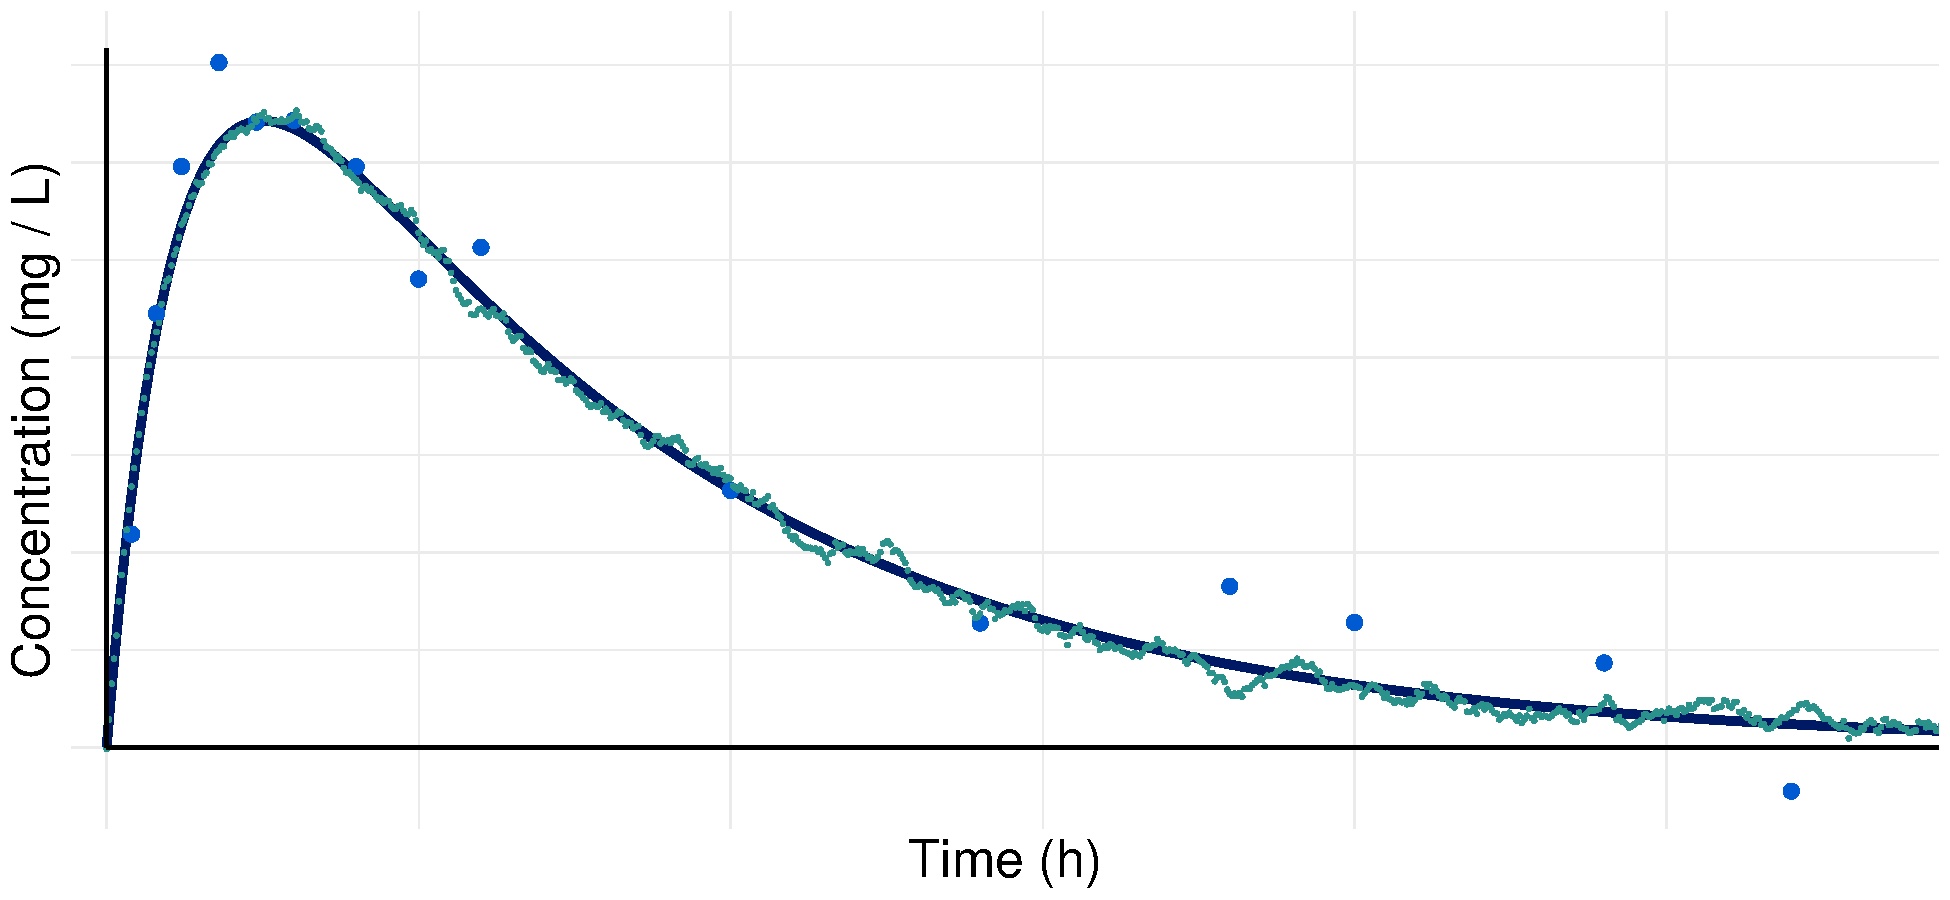
\includegraphics[width=\linewidth]{fig/img/Residual Variance Model/Measurement error.pdf}
%         \label{fig: Measurement error}
%         \caption{Concentration function, realised response profile and measurements}
%     \label{fig: Measurement error}
% \end{figure}
% If $g$ is a misspecified model, and $g +e^S_{i,j}$ is the true trajectory of the response profile, then $g$ itself is a biased representation of the true trajectory with $e^S_{i,j}$ representing systematic deviations. However, since the exact nature of the misspecification is unknown, it is hard to distinguish between bias and within-individual variation, and therefore $ e^S_{i,j}+e^R_{i,j}$ is often considered a unified source of variation. Henceforth, it is assumed that $e^S_{i,j}=0$.

% % Initially, assume that $g$ is a correctly specified model, such that $e^S_{i,j}=0$. To understand the nature of the partitioning of the residual, consider Figure \ref{fig: Measurement error}, in which the dark blue function represents $g$, whereas the blue dots represent the $n_i$ realised measurements $y_{i,j}$, and the green trajectory represents the true, but unknown, response profile of subject $i$. 

% The difference between the true response profile and $g$ is $e^R_{i,j}$; a variability mainly due to model assumptions. For instance, in a compartment model, it is assumed that the drug is being evenly distributed within the plasma, while in reality, the drug might not be perfectly mixed within the body, making the true response profile fluctuate locally around $g$ as visualised in Figure \ref{fig: Measurement error}. 

% The difference between the true response profile and the observed response measurements $y_{i,j}$ is $e^M_{i,j}$.

% Note that $g$ should be understood as an average of all possible true response profiles and measurement errors that could be observed for subject $i$, also called the inherent tendency for the response of subject $i$ over time \citep[p. 396]{Davidian2003}. This implies that NLME models are fundamentally concerned with modelling inherent tendencies of individuals, rather than the true response profiles.

% % Clearly, if it is assumed that $g$ is exactly equal to the true trajectory of the response profile, then $e_{i,j}^S+e_{i,j}^R=0$, and thus $e_{i,j}=e_{i,j}^M$.

% If the aim is to model the residuals $e^R_{i,j}$, it might make sense to allow for autocorrelation, as $e^R_{i,j}$ and $e^R_{i,j+h}$ for small $h$ would tend to be similar, while it is not the case for larger values of $h \in \Z$, as suggested by Figure \ref{fig: Measurement error}. However, within the field of PMX, the common approach is that the primary source of variation is due to $e^M_{i,j}$, and, for this reason, the term $e^R_{i,j}$ is neglected. This implies that the error that needs to be modelled is measurement error only, i.e. 
% \begin{align*}
%     e_{i,j}:=e_{i,j}^M.
% \end{align*}
% Often, it is assumed that measurement error is not autocorrelated, since it is justifiable that the error of measurement at time point $t_{i,j}$ should not depend on the error measured at time $t_{i,j+h}$ for all values of $h \in \Z$. Under this assumption,
% \begin{align}
%     \Var{e_{i} \mid \theta_i}=R_i(u_i,\theta_i,\xi) \label{eq: diag residual covariance matrix}
% \end{align}
% is a diagonal matrix depending on $u_i, \theta_i$ specified in \eqref{eq: NLME Stage 1} and \eqref{eq: NLME Stage 2}, respectively, and $\xi=(\sigma,\psi^\top)^\top$, where $\sigma$ is a constant factor, and $\psi$ is a vector of parameters. 

% Within PMX, it is assumed that measurement errors are not autocorrelated. However, it is not always plausible to assume homoscedasticity, as measurement errors often have heteroscedastic tendencies. Thus, the aim is to choose a model for the diagonal covariance matrix \eqref{eq: diag residual covariance matrix}. 

% Let $\varepsilon_i \sim (0,\sigma^2I)$ denote a random vector of dimension $n_i$. The residual error can then be represented as
% \begin{align} \label{eq: residual variance model}
%     e_{i} &=  v(t_{}, u_i, \theta_i, \psi)\varepsilon_{i},
% \end{align}
% where $v(t,u_i,\theta_i,\psi)=[v(t_{i,1},u_i,\theta_i,\psi),\dots,v(t_{i,n_i},u_i,\theta_i,\psi)]^\top \in \R^{n_i}$ denotes a function independent of $\varepsilon_i$, and $\psi$ denotes a vector of parameters. The variance of the residual error is then
% \begin{align*}
%     \Var{e_{i} \mid \theta_i} =  [v(t_{i,j}, u_i, \theta_i, \psi)]^2\sigma^2I,
% \end{align*}
% where the dependence on the random effects is emphasized through the condition on $\theta_i$. 

% The most common error models used in PMX can be seen in Table \ref{tab:error models}. 
% \begin{table}[H]
% \centering
% \begin{tabular}{>{\raggedright\arraybackslash}p{0.4\textwidth}>{\raggedright\arraybackslash}p{0.53\textwidth}}
% \toprule
% \textbf{Error model} & \textbf{Representation of $e_i$} \\
% \midrule
% Additive & $e_{i} = \varepsilon_{i}$ \\
% Proportional & $e_{i} = [g(t, u_i, \theta_i)]^2\varepsilon_{i}$ \\
% Combined additive and proportional & $e_{i} = \left( \sqrt{1-\psi + \psi g^2(t, u_i, \theta_i)}\right)\varepsilon_{i}, \quad \psi \in [0, 1]$ \\
% \bottomrule
% \end{tabular}
% \caption{Representation of the residual error, $e_i$, for the additive, proportional and combined additive and proportional error model, respectively.}
% \label{tab:error models}
% \end{table}

% The additive error model assumes constant variance, i.e. 
% \begin{align*}
%     R_i(u_i,\theta_i,\xi)=\Var{e_i \mid \theta_i}=\Var{\varepsilon_i}=\sigma^2I.
% \end{align*}
% An example of simulated data that follows the additive residual variance model can be seen in Figure \ref{fig: Residual variance model add}.

% The proportional error model allows the variance to vary over time by letting it be proportional with the non-linear function $g$,
% \begin{align*}
% R_i(u_i,\theta_i,\xi)&=\Var{e_i \mid \theta_i}=\Var{g(t,u_i,\theta_i)\varepsilon_i \mid \theta_i}=g^2(t,u_i,\theta_i,\psi)\sigma^2I\\
% &=\sigma^2 \text{diag}[g^2(t_{i,1},u_i,\theta_i), \dots, g^2(t_{i,n_i},u_i,\theta_i)].
% \end{align*}
% An example of simulated data that follows the proportional residual variance model can be seen in Figure \ref{fig: Residual variance model prop}.

% The combined additive and proportional error model exhibits properties from both models. As $\phi_k \in [0,1]$, it is possible to adjust the contribution of each model. Note that if $\psi=0$, it simplifies to an additive model, whereas if $\psi=1$, it simplifies to a proportional model. The combined additive and proportional error has covariance matrix
% \begin{align*}
% R_i(u_i,\theta_i,\xi)&=\Var{e_i \mid \theta_i}=\Var{ \left( \sqrt{1-\psi + \psi g(t, u_i, \theta_i)^2}\right)\varepsilon_{i} \mid \theta_i} \\
%     &= \left[1-\psi + \psi g(t, u_i, \theta_i)^2\right] \sigma^2I\\
%     &=\sigma^2 \text{diag}\left[(1-\psi + \psi g(t_{i,1}, u_i, \theta_i)^2),\dots,(1-\psi + \psi g(t_{i,n_i}, u_i, \theta_i)^2)\right].
% \end{align*}
% An example of simulated data that follows the combined additive and proportional residual variance model can be seen in Figure \ref{fig: Residual variance model add prop}.

% \begin{figure}[H]
%     \centering
%     \begin{minipage}{0.45\textwidth}
%         \centering
%         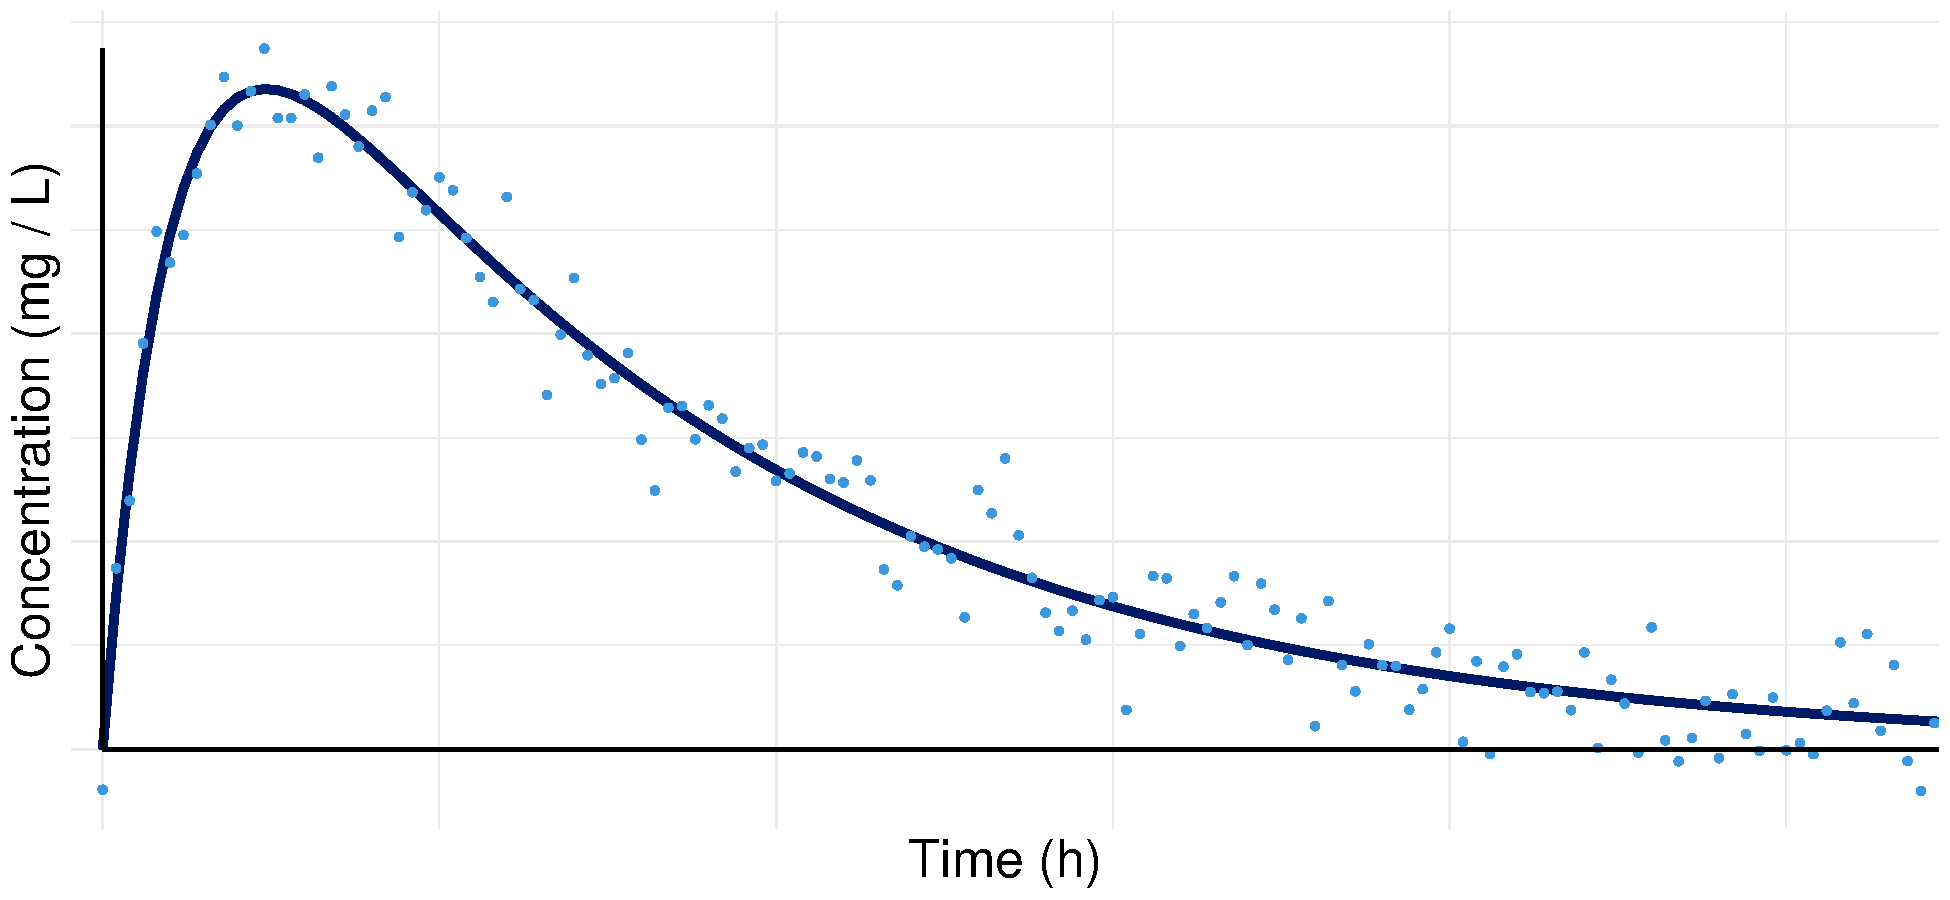
\includegraphics[width=\linewidth]{fig/img/Residual Variance Model/Concentration W. Oral Add.pdf}
%         \caption{Additive error}
%         \label{fig: Residual variance model add}
%     \end{minipage}%
%     \hfill
%     \begin{minipage}{0.45\textwidth}
%         \centering
%         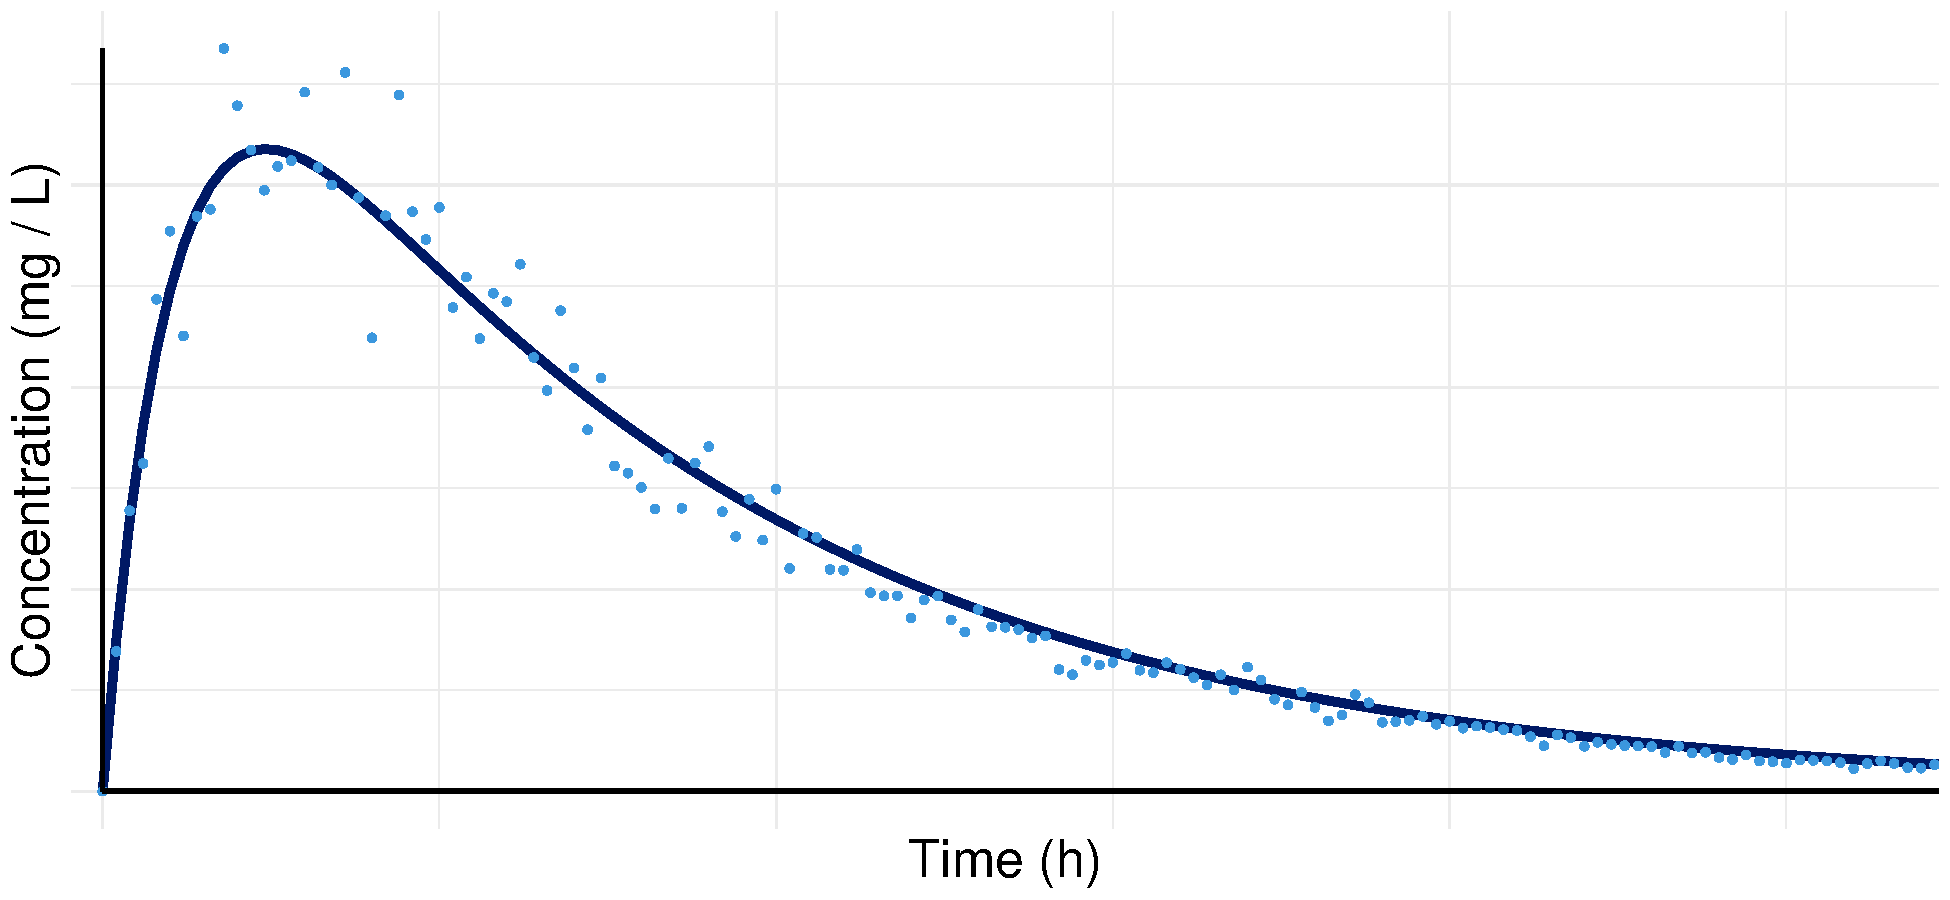
\includegraphics[width=\linewidth]{fig/img/Residual Variance Model/Concentration W. Oral Prop.pdf}
%         \caption{Proportional error}
%         \label{fig: Residual variance model prop}
%     \end{minipage}
%     \vfill

%     \begin{minipage}{0.45\textwidth}
%         \centering
%         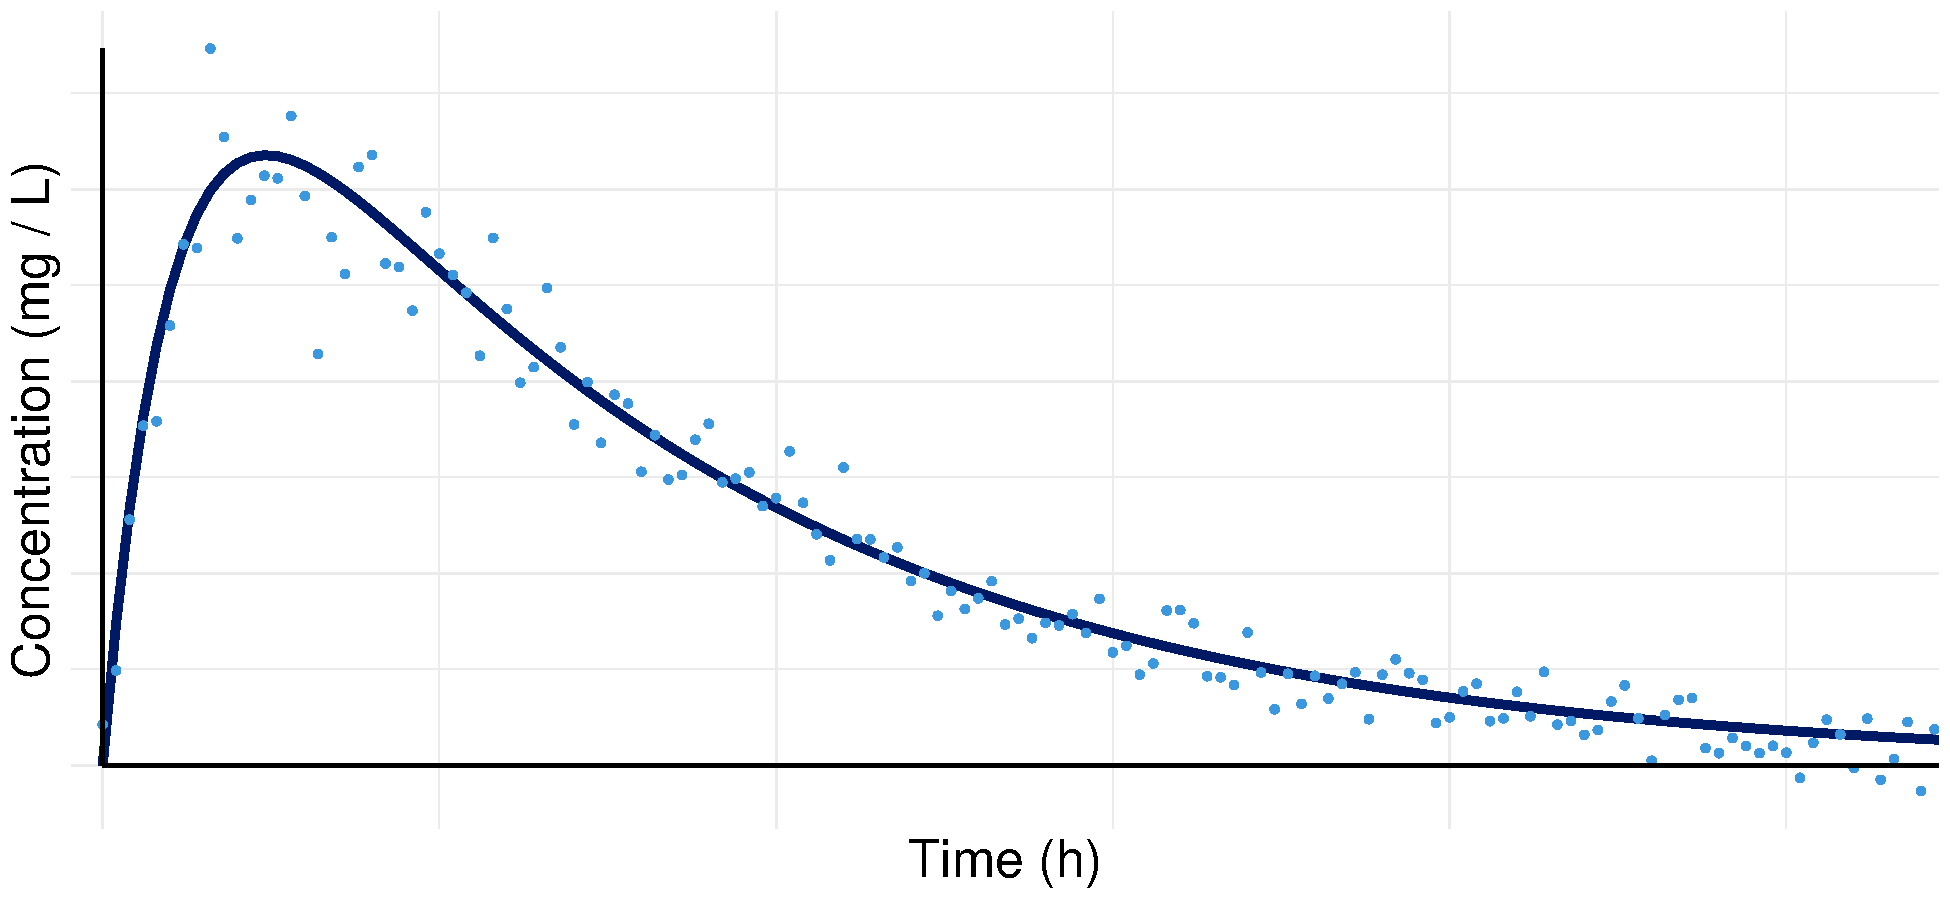
\includegraphics[width=\linewidth]{fig/img/Residual Variance Model/Concentration W. Oral Add Prop.pdf}
%         \caption{Combined additive and proportional error}
%         \label{fig: Residual variance model add prop}
%     \end{minipage}
%     \caption{Simulated concentrations from a single dose one-compartment model with EV administration, each with different error models.}
%     \label{fig: Residual variance model}
% \end{figure}
% To determine which residual variance model is most suitable, likelihood ratio tests and goodness of fit plots are used. 

\section{Residual variability}

While $\Omega \in \R^{r \times r}$ contains the BSV, the remaining unexplained variability is contained in $R_i(u_i,\theta_i,\xi)$, for $i=1,\dots,N$, and is considered the collection of within-subject variability, measurement error, and model misspecification. If $g(t_{ij},u_i,\theta_i)$ is correctly specified and $f_{ij}$ denotes the true, but unobserved, response at time $t_{ij}$, then the residual error can be considered the sum $e_{i,j}=e^M_{i,j}+e^R_{i,j}$, where $e^M_{i,j}=y_{ij}-f_{ij}$ is measurement error, and $e^R_{i,j}=f_{ij}-g(t_{ij},u_i,\theta_i)$ is within-subject variation.

In PMX, a common approximation is that residual error primarily arises from measurement error \citep{Karlsson1995}. It is standard that measurement errors at different time points, $t_{i,j}$ and $t_{i,j+h}$, are assumed independent for all $h \in \Z$, thus $R_i(u_i,\theta_i,\xi)$ is modelled as diagonal \citep[p. 398]{Davidian2003}.

In practice, measurement errors tend to vary as a function of $g(t_{ij},u_i,\theta_i)$, causing heteroscedasticity \citep[p. 398]{Davidian2003}. To account for this, it is necessary to specify an appropriate structure for $R_i(u_i,\theta_i,\xi)$. The most common error models utilised in PMX are the additive (add.), proportional (prop.), and combined add. and prop., which are detailed in Table \ref{tab:error models}. 

\begin{table}[h]
\centering
\begin{tabular}{>{\raggedright\arraybackslash}p{0.16\textwidth} >{\raggedright\arraybackslash}p{0.26\textwidth} >{\raggedright\arraybackslash}p{0.49\textwidth}}
\toprule
\textbf{Error model} & \textbf{Representation of $e_i$} & \textbf{Structure of $R_i(u_i,\theta_i,\xi)$} \\
\midrule
Add. & $\varepsilon_{i,add}$ & $\sigma^2_{add}I$ \\
Prop. & $g(t, u_i, \theta_i)\varepsilon_{i,prop}$ & $\sigma_{prop}^2 \text{diag}[g^2(t_{i,1},u_i,\theta_i), \dots, g^2(t_{i,n_i},u_i,\theta_i)]$ \\
Add./prop. & $g(t, u_i, \theta_i)\varepsilon_{i,prop}+\varepsilon_{i,add}$ & $\sigma_{prop}^2 \text{diag}[g^2(t_{i,1},u_i,\theta_i), \dots, g^2(t_{i,n_i},u_i,\theta_i)] + \sigma^2_{add}I$ \\
\bottomrule
\end{tabular}
\caption{Representation of the residual error, $e_i$, through $\varepsilon_{i,add} \sim (0,\sigma^2_{add}I)$ and $\varepsilon_{i,prop} \sim (0,\sigma^2_{prop}I)$, for the additive, proportional and combined additive and proportional error model, respectively \citep[p. 236]{bonate}.}
\label{tab:error models}
\end{table}

The additive error assumes homoscedasticity, suitable when the residual error is independent of the magnitude of $g(t_{ij},u_i,\theta_i)$. The proportional error accounts for heteroscedasticity, where the residual error increases with $g(t_{ij},u_i,\theta_i)$. When the residual error structure is uncertain, a combined additive and proportional model can be used. 

An additive error model can inappropriately yield negative concentrations, see Figure \ref{fig: Residual variance model add}, which is avoided with the proportional error model, see Figure \ref{fig: Residual variance model prop}.

% The additive error assumes constant variance, and is suitable when the residual error is independent of the magnitude of the observations. An example of simulated data that follows the additive residual variance model is depicted in Figure \ref{fig: Residual variance model add}.

% The proportional error assumes heteroscedasticity, and is suitable when the variance increases with the magnitude of the prediction. 

% If the error structure is uncertain, the combined additive and proportional error can be used instead. An example of simulated data that follows the combined additive and proportional residual variance model can be seen in Figure \ref{fig: Residual variance model add prop}.


% The structure of $R_i(u_i,\theta_i,\xi)$ for each residual variance model is shown in \ref{eq: add. error}, \ref{eq: prop error}, and \ref{eq: add prop error}, respectively. 

% The additive error model assumes constant variance, i.e. 
% \begin{align}
%     R_i(u_i,\theta_i,\xi)=\Var{e_i \mid \theta_i}=\Var{\varepsilon_{i,add}}=\sigma^2_{add}I. \label{eq: add. error}
% \end{align}
% An example of simulated data that follows the additive residual variance model can be seen in Figure \ref{fig: Residual variance model add}.

% The proportional error model allows the variance to vary over time by letting it be proportional with the non-linear function $g$,
% \begin{align}
% R_i(u_i,\theta_i,\xi)&=\Var{e_i \mid \theta_i}=\Var{g(t,u_i,\theta_i)\varepsilon_{i,prop} \mid \theta_i}=g^2(t,u_i,\theta_i,\psi)\sigma_{prop}^2I\nonumber \\
% &=\sigma_{prop}^2 \text{diag}[g^2(t_{i,1},u_i,\theta_i), \dots, g^2(t_{i,n_i},u_i,\theta_i)]. \label{eq: prop error}
% \end{align}
% An example of simulated data that follows the proportional residual variance model can be seen in Figure \ref{fig: Residual variance model prop}.

% The combined additive and proportional error model exhibits properties from both models. As $\phi_k \in [0,1]$, it is possible to adjust the contribution of each model. Note that if $\psi=0$, it simplifies to an additive model, whereas if $\psi=1$, it simplifies to a proportional model. The combined additive and proportional error has covariance matrix
% \begin{align}
% R_i(u_i,\theta_i,\xi)&=\Var{e_i \mid \theta_i}=\Var{ \left( \sqrt{1-\psi + \psi g(t, u_i, \theta_i)^2}\right)\varepsilon_{i} \mid \theta_i} \\
%     &= \left[1-\psi + \psi g(t, u_i, \theta_i)^2\right] \sigma^2I \nonumber \\
%     &=\sigma^2 \text{diag}\left[(1-\psi + \psi g(t_{i,1}, u_i, \theta_i)^2),\dots,(1-\psi + \psi g(t_{i,n_i}, u_i, \theta_i)^2)\right]. \label{eq: add prop error}
% \end{align}
% An example of simulated data that follows the combined additive and proportional residual variance model can be seen in Figure \ref{fig: Residual variance model add prop}.

\begin{figure}[h]
    \centering
    \begin{minipage}{0.45\textwidth}
        \centering
        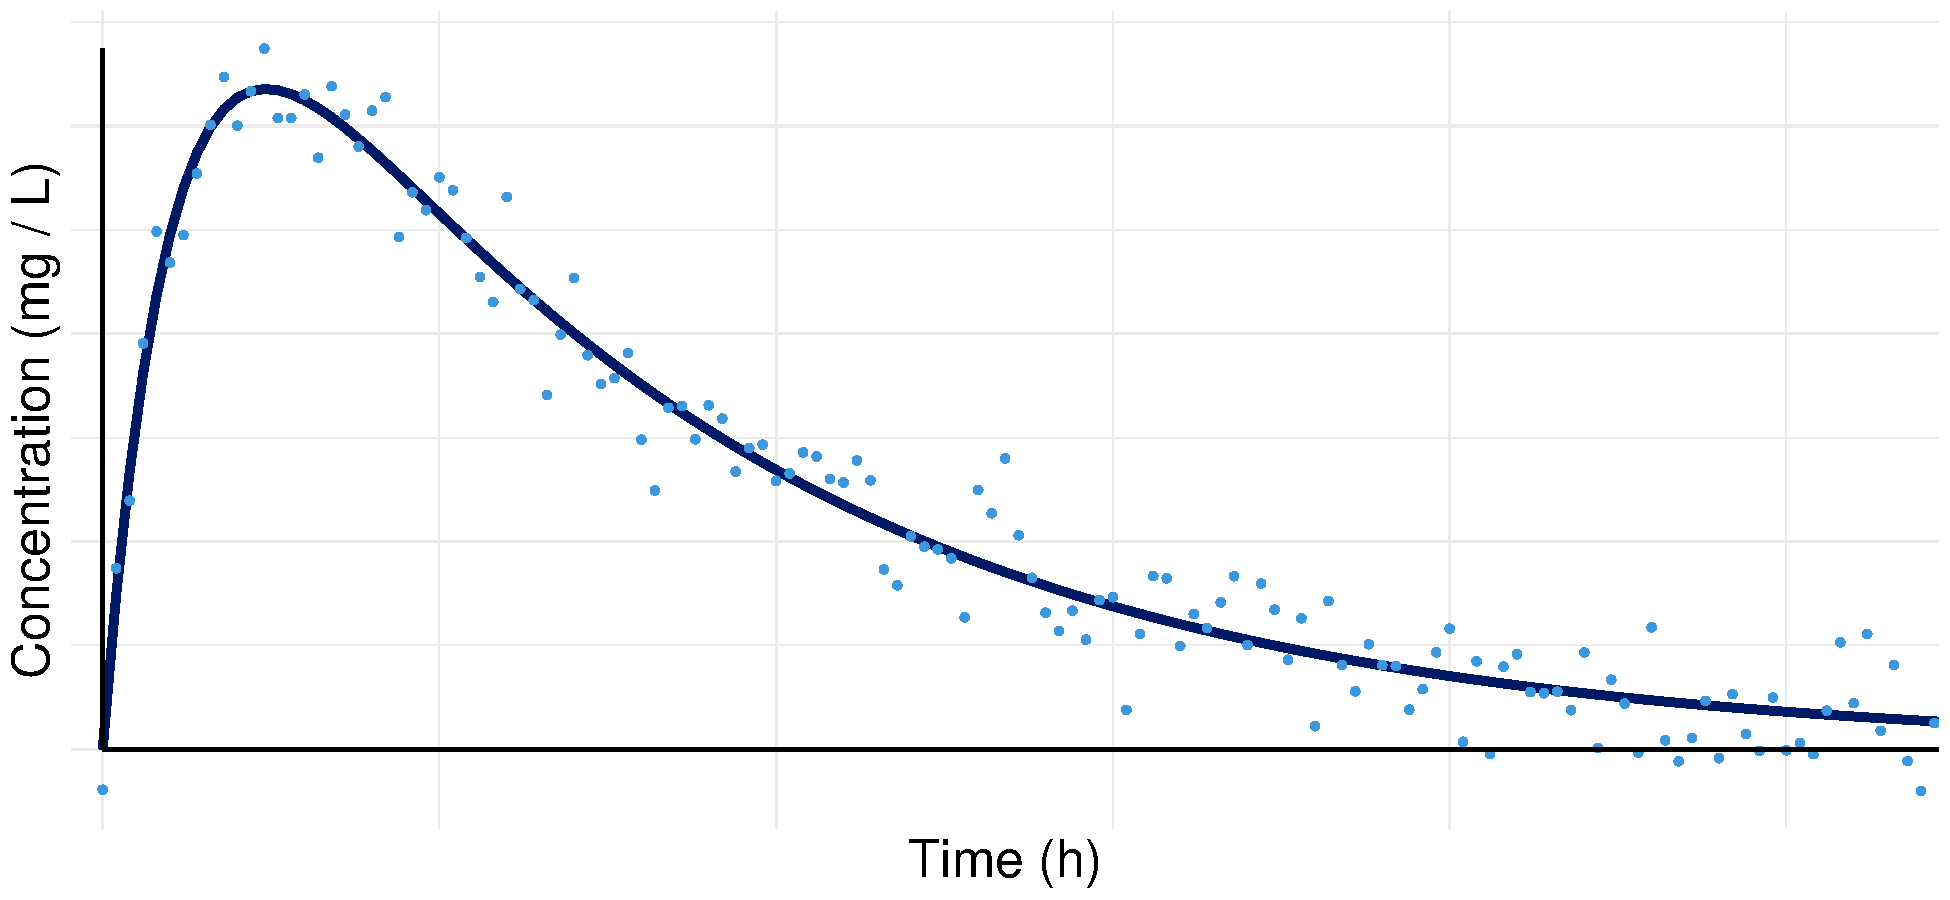
\includegraphics[width=\linewidth]{fig/img/Residual Variance Model/Concentration W. Oral Add.pdf}
        \caption{Additive error}
        \label{fig: Residual variance model add}
    \end{minipage}%
    \hfill
    \begin{minipage}{0.45\textwidth}
        \centering
        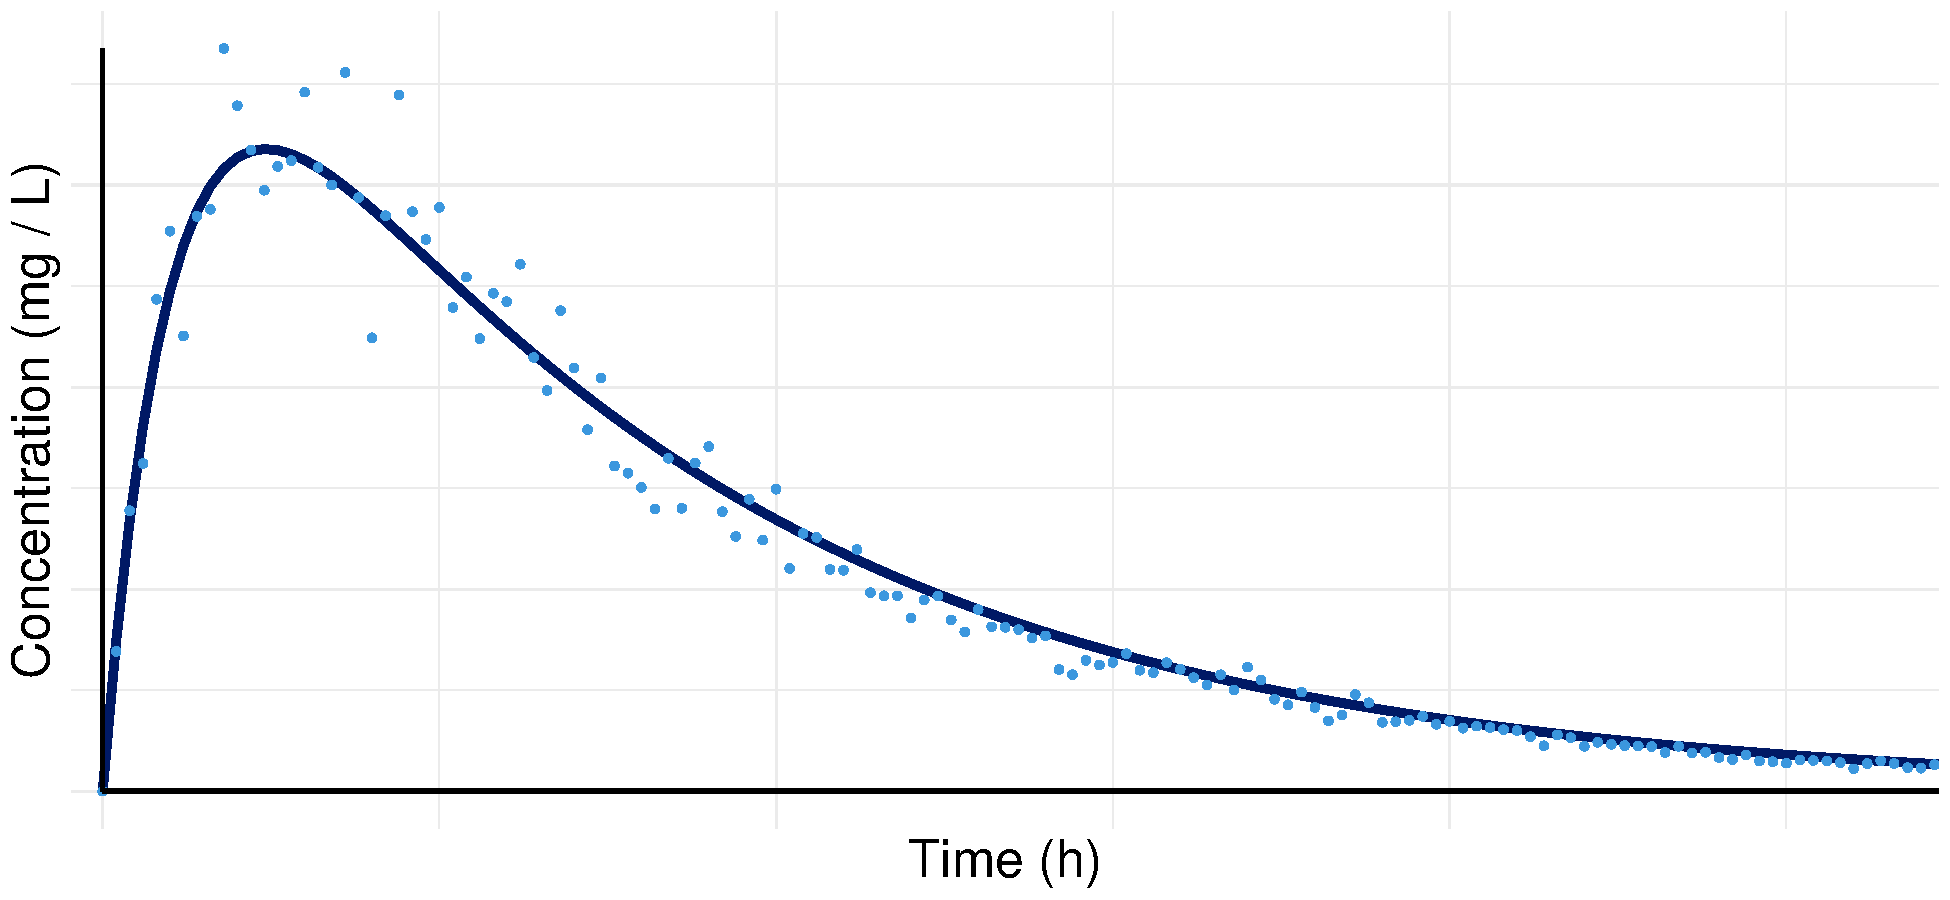
\includegraphics[width=\linewidth]{fig/img/Residual Variance Model/Concentration W. Oral Prop.pdf}
        \caption{Proportional error}
        \label{fig: Residual variance model prop}
    \end{minipage}
    \caption{Simulated concentrations from a one-compartment model with oral administration, each with different error models.}
    \label{fig: Residual variance model}
\end{figure}
% To determine which error model is most suitable, likelihood ratio tests and goodness of fit plots are used. 

\section{Estimation methods} \label{sec: Estimation methods}
% Let $g_i(\theta_i):=[g(t_{i,1}, u_i, \theta_i), g(t_{i,2}, u_i, \theta_i), \dots, g(t_{i,n_i}, u_i, \theta_i)]^\top \in \R^{n_i}$ denote the vector of mean responses for each time point measured for the $i$'th subject, and let $e_i = (e_{i,1}, \dots, e_{i,n_i})^\top \in \R^{n_i}$ denote the random errors for subject $i$.  The model specified by \eqref{eq: NLME Stage 1} and \eqref{eq: NLME Stage 2} can then be written as 
% \begin{align}
%     y_i &= g_i(\theta_i)+e_i, \quad e_i\mid \theta_i \sim (0,R_i(u_i,\theta_i,\xi)), \label{eq: stage 1 for subject i}\\
%     \theta_i &= d(a_i,\beta,\eta_i), \quad \eta_i \sim (0,\Omega)\label{eq: stage 2 for subject i},
% \end{align}
% for $i = 1,\dots,N$. The set of parameters to be estimated are $\beta \in \R^k$, $\xi=(\sigma,\psi^\top)^\top$ and $\Omega$. Here, $\beta$ and $\Omega$ are considered population parameters. To estimate these parameters, the aim is to derive the likelihood function for $\beta$, $\xi$ and $\Omega$. 

% \subsection{The Likelihood Function}
Fundamental to NLMM is the fact that \eqref{eq: NLME Stage 1} requires an assumption about the distribution of $\eta_i$, while \eqref{eq: NLME Stage 2} requires an assumption about the distribution of $y_i \mid \eta_i$, as $y_i$ depends on $\eta_i$ through $\theta_i$. Thus, the joint density of $(y_i, \eta_i)$ is given by
\begin{align*}
    p_{y,\eta}(y_i,\eta_i\mid x_i,\beta,\xi,\Omega)=p_{y\mid \eta}(y_i\mid x_i,\eta_i,\beta,\xi)p_\eta(\eta_i\mid \Omega),
\end{align*}
where $p_{y\mid  \eta}$ is the conditional density of $y_i \mid \eta_i$, and $p_\eta$ is the density of $\eta_i$. Remind that $x_i =(u_i,a_i)$ is the collection of covariates for subject $i$. The random effects serve as latent variables, implying that $\eta_i$ is unobservable. Consequently, a marginalisation w.r.t. $\eta_i$ yields the marginal distribution of $y_i$,
\begin{align}
    p_y(y_i\mid x_i,\beta,\xi)=\int_{\R^r} p_{y\mid \eta}(y_i\mid x_i,\beta,\eta_i,\xi)p_\eta(\eta_i\mid  \Omega)d\eta_i. \label{eq: marginal distribution of y_i}
\end{align}

The likelihood function for $\beta$, $\xi$, $\Omega$ can be expressed as the joint density of the observed data $y_1,y_2,\dots,y_N$ given $x_i$, which, by independence across $i$, is given by the product of the marginal densities \eqref{eq: marginal distribution of y_i},
\begin{align}
    L(\beta,\xi,\Omega\mid  y_1,y_2,\dots,y_N)&=\prod_{i=1}^N  p_y(y_i\mid x_i,\beta,\xi)  \nonumber \\&=\prod_{i=1}^N\int_{\R^r} p_{y\mid \eta}(y_i\mid x_i,\beta,\eta_i,\xi)p_\eta(\eta_i\mid  \Omega)d\eta_i.\label{eq: likelihood for parameters}
\end{align}
The $N$ $r$-dimensional integrations that appear in \eqref{eq: likelihood for parameters} do not have a closed form expression -- neither when normality is assumed. This is due to the fact that the estimation of $\xi$ depends on the estimation of $\Omega$, i.e. $e_i$ is dependent on $\eta_i$, further complicated by the non-linearity of $g(\cdot)$. Instead, the integration must be done by numeric approximation.

\section{Estimation methods used in nlmixr}
Vi tager udgangspunkt i FOCE-i algoritmen, FOCE og FO er simplere specialtilfælde. Denne metode bruger en approksimation af likelihood-funktionen - her findes flere metoder til dette. Det approksimerede likelihood skal maksimeres (outer optimisation problem), men det er baseret på et fast estimat for de random effects, som også skal estimeres (inner problem). 

The default inner optimisation algorithm used in nlmixr is a Quasi-Newton Broyden–Fletcher–Goldfarb–Shanno (BFGS) algorithm without constraints which is an iterative method for solving unconstrained nonlinear optimization problems. The package used is 'n1qn1' which allows prespecification of Hessian. This package is an R port of the optimisation procedure in scilab.


This inner optimisation problem needs specification og the objective function (call\_eval), the gradient function (call\_grad) and the initial starting point for line search (vars). Så hvad er objective og gradient function?

kan ex. være en Laplace transformation med second order Taylorudvikling af g(eta) omkring eta (EBE). EBE skal også estimeres 


\subsection{The Likelihood under Normality}
By the assumption of normality, i.e. $e_i\mid \theta_i \sim N(0,R_i)$ and $\eta_i \sim N(0,\Omega)$, the densities $p_{y\mid \eta}$ and $p_{\eta}$ are given by
\begin{align*}
    p_{y\mid \eta}(y_i\mid x_i,\beta,\eta_i,\xi) &= \frac{1}{(2\pi)^{n_i/2}\mid R_i\mid ^{1/2}}\exp{\left(-\frac{1}{2}\left[y_i-g_i(\theta_i)\right]^\top R_i^{-1}\left[y_i-g_i(\theta_i)\right]\right)},\\
    p_\eta(\eta_i\mid \Omega)&=\frac{1}{(2\pi)^{r/2}\mid \Omega\mid ^{1/2}}\exp{\left(-\frac{1}{2}\eta_i^\top \Omega^{-1}\eta_i\right)}.
\end{align*}

The marginal density of $y_i$ is then
\begin{align}
    p_y(y_i\mid x_i,\beta,\xi)=\int_{\R^r}(2\pi)^{-(n_i-r)/2}|R_i|^{-1/2}|\Omega|^{-1/2}\exp{\left(-\frac{1}{2}\Psi(\eta_i)\right)d\eta_i}, \label{eq: marginal distribution of y_i under normality}
\end{align}
where $\Psi(\eta_i)=\left(y_i-g_i(\theta_i)\right)^\top|R_i|^{-1}\left(y_i-g_i(\theta_i)\right)+\eta_i^\top|\Omega|^{-1}\eta_i$. 

Insert \eqref{eq: marginal distribution of y_i under normality} as $p_y$ in \eqref{eq: likelihood for parameters} to get the likelihood function for $\beta$, $\xi$, $\Omega$ under the assumption of normality.

\subsection{FOCE-i}
Kilder brugt: \cite{Almquist2015}, \cite{Bae2016}, \cite{Savic2009}, \cite{Wang2007}, \cite{Davidian1995}.

Focei estimation is the general method including the simpler versions foce and fo. 

Given a complex integral, $ \int_\Omega f(x) \ dx$, with $f$ twice differentiable, and $f(x)>0 \ \forall x \in \Omega$, $f(x)$ can be expressed as $\exp g(x)$ with $g(x)=\log f(x)$. If $\frac{d^2 g(x)}{d x^2}\big\rvert_{x=x_0}<0$, then
\begin{align*}
    \int_\Omega f(x) \ dx &\approx \int_\Omega \exp g(x_0) +(x-x_0) \cdot\frac{d g(x)}{d x}\Big\rvert_{x=x_0} +\frac{(x-x_0)^2}{2!} \cdot \frac{d^2 g(x)}{d x^2}\Big\rvert_{x=x_0}\ dx
    % &=f(x_0) \cdot \sqrt{\frac{(2\pi)^r}{\left|-\frac{d g(x)}{d^2 x}\Big\rvert_{x=x_0}\right|}}
\end{align*}
is the Laplacian approximation of the true integration, obtained using a second-order Taylor expansion of $g(x)$ around $x_0$. 

Laplacian approximation can be used to approximate \eqref{eq: likelihood for parameters} by letting $f(\eta_i)=p_{y\mid  \eta}\cdot p_\eta$ denote the joint density under the assumption of normality. Then
\begin{align*}
    g(\eta_i)=\log\left[\frac{1}{(2\pi)^{n_i/2}|R_i|^{1/2}}\right]-\frac{1}{2}\left[e_i^\top R_i e_i\right] + \log \left[\frac{1}{(2\pi)^{r/2}|\Omega|^{1/2}}\right] -\frac{1}{2}\left[\eta_i^\top \Omega \eta_i\right].
\end{align*}
The focei estimation method uses the Laplacian approximation with a Taylor expansion of $g(\eta_i)$ around $\eta_i^\ast = \arg \max g(\eta_i)$, i.e. the posterior mode of $g(\eta_i)$, ensuring the term of the Taylor expansion including the first derivative equals zero. Let $\Delta_i(\eta_i)=\frac{d g(\eta_i)}{d^2 \eta_i}$ denote the Hessian matrix.
% If the Taylor expansion is done around $\eta_i^\ast$, where $g'(\eta_i^\ast)=0$, it simplifies to
% \begin{align*}
%     \int_{\R^r} f(\eta_i) d\eta_i=\int_{\R^r} \exp(g(\eta_i)) d\eta_i \approx f(\eta_i^\ast) \cdot \sqrt{\frac{(2\pi)^r}{\left|-\frac{d g(\eta_i)}{d^2 \eta_i}\Big\rvert_{\eta_i=\eta_i^\ast}\right|}}.
% \end{align*}
The approximation of \eqref{eq: likelihood for parameters} is then
\begin{align}
    L(\beta,\xi,\Omega\mid  y_1,y_2,\dots,y_N)&\approx \prod_{i=1}^N\int_{\R^r} \exp g(\eta_i^\ast) +\frac{(\eta_i-\eta_i^\ast)^2}{2!} \Delta_i(\eta_i^\ast)\ d\eta_i \nonumber \\
    &= f(\eta_i^\ast) \cdot \sqrt{\frac{(2\pi)^r}{\left|-\Delta_i(\eta_i^\ast)\right|}}.\label{eq: approx laplace likelihood}
\end{align}
% \begin{align}
%     L(\beta,\xi,\Omega\mid  y_1,y_2,\dots,y_N)&\approx \prod_{i=1}^N f(\eta_i^\ast) \cdot \sqrt{\frac{(2\pi)^r}{\left|-\Delta_i(\eta_i^\ast)\right|}}. 
% \end{align}
The last equality is obtained using the moment generating function of a normal random variable, with derivations provided in \cite{Wang2007} (pp. 588-589). 

The focei objective function is obtained by multiplying \eqref{eq: approx laplace likelihood} by $-2$, taking the logarithm, and using an estimate of the Hessian matrix, $\hat\Delta_i$, i.e.
\begin{align*}
    O_{focei}&=\sum_{i=1}^N -2\log p_{y|\eta}(\eta_i^\ast)-2\log p_\eta(\eta_i^\ast)-\log \frac{(2\pi)^r}{\left|-\hat\Delta_i(\eta_i^\ast)\right|}\\
    &= \sum_{i=1}^N-2\log p_{y|\eta}(\eta_i^\ast) +\log|\Omega|+{\eta_i^\ast}^\top \Omega^{-1} \eta_i^\ast +\log \left|-\hat\Delta_i(\eta_i^\ast)\right|,
\end{align*}
where $\hat\Delta_i$ is approximated 
by a function of the gradient vector, ignoring the second order derivatives that are costly to compute. The exact form of the elements of $\hat\Delta_i$ are derived in \cite{Almquist2015} (pp. 193-194).


In the outer optimisation problem, $O_{focei}$ is minimised for fixed values of $\eta_i^\ast$ to update estimates of $\beta,\xi,\Omega$. The inner optimisation, $\eta_i^\ast = \arg \max g(\eta_i)$, is done in each step for fixed values of $\beta,\xi,\Omega$ to update estimates of $\eta_i^\ast$ to be inserted in $O_{focei}$. 

The final estimate of $\hat{\eta_i}$ have an empirical Bayes interpretation (Gilt, 1995), used to determine shrinkage of the subject specific parameters. 

% Shrinkage is defined as
% \begin{align*}
%     \eta_{shrink} = 1 - \frac{SD(\hat{\eta})}{\omega}
% \end{align*}

\subsection{First-Order Estimation}
FO: No (small) IIV, assumes additive error model. No inner optimisation problem. FOCE: Additive error model. FOCE-i: Proportional (or combined) error model. Generally two methods: Laplacian approximation and linearisation. These two methods yield equivalent objective functions for FO and FOCE, however not for FOCE-i. NONMEM uses the Laplacian approximation. (WANG). What does nlmixr use? FOCE-i, innerOpt = c("n1qn1", "BFGS"), outerOpt = c("nlminb", "bobyqa", "lbfgsb3c", "L-BFGS-B", "mma", "lbfgsbLG", "slsqp",
"Rvmmin").
The first-order (FO) method models a linear approximation of \eqref{eq: likelihood for parameters} using a Taylor expansion around $\eta_i=0$. The method uses a Cholesky decomposition of $R_i$, 

Since $R_i(u_i,\theta_i,\xi)$ is diagonal, its Cholesky decomposition is simply $R_i=R_i^{1/2}R_i^{1/2}$. Let $\epsilon_i \sim (0,I_{n_i})$ and write the residual error as $e_i=R_i^{1/2}\epsilon_i$. This rewriting is justified since $\Ex{e_i \mid \theta}=\Ex{R_i^{1/2}\epsilon_i}=0$ and $\Var{e_i \mid \theta_i}=\Var{R_i^{1/2}\epsilon_i \mid \theta_i }=R_i^{1/2}\Var{\epsilon_i}R_i^{1/2}=R_i$. The model \eqref{eq: NLME Stage 1} can then be written as 
\begin{align*}
    y_i &= g_i(\theta_i) + R_i^{1/2}(u_i,\theta_i,\xi)\epsilon_i \\
    &= g_i(d(a_i,\beta,\eta_i)) + R_i^{1/2}(u_i,d(a_i,\beta,\eta_i),\xi)\epsilon_i, \quad \epsilon_i \sim N(0,I_{n_i}),
\end{align*}
where the dependence on the $\eta_i$'s are written explicitly.

The idea is then to use a Taylor expansion around $\eta_i=0$. This yields the first order approximation of $y_i$,
\begin{align}
    y_i \approx g_i(d(a_i,\beta,0)) + R_i^{1/2}(u_i,d(a_i,\beta,0),\xi)\epsilon_i + (derivA + derivB)\eta_i. \label{eq: FO approx}
\end{align}
The last term is omitted, as misspecification of second order moments is not as crucial as for first order moments (kilde). Denote derivA $:= Z_i(\beta,0)$ and $e_i^{\ast}:= R_i^{1/2}(u_i,d(a_i,\beta,0),\xi)\epsilon_i$ to get the representation 
\begin{align*}
       y_i \approx g_i(d(a_i,\beta,0)) + Z_i(\beta,0)\eta_i + e_i^{\ast}. 
\end{align*}
The approximated marginal first and second moment of $y_i$ is then
\begin{align*}
    \Ex{y_i} &\approx g_i(d(a_i,\beta,0)),\\
    \Var{y_i} &\approx \Var{Z_i(\beta,0)\eta_i} + \Var{e_i^{\ast}}\\
    &= Z_i(\beta,0)\Var{\eta_i}Z_i^{\top}(\beta,0) + R_i^{1/2}(u_i,d(a_i,\beta,0),\xi)\Var{\epsilon_i}R_i^{1/2}(u_i,d(a_i,\beta,0),\xi)\\
    &=  Z_i(\beta,0)\Omega Z_i^{\top}(\beta,0) + R_i^{1/2}(u_i,d(a_i,\beta,0),\xi)\\
    &=:V_i(\beta,0,\xi,\Omega).
\end{align*}
Under the assumption of normality, i.e. $e_i \sim N(0,V_i(\beta,0,\xi,\Omega))$ and $\eta_i \sim N(0,\Omega)$, the marginal density of $y_i$ is
\begin{align*}
        p_{y}(y_i\mid x_i,\beta,\xi,D) &= \frac{1}{(2\pi)^{n_i/2}\mid V_i(\cdot)\mid ^{1/2}}\exp{\left(-\frac{1}{2}Q(\cdot)\right)},
\end{align*}
where $Q(\cdot)=\left[y_i-g_i(d(a_i,\beta,0))-Z_i(\beta,0)\eta_i\right]^\top V_i^{-1}(\cdot)\left[y_i-g_i(d(a_i,\beta,0))-Z_i(\beta,0)\eta_i\right]$. The likelihood is then given by
\begin{align*}
    L(\beta,\xi,\Omega \mid y_1,\dots,y_N)=\prod_{i=1}^N p_{y}(y_i\mid x_i,\beta,\xi,D),
\end{align*}
and thus the log likelihood is
\begin{align*}
    l(\beta,\xi,\Omega \mid y_1,\dots,y_N)=\sum_{i=1}^N p_{y}(y_i\mid x_i,\beta,\xi,D) \propto \sum_{i=1}^N-\frac{1}{2}\log|V_i(\cdot)|-\frac{1}{2}Q.
\end{align*}
Multiply this with $-2$ to get the objective function to be minimised,
\begin{align*}
L_{FO}=\sum_{i=1}^N\log|V_i(\cdot)|+Q(\cdot),
\end{align*}
This is therefore equal to twice the negative normal log likelihood under assumption \eqref{eq: FO approx}.

Minimisation of the objective function is done using different optimisation methods.

\section{yap}
\begin{itemize} 
    \item Taylor approx. (linearisation)
    \item Derive moments of approximated yi
    \item Assume normality => derive marginal distribution of y to derive the log likelihood
    \item Derive the objective function
    \item Optimisation - explain what there is and possible methods
\end{itemize}
Approksimation af likelihood - dernæst skal den optimeres vha. metode fra nlmixr. Ved FOCE og FOCE-i findes inner/outer optimisation problem, da vi både skal estimere eta'er, der bruges som conditional estimates for at optimere population parameters.

Fiddler skrev i august 24', at NONMEM bruger "proprietary closed source optimization algorithm" til at optimere likelihood. link \url{https://github.com/nlmixr2/nlmixr2/discussions/257}, så...? Generelt har nlmixr flere optimeringsmuligheder.



The assumptions are
\begin{align*}
    \Ex{e_i \mid  \theta_i}&=0,\\
    \Var{e_i\mid \theta_i}&=R_i(u_i,\theta_i,\xi), \quad \xi=(\sigma,\psi^\top)^\top.
\end{align*}

The integral in \eqref{eq: marginal distribution of y_i} cannot be analytically expressed. Instead, the integration must be done by numeric approximation. The integral is intractable since the estimate of $\xi$ depends on the estimate of $\Omega$, i.e. estimation of $e_i$ depends on the estimation of $\eta_i$. Moreover, the non-linearity of $g(\cdot)$ further complicates the evaluation of the integral.


=> Påbegynd estimationsmetoder


Options in nlmixr
\begin{itemize}
    \item FO: first order approximation - algorithm which transforms the NLME model into a linear ME model through a first-order Taylor approximation around the vector $\eta =0$; the model is then estimated based on the linear approximaiton to the non-linear model.
    \item FOCE: first order conditional estimation (see Wang 2009) - first order taylor approximation around the posterior mode of $\eta$, thus it depends on a conditional estimate of $\eta$
    \item FOCE-I: first order conditional estimation with interaction - same as foce, but it also accounts for interaction between $\eta$ and $e$ (e.g. proportional random error model). This method not useful when residual variance is large or $n_i$'s are small, neither for homoscedastic error models.

    \item FO-I: first order with interaction

    \item SAEM: stochastic approximation expectation-maximization
\end{itemize}
Andre metoder er til population-only data og ikke mixed effects modeller.


NONMEM 
\begin{itemize}
    \item First Order Conditional Estimation (FOCE)
    \item Laplace Conditional Estimation
    \item Iterative Two Stage (ITS) 
    \item Importance Sampling Expectation-Maximization (IMP)
    \item Stochastic Approximation Expectation-Maximization (SAEM)
    \item Markov-Chain Monte Carlo Bayesian Analysis (BAYES, NUTS) 
\end{itemize}

\subsection{First-order conditional estimation (FOCE)}
\subsection{First-order conditional estimation with interaction (FOCEi)}
This FOCEi likelihood has been compared to NONMEM’s objective function and gives the same values (based on the data in Wang 2007 (2007))
\subsection{Stochastic Approximation Expectation-Maximization}
The Expectation-Maximaization (EM) algorithm will be explained. The algorithm is useful for maximum likelihood estimation for parameters when latent variables are present. When estimating PK models with NLMEM the laten variables are the subject specific parameters. 

The log likelihood of the concentration is
\begin{align*}
    \ell (\beta) = \log p(y;\beta) = \log \int p(y,\theta;\beta) dz
\end{align*}
where $\beta = (\beta_1, \dots, \beta_k)^{\top}$ is the parameters we wish to maximize, while $p(y,\theta)$ is the joint distribution of the concentration and the subject-specific parameters. As $\theta$ is unobserved the likelihood marginalize over $\theta$. Due to the marginalization, the likelihood can be difficult to obtain analytically. Instead the EM-algorithm can be used. 

To understand how the EM-algorithm works, a Q-function will be derived from the log-likelihood
\begin{align*}
    \ell (\beta; y) &= \log \int p(y,\theta | \beta)\\
    &= \log \int \frac{p(y,\theta|\beta)}{p(\theta|y,\hat{\beta}^{(t)})}p(\theta|y,\hat{\beta}^{(t)}) d\theta\\
    &=\log \mathbb{E}_{\theta| y, \hat{\beta}^{(t)}}\left[{\frac{p(y,\theta|\beta)}{p(\theta|y,\hat{\beta}^{(t)})}}\right]\\
    &\geq \mathbb{E}_{y,\theta| y, \hat{\beta}^{(t)}}\left[{\log\frac{p(\theta|\beta)}{p(\theta|y,\hat{\beta}^{(t)})}}\right] \\
    &=\mathbb{E}_{\theta| y, \hat{\beta}^{(t)}}\left[\log p(y,\theta| \beta) \right] - \mathbb{E}_{\theta| y, \hat{\beta}^{(t)}}\left[\log p(\theta| y, \hat{\beta}^{(t)}) \right]\\
    &= Q(\beta | \hat{\beta}^{(t)}) - \mathbb{E}_{\theta| y, \hat{\beta}^{(t)}}\left[\log p(\theta| y, \hat{\beta}^{(t)}) \right] = q(\beta | \hat{\beta}^{(t)}).
\end{align*}
The inequality in the derivation follows from Jensen's inequality. As the logarithm is a concave function the inequality becomes an equality for $\beta = \hat{\beta}^{(t)}$, thus
\begin{align*}
    \ell(\beta; y) \geq q(\beta| \hat{\beta}^{(t)})
\end{align*}
for all $\beta$, and is an equality for $\beta = \hat{\beta}^{(t)}$. 

An increase in $q(\beta | \hat{\beta}^{(t)})$ increases $\ell(\beta ; y)$ by at least as much, since
\begin{align*}
    \ell(\beta) - \ell(\hat{\beta}^{(t)}) \geq q(\beta | \hat{\beta}^{(t)}) - q(\hat{\beta}^{(t)} | \hat{\beta}^{(t)}).
\end{align*}
Therefore it is of interest to maximize $q(\beta | \hat{\beta}^{(t)})$ over $\beta$, which is equivalent to maximizing $Q(\beta | \hat{\beta}^{(t)})$.

To summarize, the q-function is a convex function that is equal to the log-likelihood function in exactly one point. Also the q-function is bounded by the log-likelihood function and an increase in the q-function yield an increase in the log likelihood function. Thus, the EM-algorithm is outlined as
\begin{itemize}
    \item Initialize the parameter estimates: $\hat{\beta}^{(0)}$
    \item E-step: Compute the Q-function
    \begin{align*}
        Q(\beta | \hat{\beta}^{(t)}) = \mathbb{E}_{\theta | y, \hat{\beta}^{(t)}} \left[\log p(\theta; \beta) \right]
    \end{align*}
    \item M-step: Maximize the Q-function to update the parameters
    \begin{align*}
        \hat{\beta}^{(t+1)} = \operatorname*{argmin}_\beta Q(\beta | \hat{\beta}^{(t)})
    \end{align*}
\end{itemize} 
\citep{columbia}.
In the cases where the regression function $g(\cdot)$ does not linearly depend on the random effects, the E-step cannot be performed i a closed-form. Instead replacing the usual
E-step of EM by a stochastic procedure

\begin{itemize}
    \item Simulation-step: draw $\theta^{(k)}$ from the conditional distribution $p(\cdot|y)$
    \item Stochastic approximation: update $ Q(\beta | \hat{\beta}^{(t)})$ s.t. it becomes $ Q(\beta | \hat{\beta}^{(t)})= Q(\beta | \hat{\beta}^{(t-1)})+\gamma_t(\log p(\theta; y, \beta)-Q(\beta | \hat{\beta}^{(t-1)}))$
    \item Maximization-step: Update $\hat{\beta}^{(t+1)}$ s.t. $\hat{\beta}^{(t+1)} = \operatorname*{argmin}_\beta Q(\beta | \hat{\beta}^{(t)})$
\end{itemize}
During the simulation step, the latent variables are generated in each iteration using a Markov Chain Monte Carlo method based on the current conditional distribution of the individual parameters. 

In the stochastic approximation step, the term $\gamma_t$ represents the "learning rate," which regulates the convergence of the SAEM algorithm. This learning rate should be a decreasing sequence that converge to $0$ at a rate slower than $1$ in relation to the number of iterations. \citep{Comets2017}



A comparison of the FOCEI and SAEM can be found in \citep{Schoemaker2019}. In the conclusion Schoemaker states: "The results indicate that output is closely comparable
across estimation algorithms"

Bonate states: "If FOCE
fails, then a stochastic estimation algorithm like SAEM or
importance sampling can be tried" \citep[p.304]{bonate}


\section{Diagnostics - Plots explained}
\begin{figure}
    \centering
    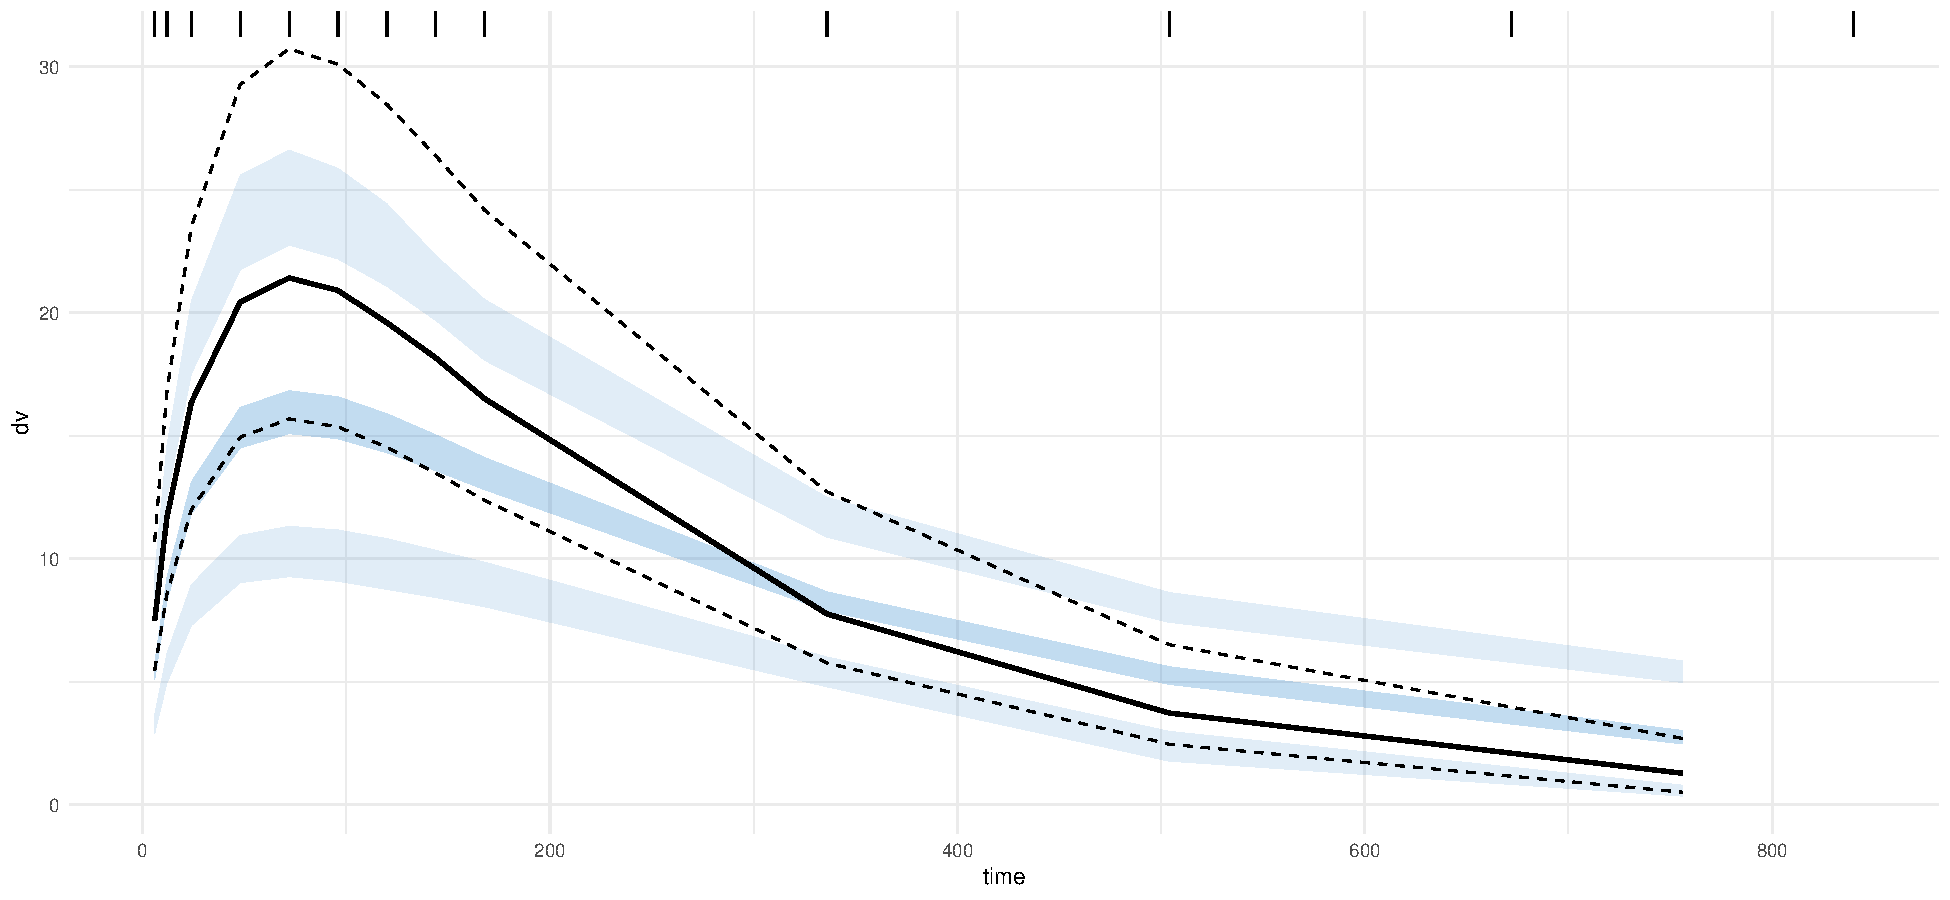
\includegraphics[width=0.9\linewidth]{fig/img/Xpose/vpcPlot.pdf}
    \caption{Enter Caption}
    \label{Fig: VPC}
\end{figure}
A VPC plot is seen in Figure \ref{Fig: VPC}. The plot is constructed from stochastic simulations, usually $n \geq 1000$, from the fitted model. From this simulation, percentiles are plotted versus time. 

Comparing the percentiles from the simulated data with the percentiles from the observed data to aid comparison of the prediction with the observed data. 

When dealing with sparse data less extreme percentiles such as the 75th and 25th percentiles may be more appropriate, as the stochastic component can yield more extreme quantiles. 

In the plot, the light blue are the simulated percentiles, while the darker blue is the simulated median. The dashed lines are the percentiles for the observed data, while the solid line is the median for the observed data. 

As $n \geq 1000$ we get at least $1000$ simulated datasets where the PI are computed. For each simulated dataset, we compute the desired quantiles (for example, the $2.5$th and $97.5$th percentiles) of the simulated observations at each time point. These quantiles will form the lower and upper bounds of the predictive intervals.

A good fit is when the observed median and confidence intervals aligns with the prediction interval and the predicted median. 
% https://www.page-meeting.org/?abstract=1434#:~:text=In%20a%20typical%20VPC%2C%20the,time%20since%20start%20of%20treatment.

\begin{figure}[htbp]
    \centering
    % First 2x2 grid
    \begin{subfigure}[b]{0.45\linewidth}
        \centering
        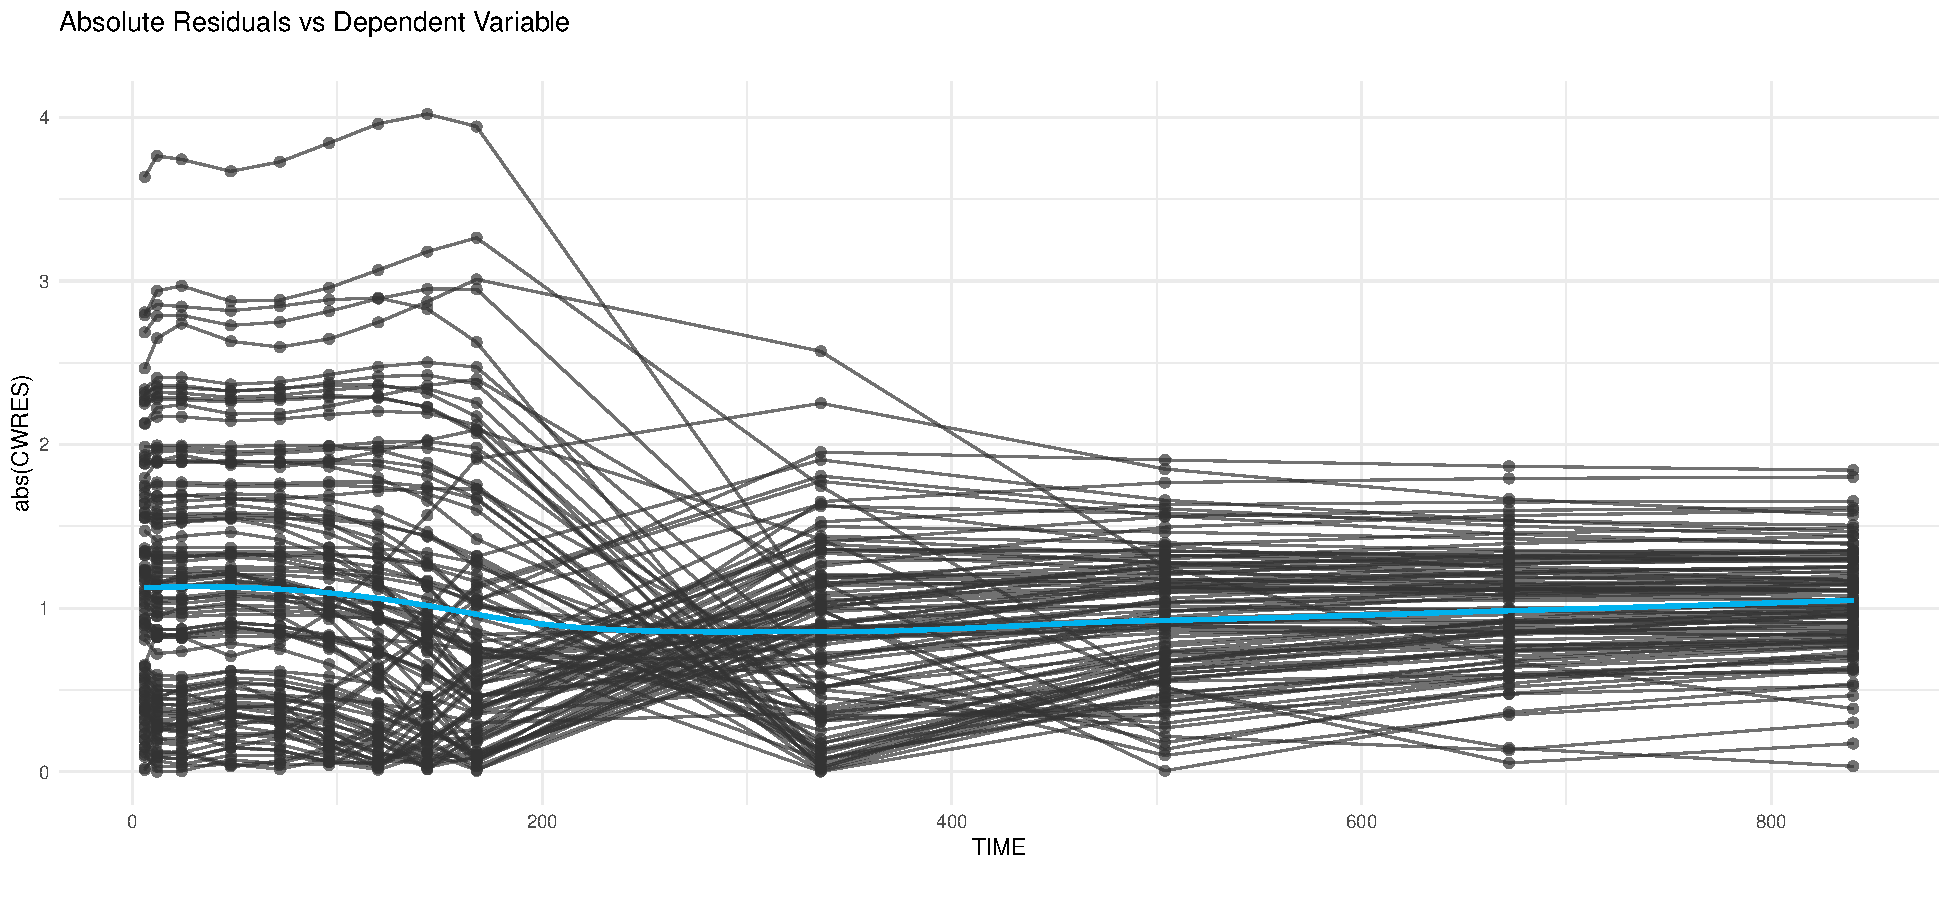
\includegraphics[width=\linewidth]{fig/img/Xpose/absval_res_vs_idv.pdf}
        \caption{absval\_res\_vs\_idv}
        \label{fig:absval_res_vs_idv}
    \end{subfigure}
    \hfill
    \begin{subfigure}[b]{0.45\linewidth}
        \centering
        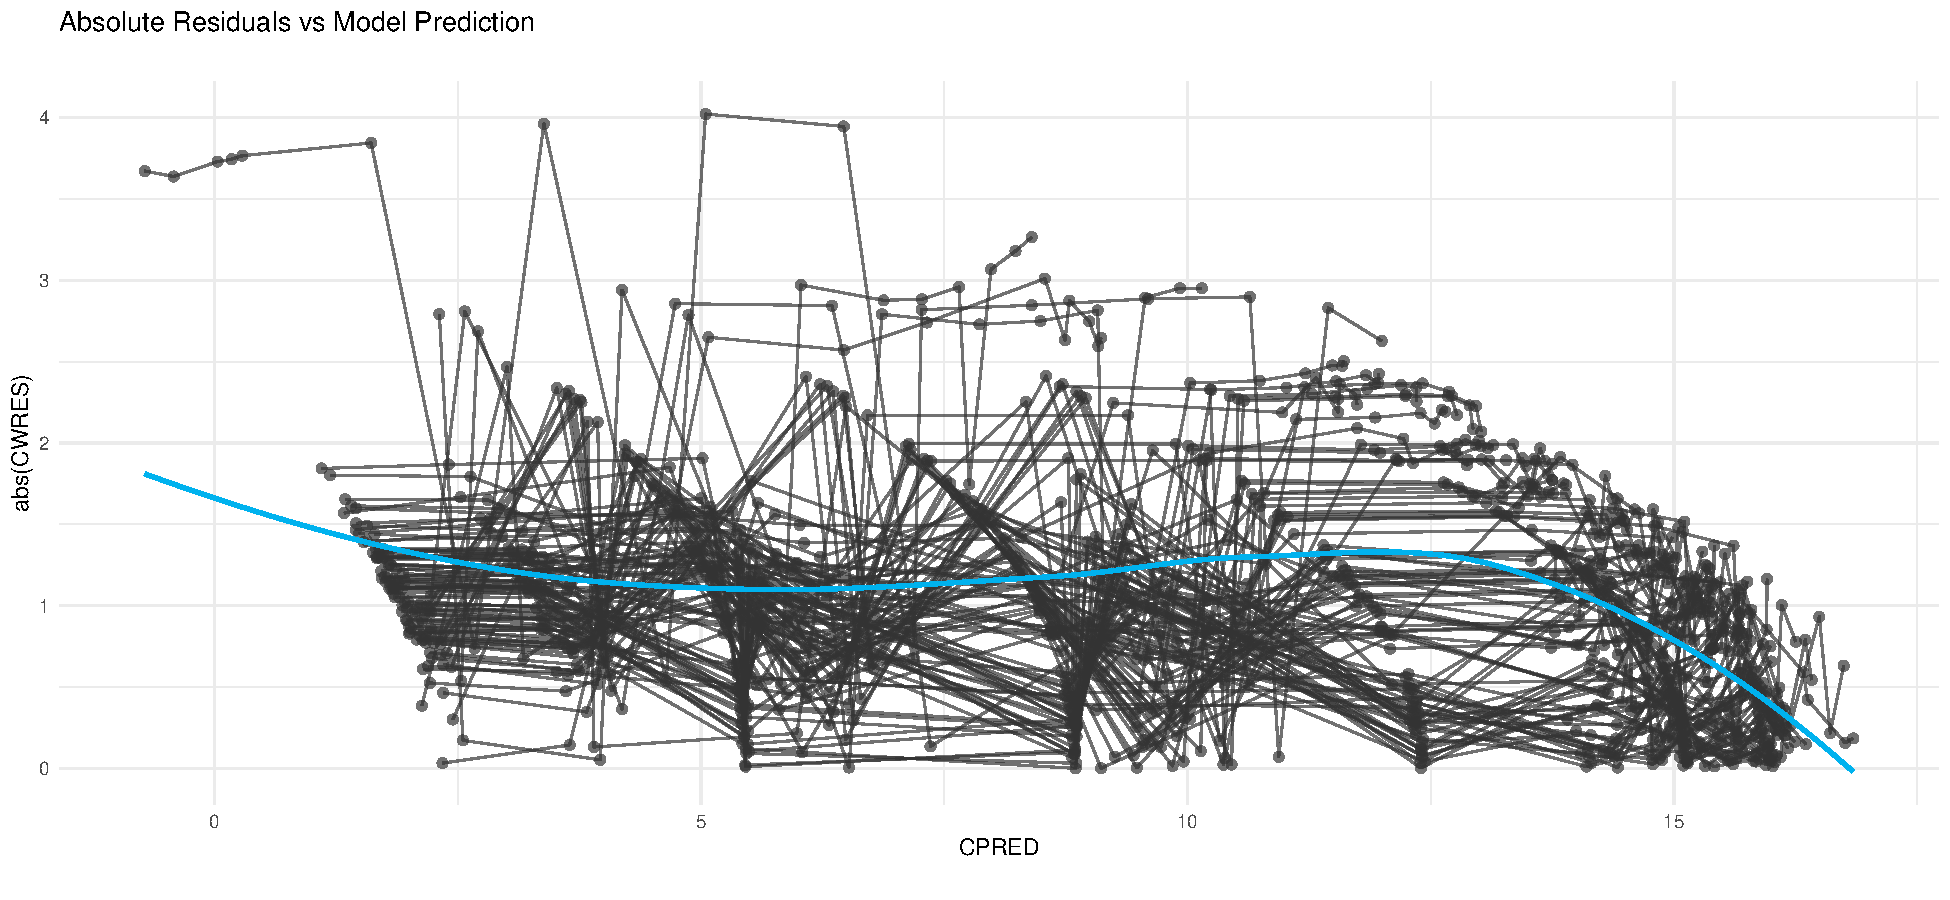
\includegraphics[width=\linewidth]{fig/img/Xpose/absval_res_vs_pred.pdf}
        \caption{absval\_res\_vs\_pred}
        \label{fig:absval_res_vs_pred}
    \end{subfigure}
    
    \vspace{1em} % Adjust vertical space between rows

    \begin{subfigure}[b]{0.45\linewidth}
        \centering
        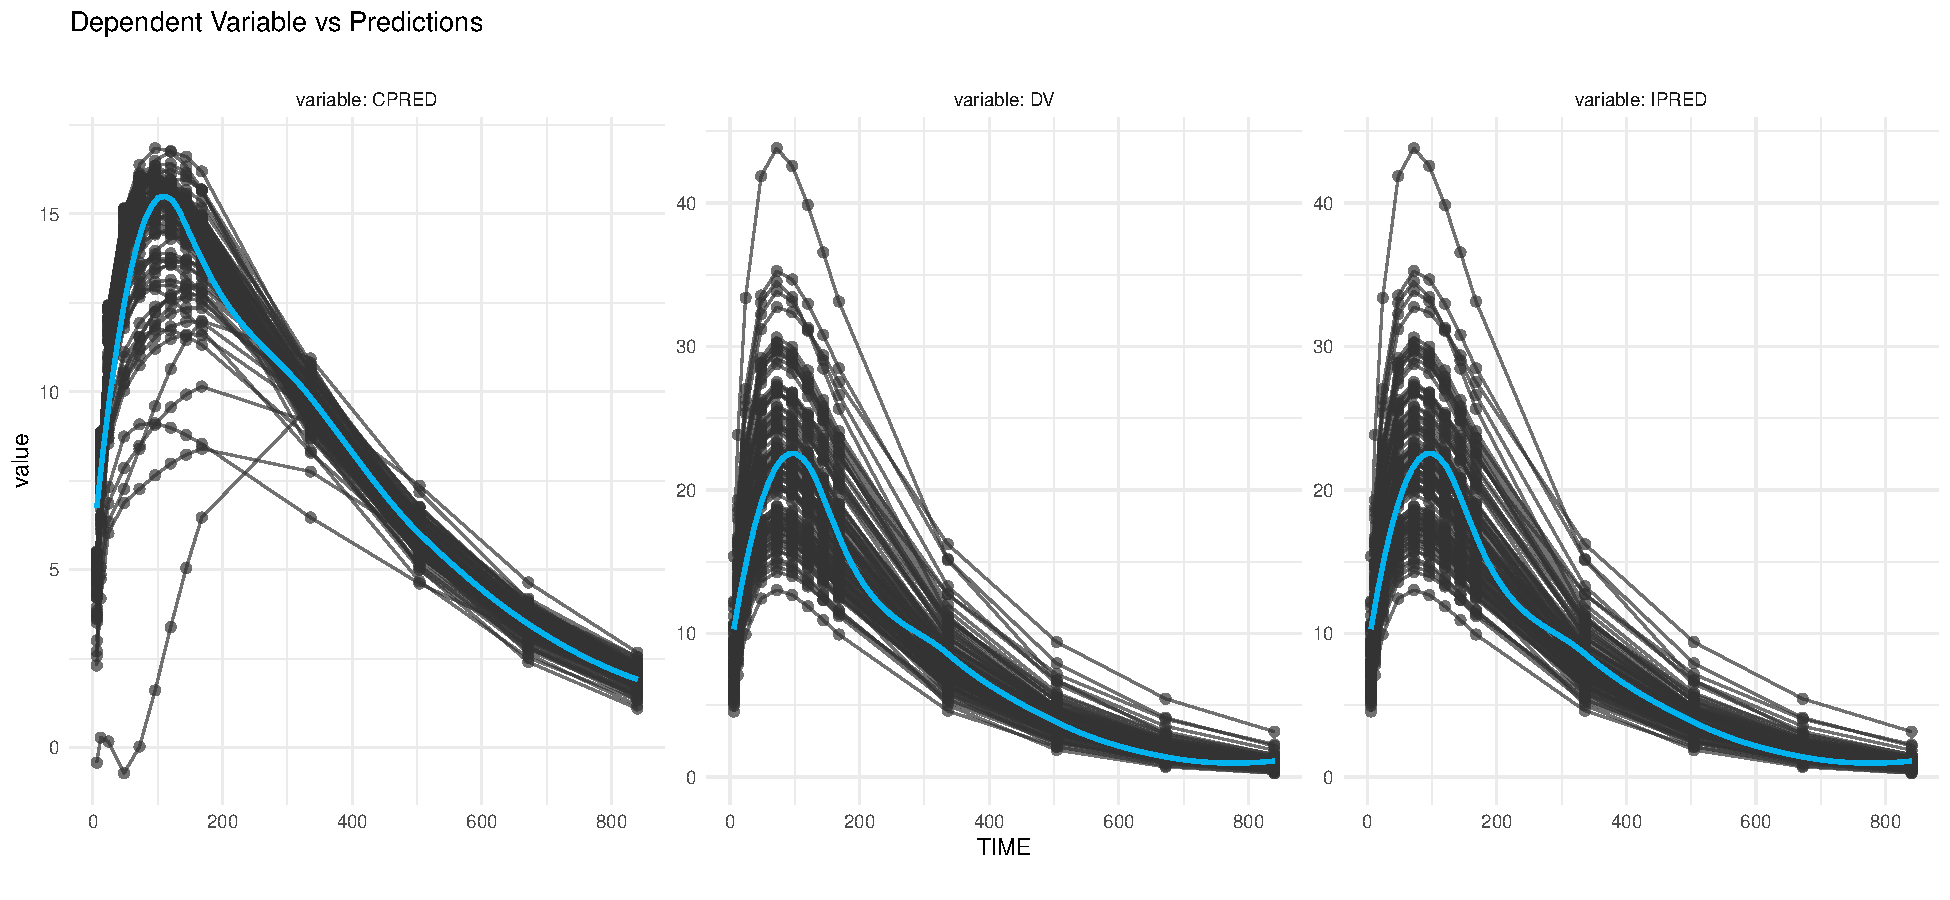
\includegraphics[width=\linewidth]{fig/img/Xpose/dv_preds_vs_idv.pdf}
        \caption{dv\_preds\_vs\_idv}
        \label{fig:dv_preds_vs_idv}
    \end{subfigure}
    \hfill
    \begin{subfigure}[b]{0.45\linewidth}
        \centering
        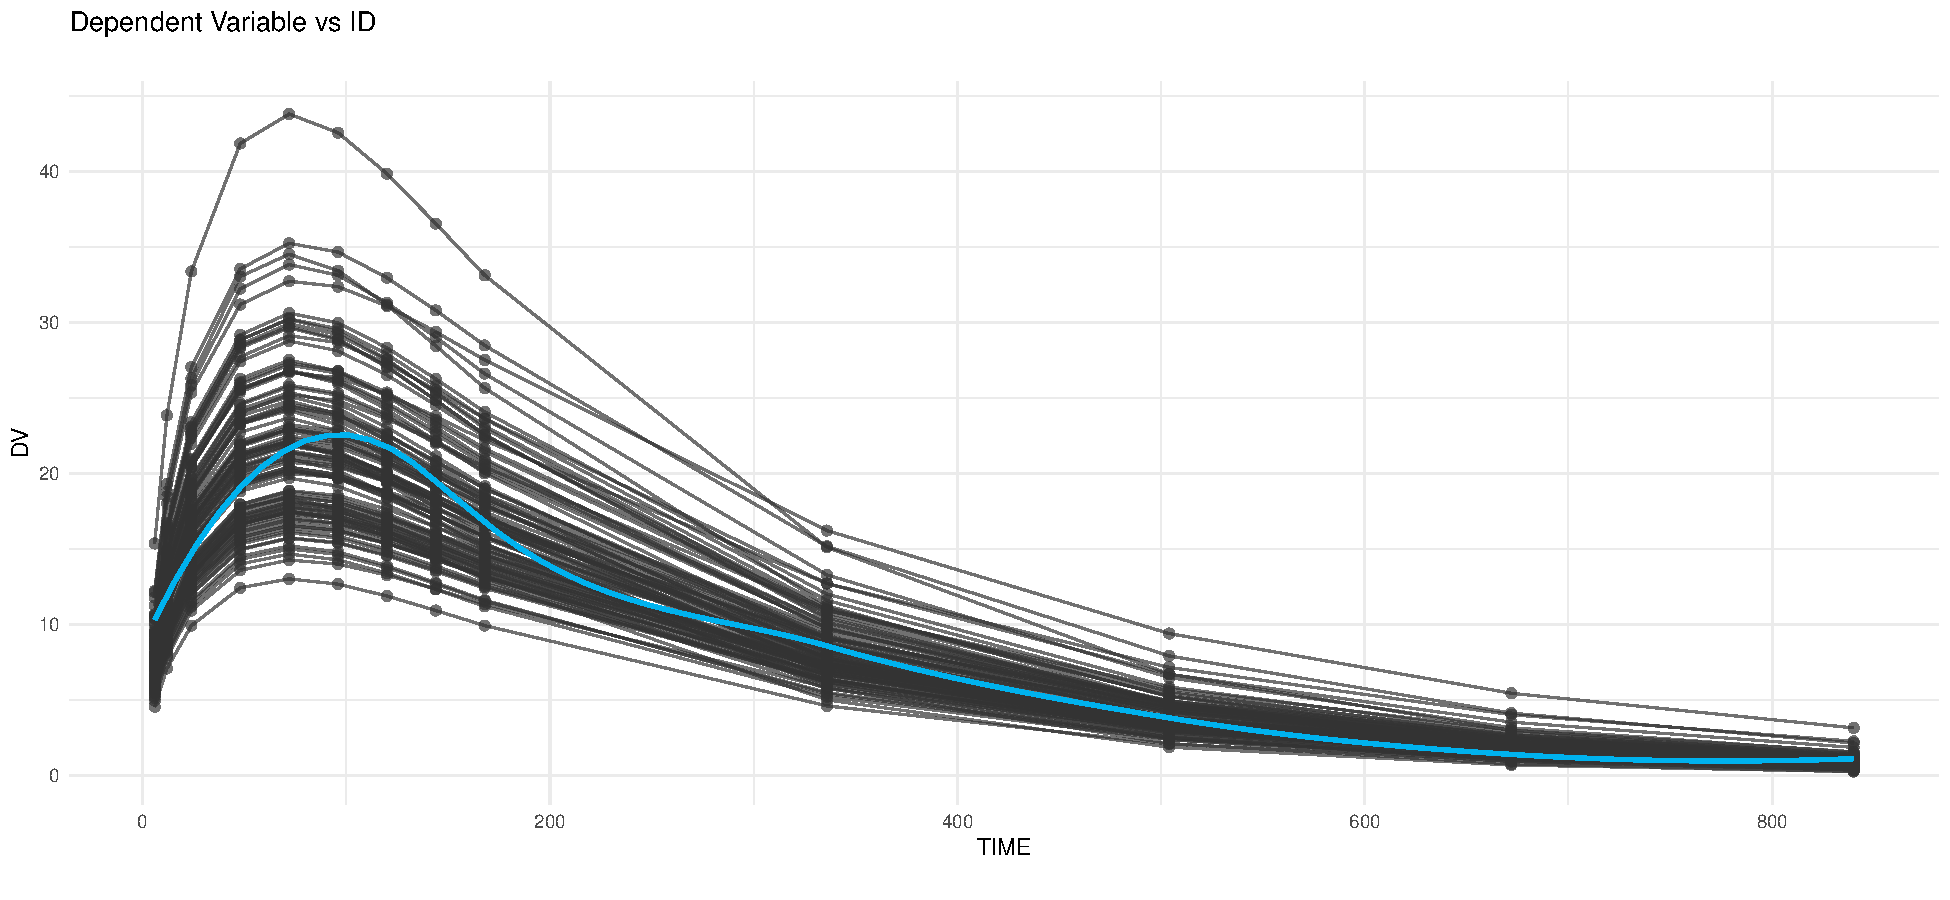
\includegraphics[width=\linewidth]{fig/img/Xpose/dv_vs_idv.pdf}
        \caption{dv\_vs\_idv}
        \label{fig:dv_vs_idv}
    \end{subfigure}

    \vspace{1em}

    % Second 2x2 grid
    \begin{subfigure}[b]{0.45\linewidth}
        \centering
        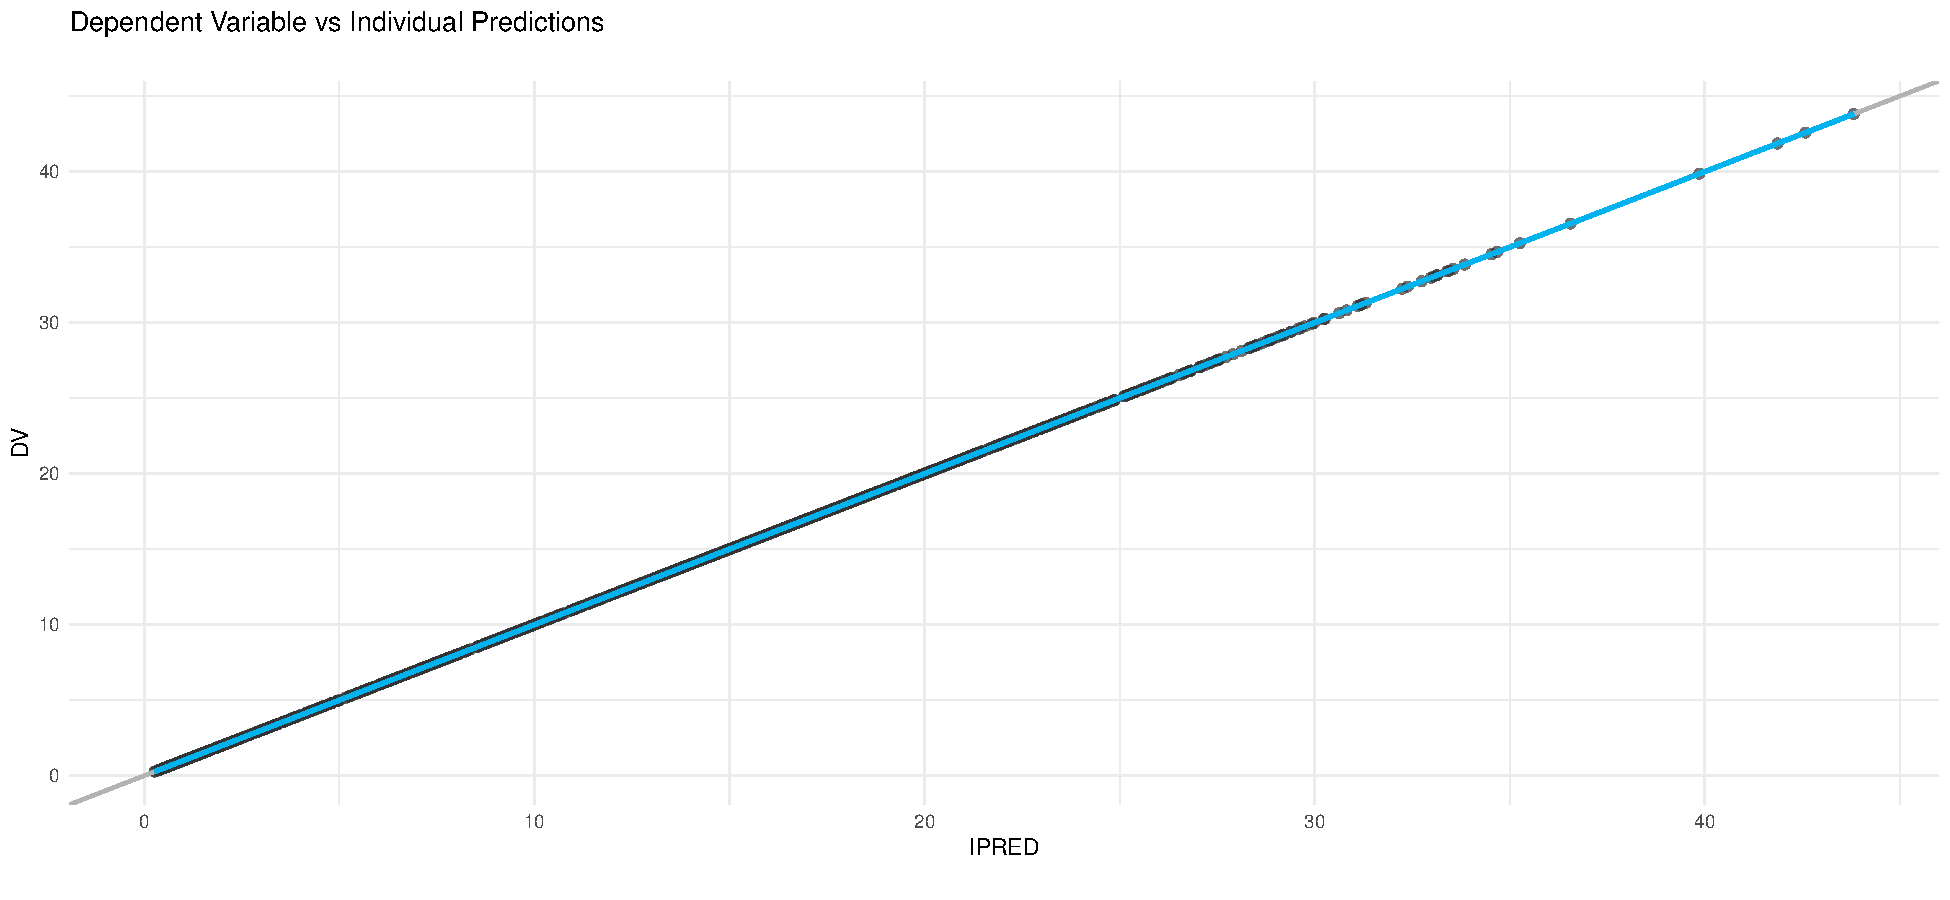
\includegraphics[width=\linewidth]{fig/img/Xpose/dv_vs_ipred.pdf}
        \caption{dv\_vs\_ipred}
        \label{fig:dv_vs_ipred}
    \end{subfigure}
    \hfill
    \begin{subfigure}[b]{0.45\linewidth}
        \centering
        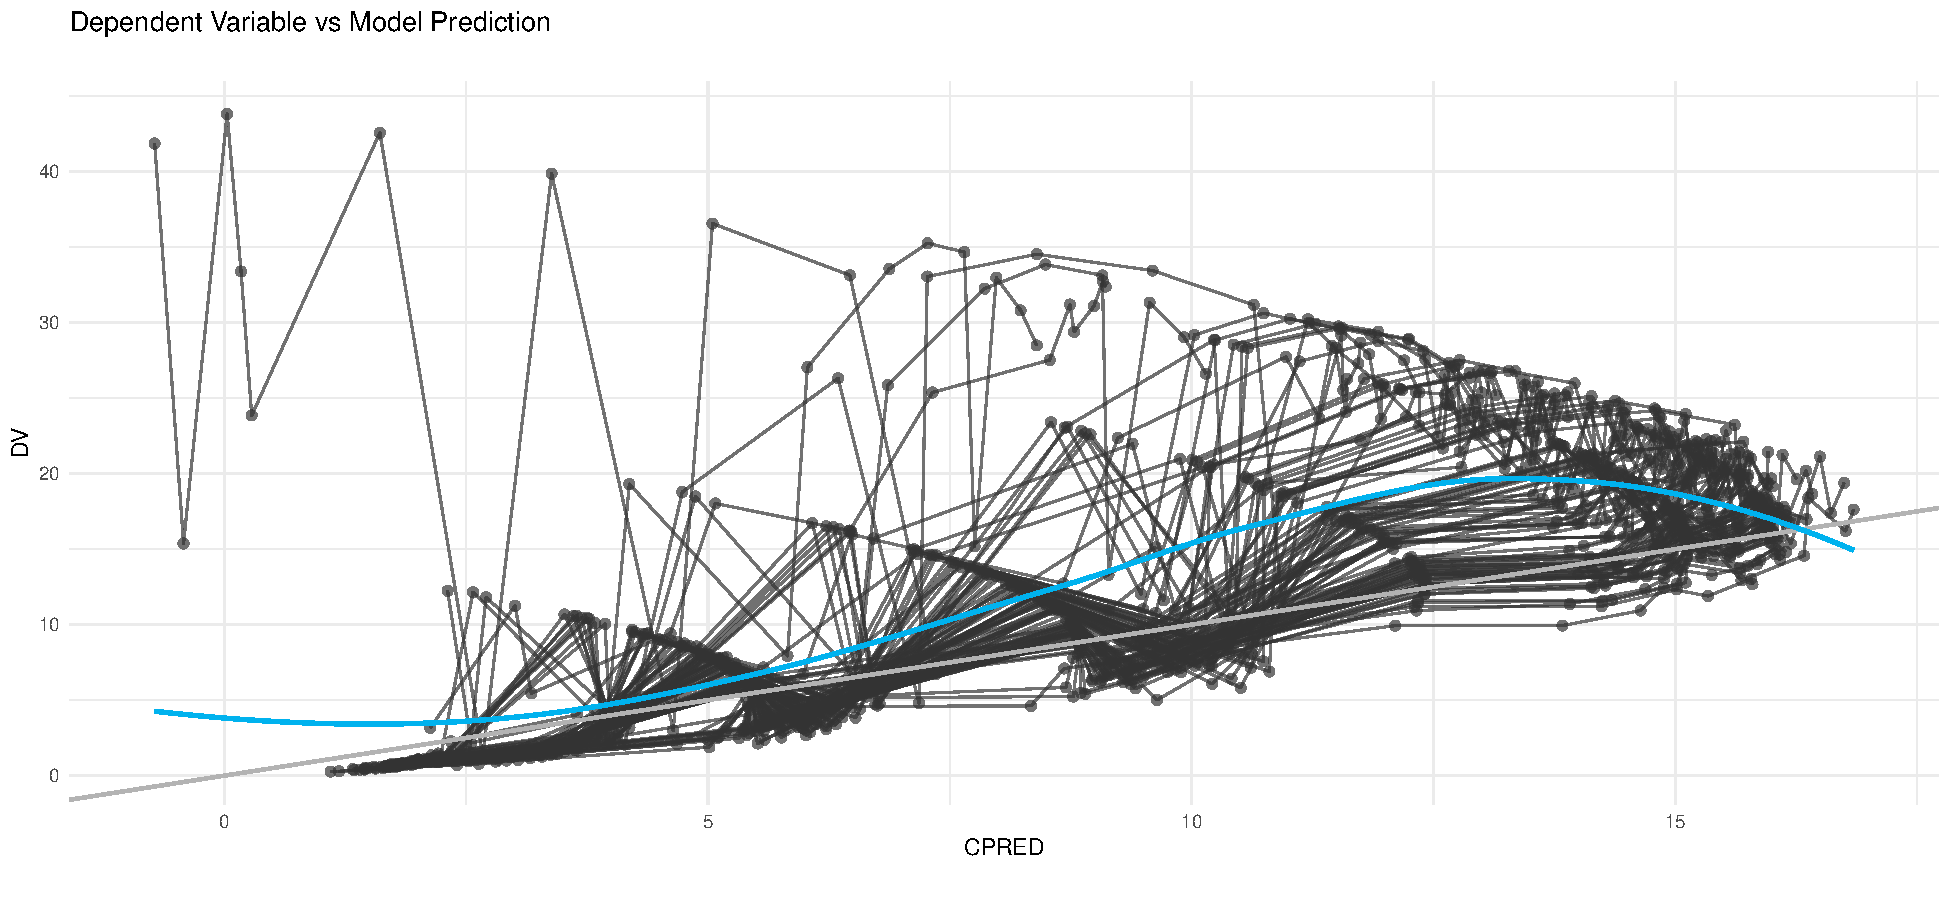
\includegraphics[width=\linewidth]{fig/img/Xpose/dv_vs_pred.pdf}
        \caption{dv\_vs\_pred}
        \label{fig:dv_vs_pred}
    \end{subfigure}

    \vspace{1em}

    % Third 2x2 grid
    \begin{subfigure}[b]{0.45\linewidth}
        \centering
        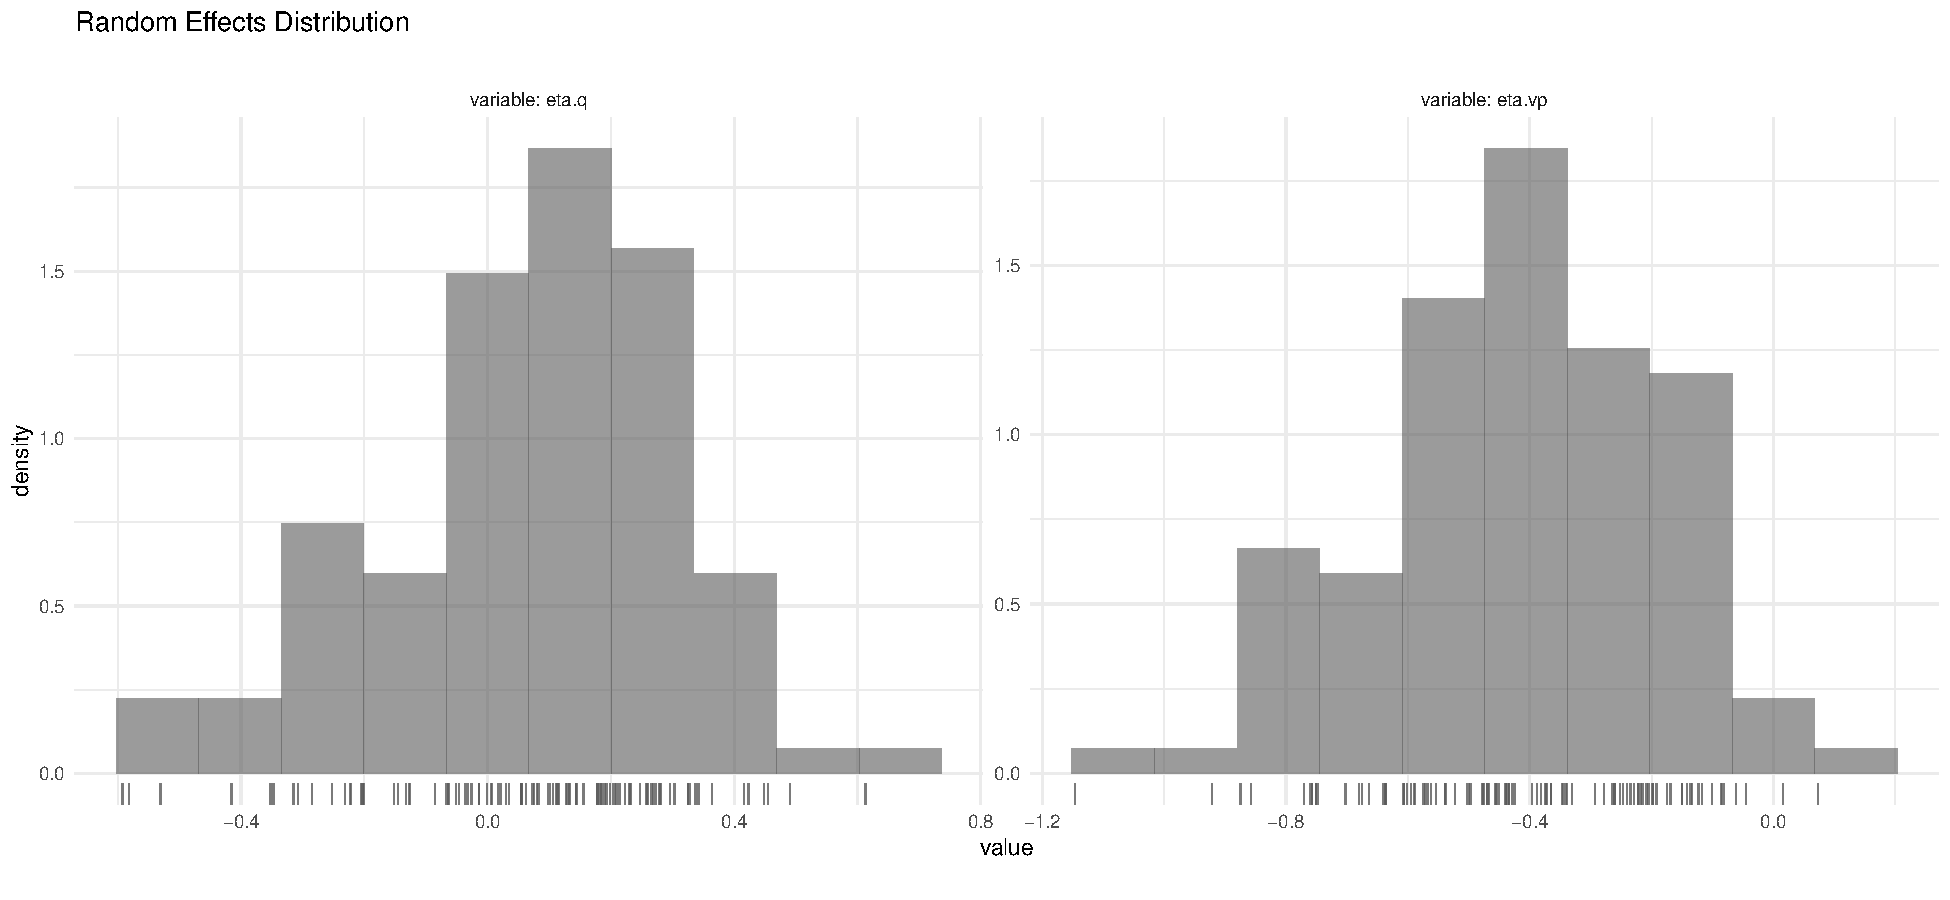
\includegraphics[width=\linewidth]{fig/img/Xpose/eta_distrib.pdf}
        \caption{eta\_distrib}
        \label{fig:eta_distrib}
    \end{subfigure}
    \hfill
    \begin{subfigure}[b]{0.45\linewidth}
        \centering
        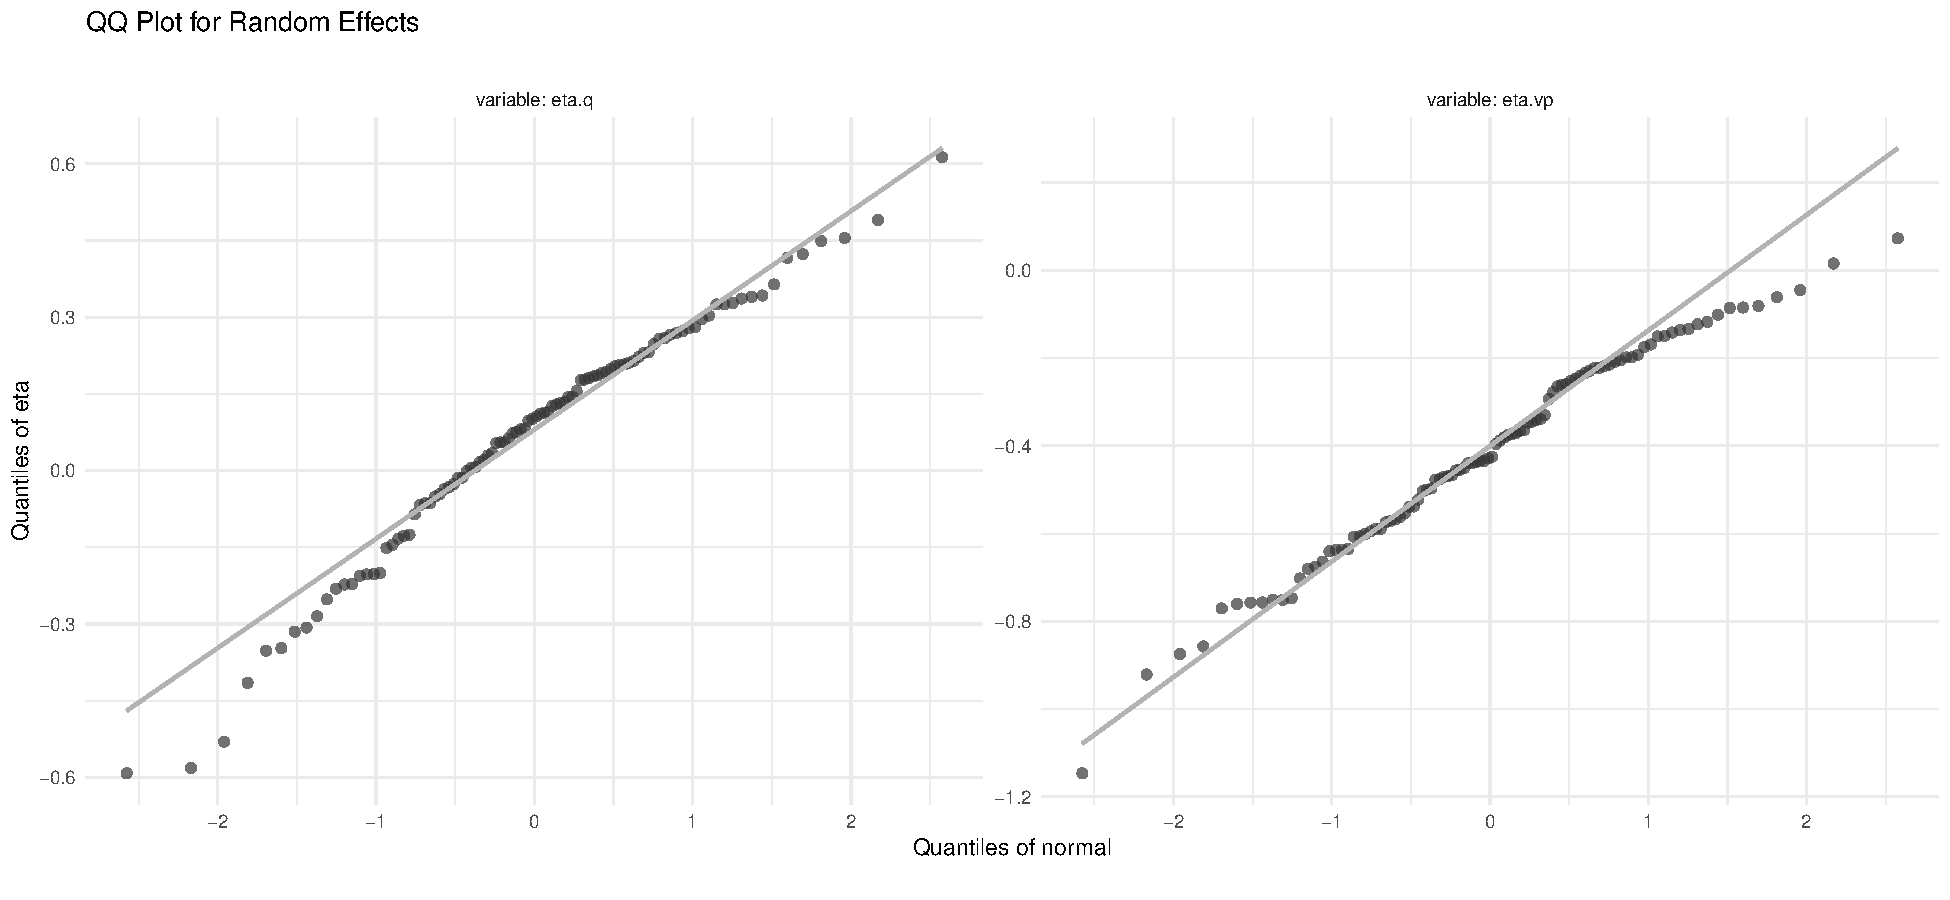
\includegraphics[width=\linewidth]{fig/img/Xpose/eta_qq.pdf}
        \caption{eta\_qq}
        \label{fig:eta_qq}
    \end{subfigure}

    \vspace{1em}

    % Fourth 2x2 grid
    \begin{subfigure}[b]{0.45\linewidth}
        \centering
        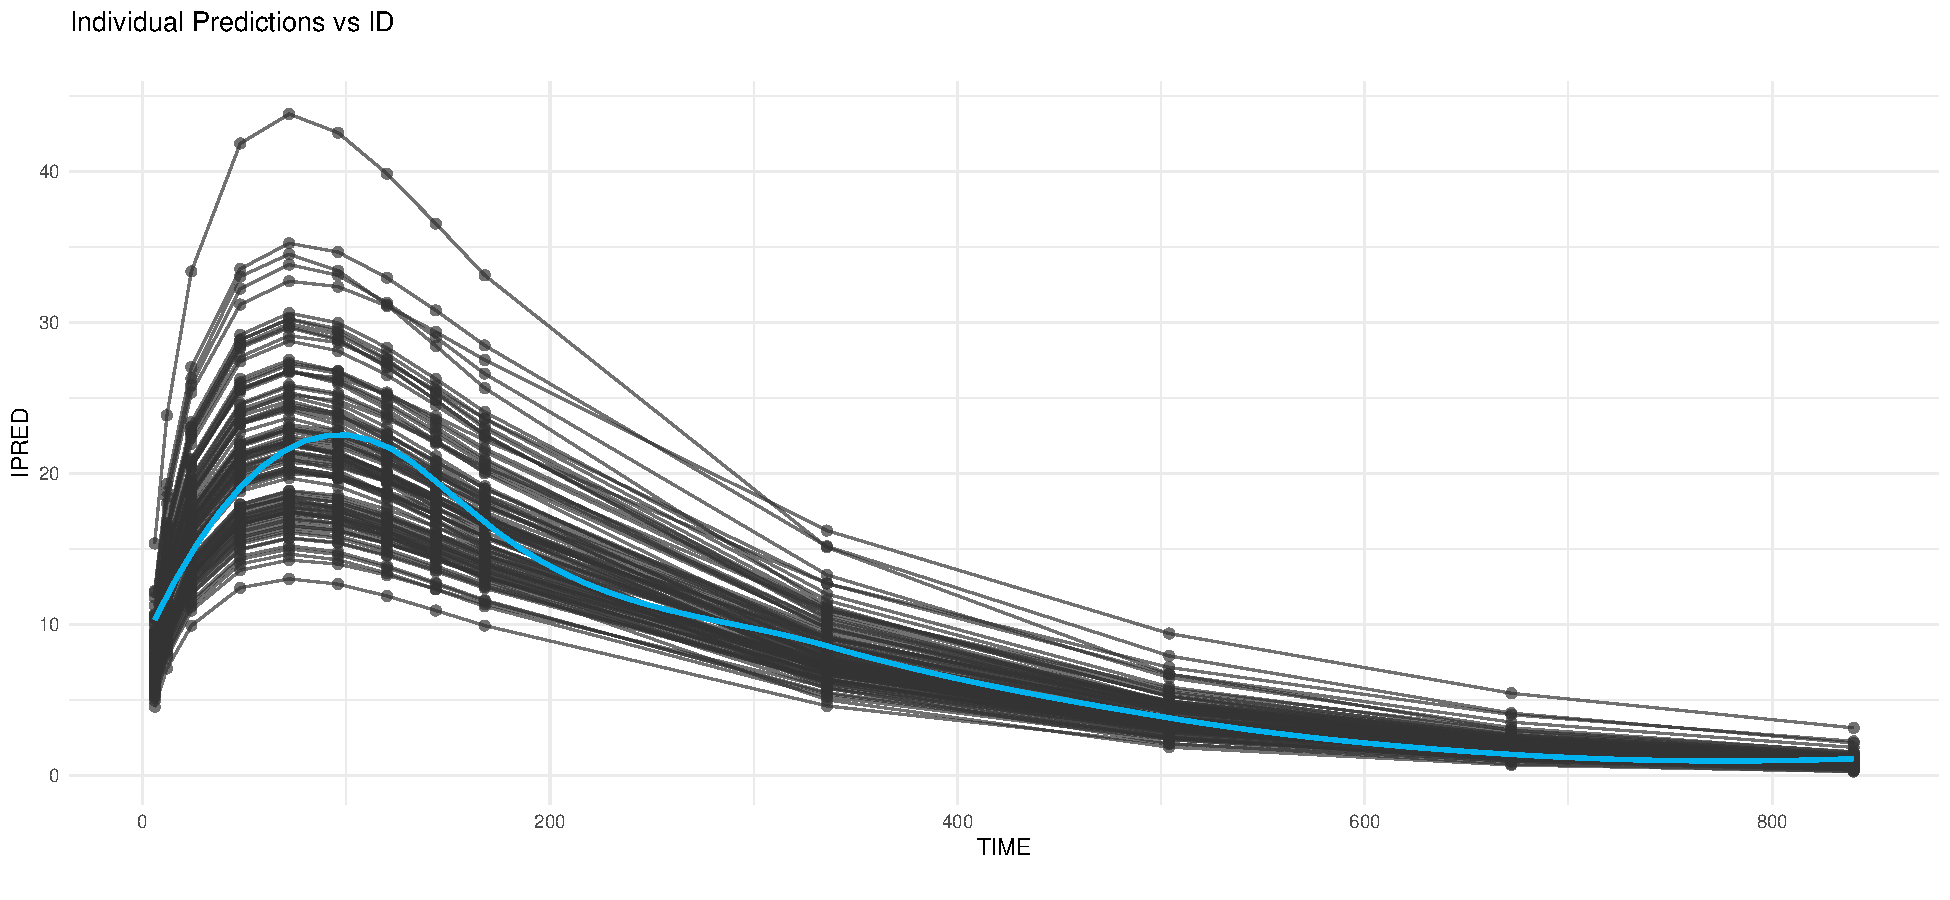
\includegraphics[width=\linewidth]{fig/img/Xpose/ipred_vs_idv.pdf}
        \caption{ipred\_vs\_idv}
        \label{fig:ipred_vs_idv}
    \end{subfigure}
    \hfill
    \begin{subfigure}[b]{0.45\linewidth}
        \centering
        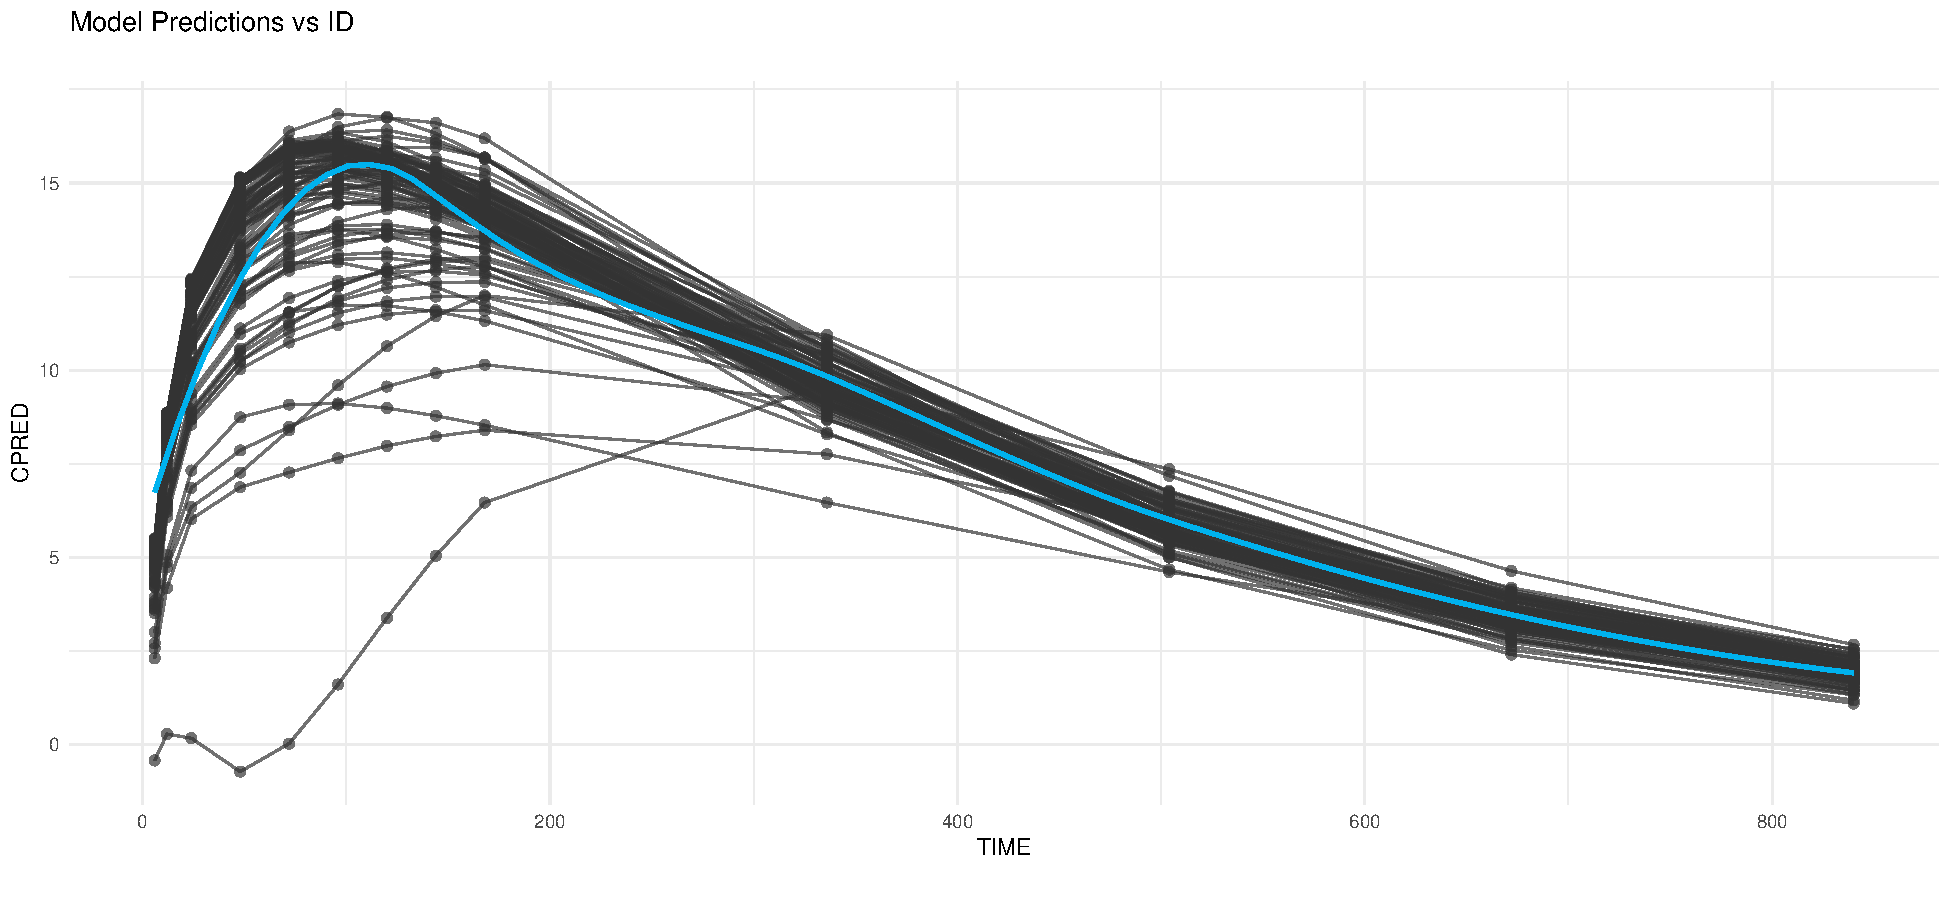
\includegraphics[width=\linewidth]{fig/img/Xpose/pred_vs_idv.pdf}
        \caption{pred\_vs\_idv}
        \label{fig:pred_vs_idv}
    \end{subfigure}

    \vspace{1em}

    % Fifth 2x2 grid
    \begin{subfigure}[b]{0.45\linewidth}
        \centering
        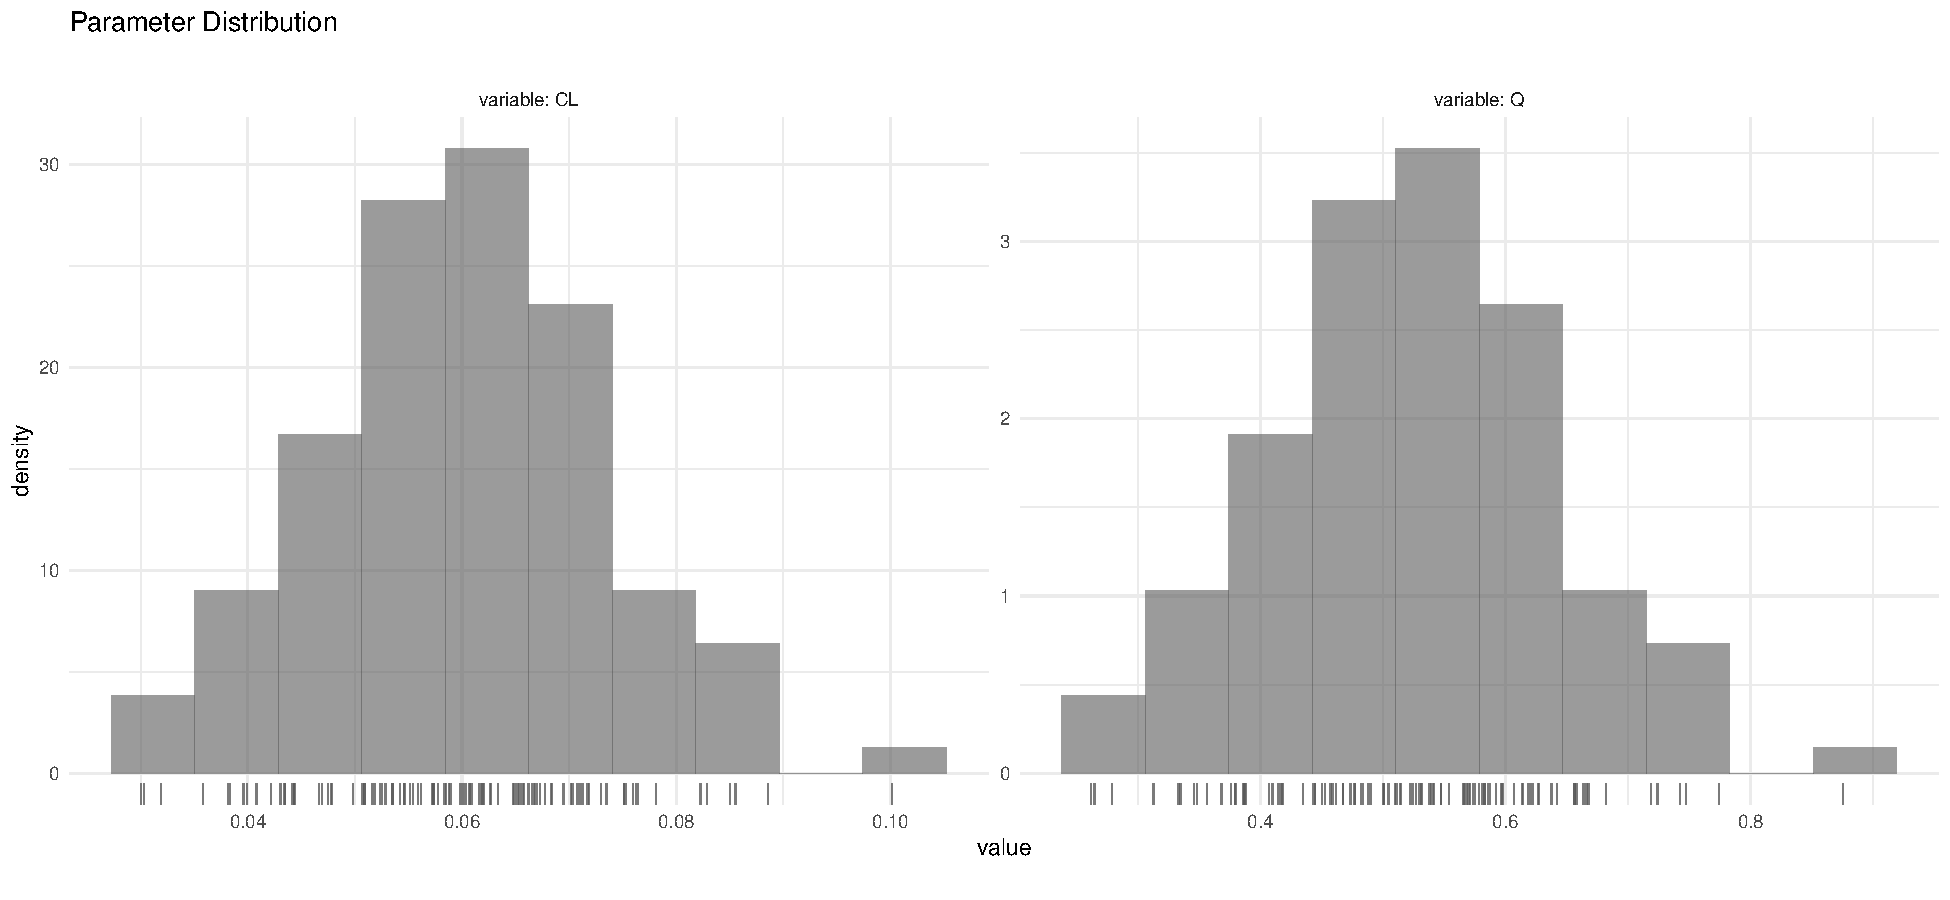
\includegraphics[width=\linewidth]{fig/img/Xpose/prm_distrib.pdf}
        \caption{prm\_distrib}
        \label{fig:prm_distrib}
    \end{subfigure}
    \hfill
    \begin{subfigure}[b]{0.45\linewidth}
        \centering
        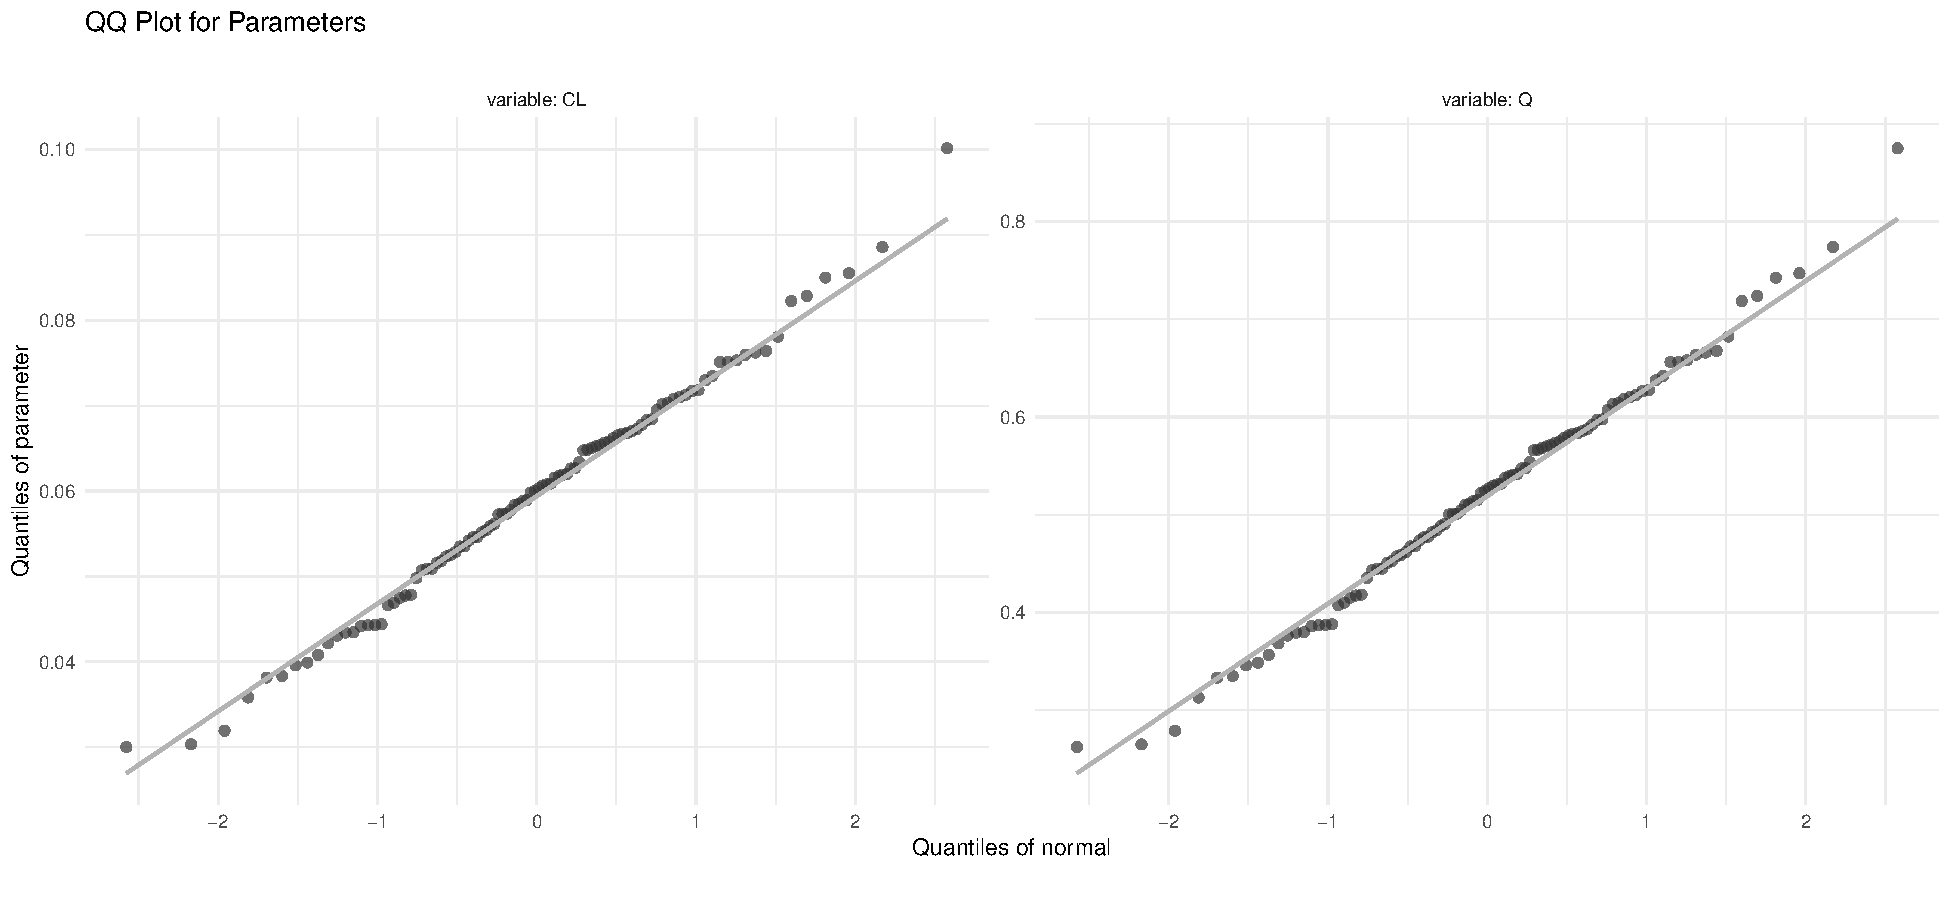
\includegraphics[width=\linewidth]{fig/img/Xpose/prm_qq.pdf}
        \caption{prm\_qq}
        \label{fig:prm_qq}
    \end{subfigure}
\end{figure}




\begin{figure}
\centering
    % Sixth 2x2 grid
    \begin{subfigure}[b]{0.45\linewidth}
        \centering
        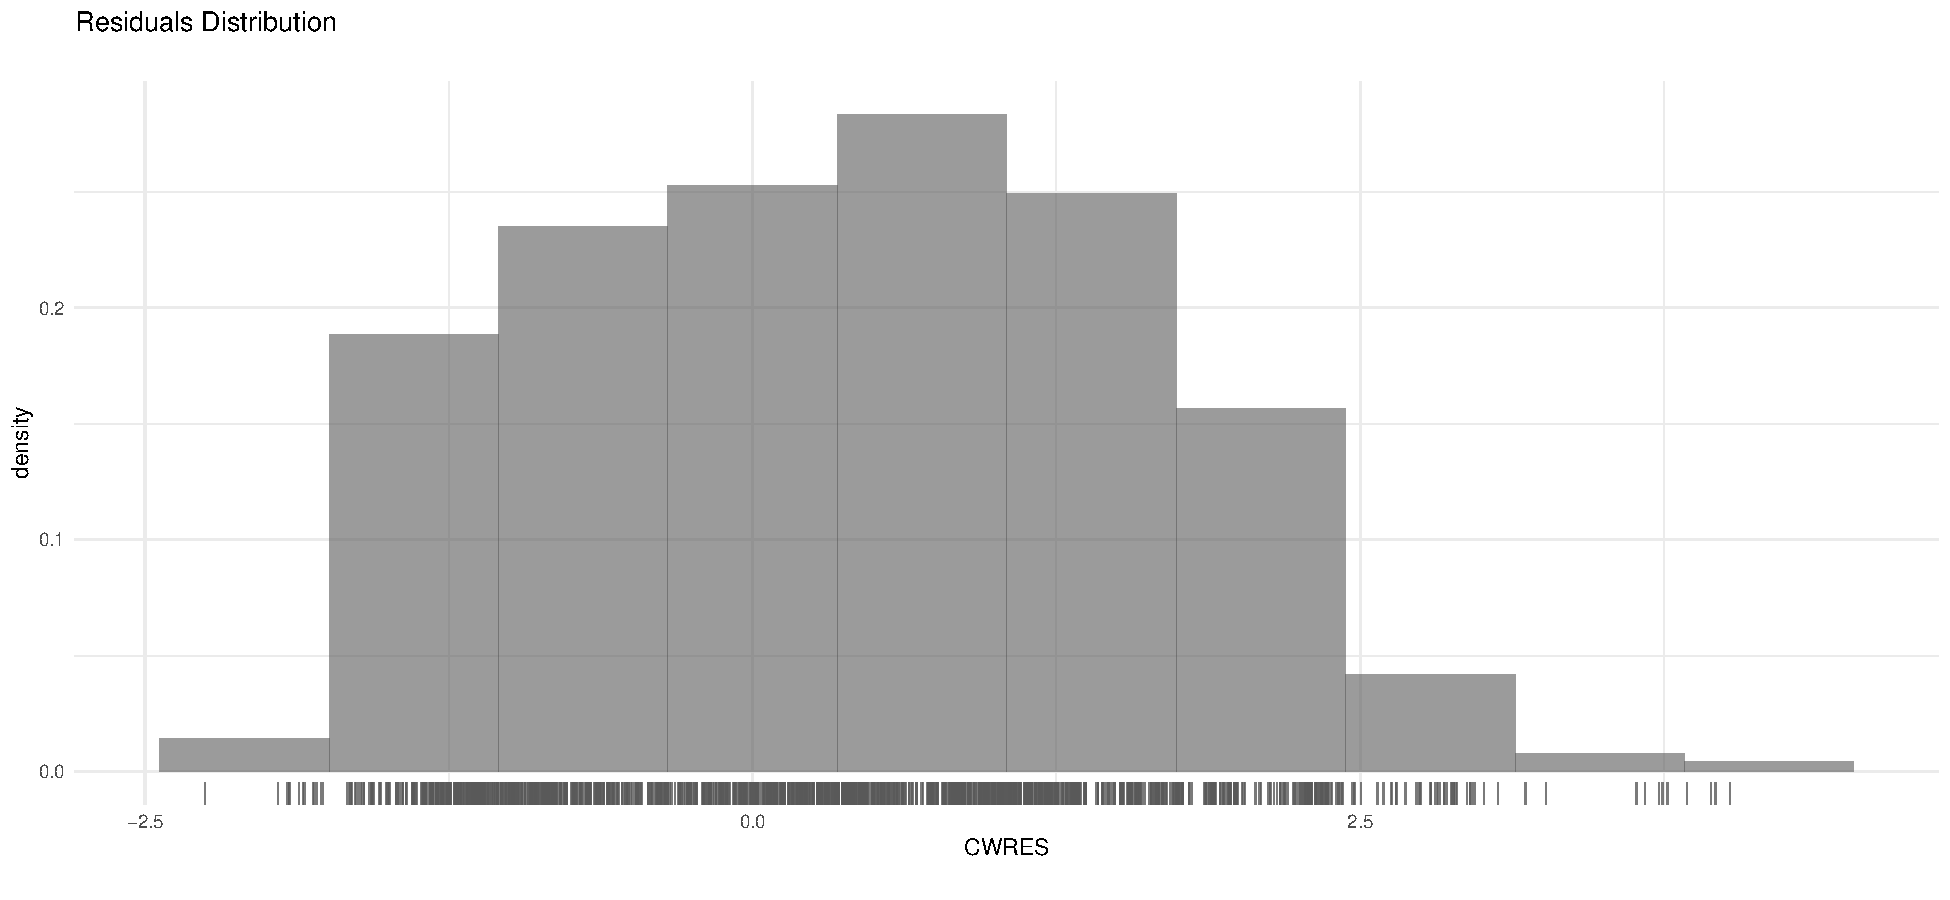
\includegraphics[width=\linewidth]{fig/img/Xpose/res_distrib.pdf}
        \caption{res\_distrib}
        \label{fig:res_distrib}
    \end{subfigure}
    \hfill
    \begin{subfigure}[b]{0.45\linewidth}
        \centering
        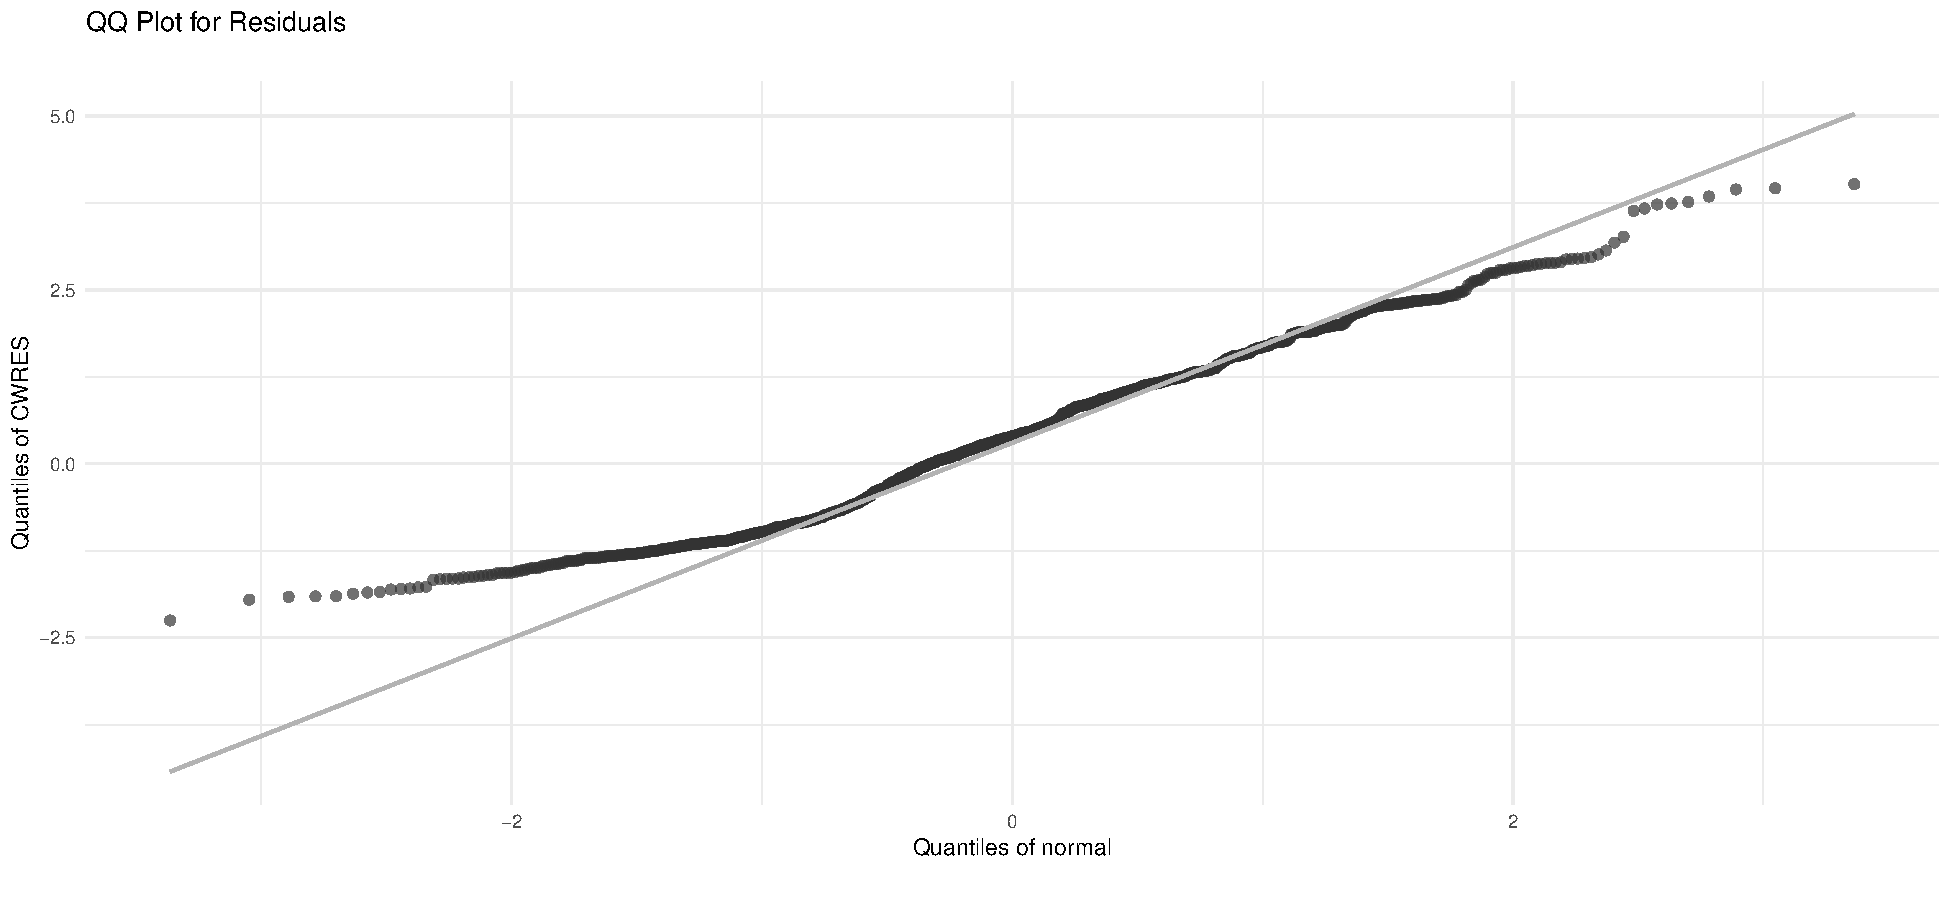
\includegraphics[width=\linewidth]{fig/img/Xpose/res_qq.pdf}
        \caption{res\_qq}
        \label{fig:res_qq}
    \end{subfigure}

    \vspace{1em}

    % Seventh 2x2 grid
    \begin{subfigure}[b]{0.45\linewidth}
        \centering
        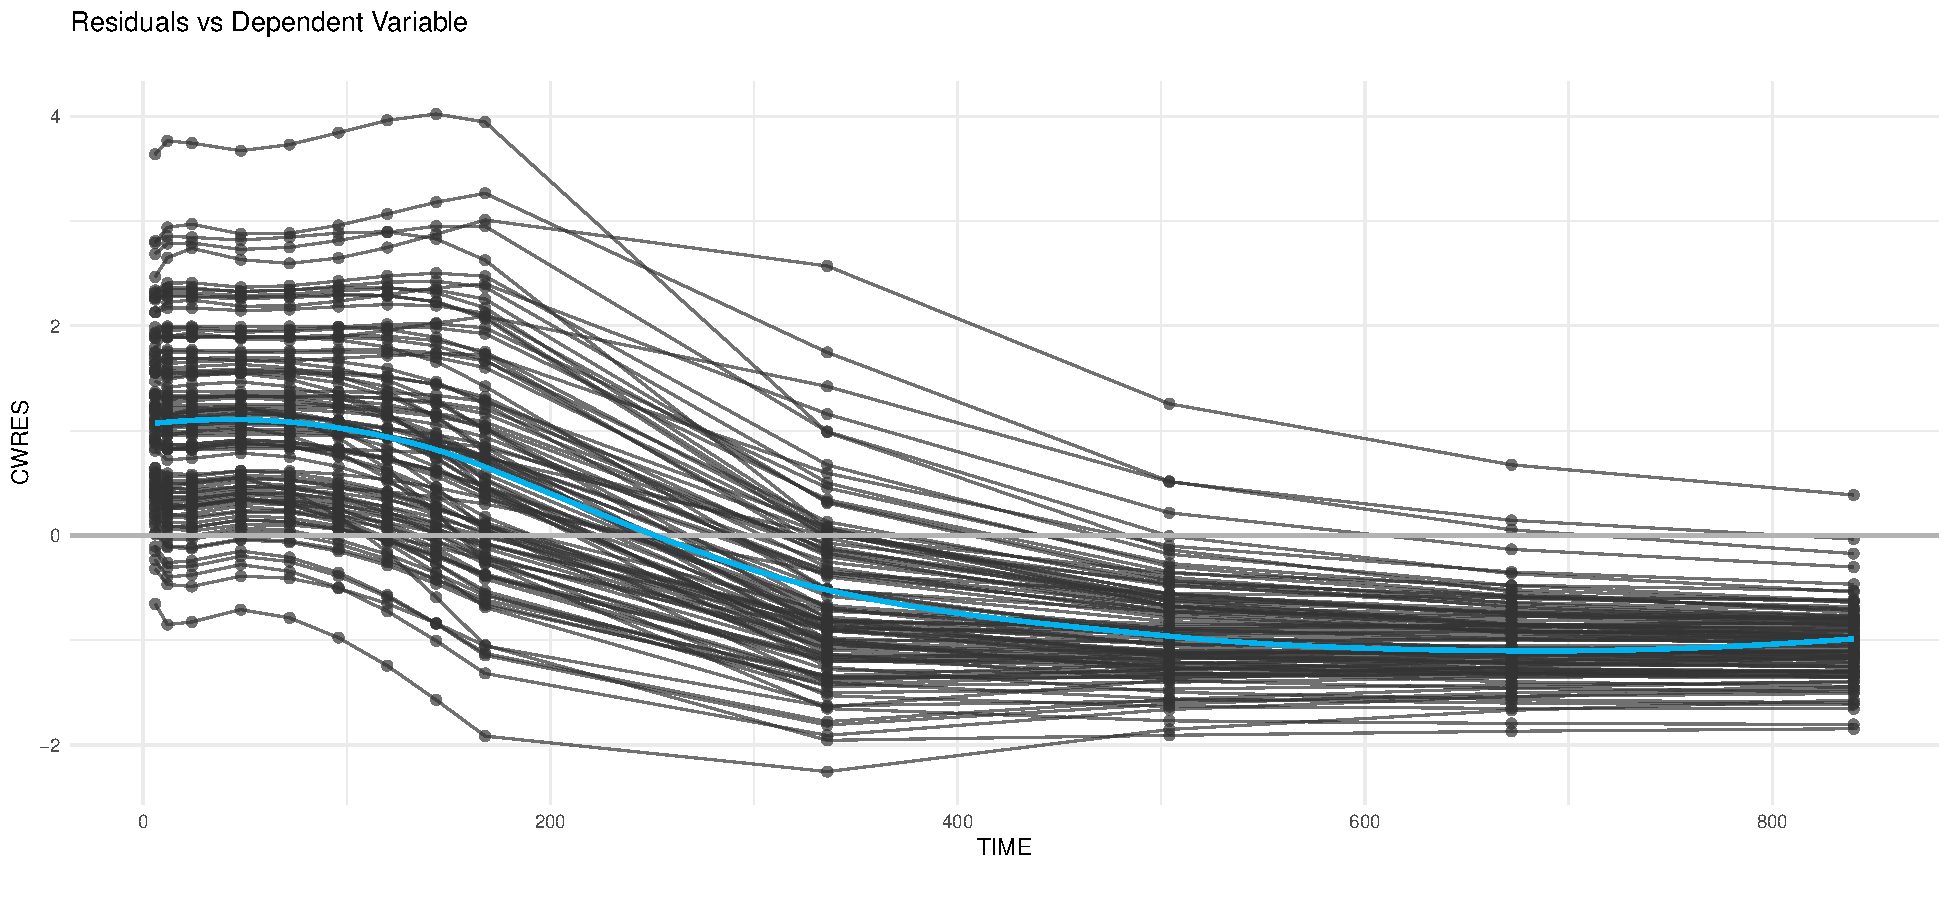
\includegraphics[width=\linewidth]{fig/img/Xpose/res_vs_idv.pdf}
        \caption{res\_vs\_idv}
        \label{fig:res_vs_idv}
    \end{subfigure}
    \hfill
    \begin{subfigure}[b]{0.45\linewidth}
        \centering
        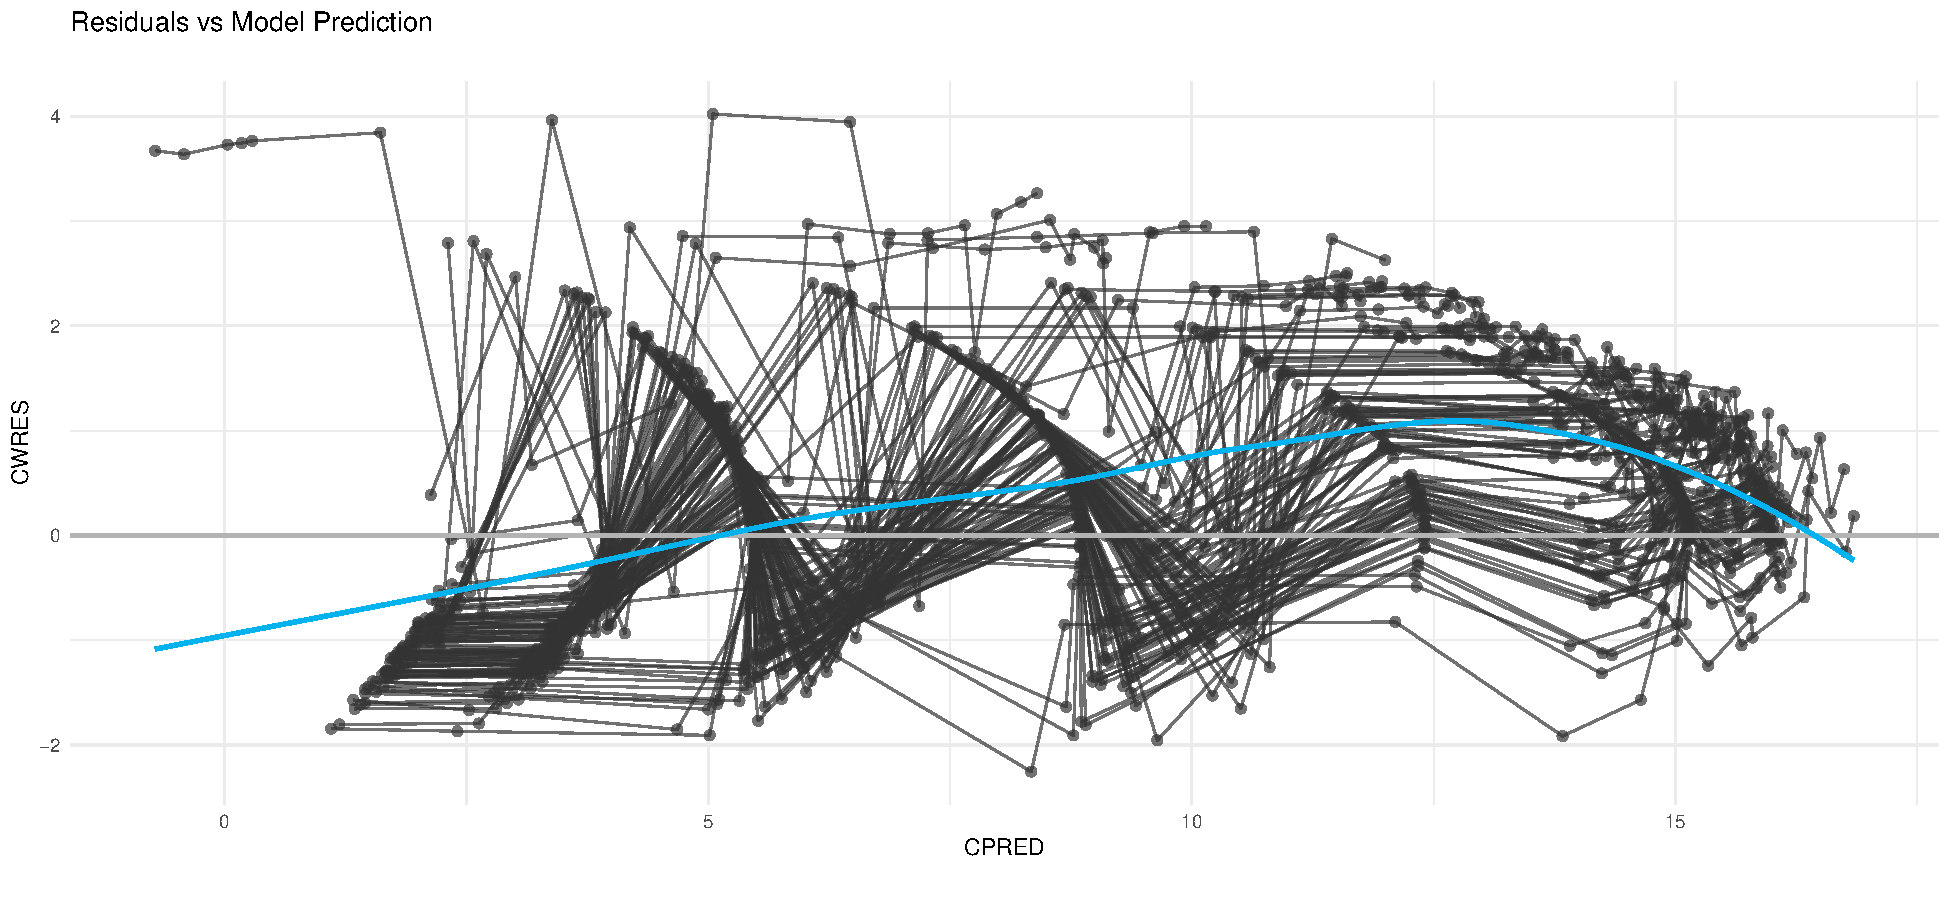
\includegraphics[width=\linewidth]{fig/img/Xpose/res_vs_pred.pdf}
        \caption{res\_vs\_pred}
        \label{fig:res_vs_pred}
    \end{subfigure}

    \caption{Main caption for the figures}
    \label{fig:all_figures}
\end{figure}
% KILDE: Conditional Weighted Residuals (CWRES): A Model Diagnostic - DOI: 10.1007/s11095-007-9361-x
% for the FOCE Method
Firstly, WRES, CWRES, pred, Ipred, dv, and IDV will be explained, as these are used to diagnostic the models. 

The weighted residuals (WRES) are computed as
\begin{align*}
    \text{WRES} = \frac{y_i - \Ex{y_i}_{FO}}{\sqrt{\Cov{y_i}_{FO}}}
\end{align*}

The conditional weighted residuals (CWRES) are computed as
\begin{align*}
    \text{CWRES} = \frac{y_i - \Ex{y_i}_{FOCE}}{\sqrt{\Cov{y_i}_{FOCE}}}
\end{align*}










\chapter{pure yap}
\begin{itemize}
    \item Relationship between explanatory- and response variables is not required to be linear.
    \item Inclusion of random effects in non-linear framework results in the absence of a closed form expression for the likelihood function - this implies we have to use methods to approximate the likelihood function
    \item Approximation methods
    \item HOW TO BUILD POP-PK-MODEL: See Bonate p. 263 - modelbygningen opdeles i fem steps (har forkortet dem ned her):
    \begin{enumerate}
        \item Determine the structual PK model (ligesom vi gør i preliminary) and estimate the model without covariates
        \item Examine the assumptions regarding the distribution of random effects
        \item Select covariates for inclusion in the model (covariate screening)
        \item Build the model using covariates (redundant if the covariates were tested directly in the NLME model)
        \item Evaluate final parameter estimates - test assumptions to validate the model
    \end{enumerate}
    \item If the primary goal of this project is to make simulation studies to estimate PK parameters given a specific structural PK model in which the relationship with the covariates is known, our task is now to formalize how to build such a model. All that has to do with model verification is much less relevant since we know the true model.
    \item AIM: Determine the structural PK model and use a given model for the covariates and then estimate the model with several estimation methods and then compare with the exact same models estimated using NONMEM.
\end{itemize}
We want to allow for individual variability for the PK parameters. An an example we might want to model the elimination rate as
\begin{align*}
    K_{e,i}=K_{e,pop}\left(\frac{\text{covariate}_i}{\text{ covariate}_{pop}}\right)^{\alpha}\exp({\eta_{K_{e,i}}}), 
\end{align*}
where $K_{e,i}$ is the elimination rate for subject $i$, $K_{e,pop}$ is the population mean for $K_{e}$, $\eta_{K_{e,i}} \sim N(0, \omega^2)$ is the subject variability, and $\alpha$ is a constant indicating the influence of the covariate.


\section{Modelopbygning}
\begin{align*}
    y_i &= (y_{1,i},\dots,y_{1,n_i})^\top \in \R^{n_i}\\
    Y&=(y_1,y_2,\dots,y_N)^\top= (y_{1,1},\dots,y_{1,n_1},y_{2,1},\dots,y_{2,n_2},\dots,y_{N,1},\dots,y_{N,n_N})^\top \in \R^{n_1+n_2+\cdots+n_N}\\
    G(t,u,\theta)&=(g_1(\theta_1),g_2(\theta_2),\dots,g_N(\theta_N))^\top \in \R^{n_1+n_2+\cdots+n_N}\\
    \epsilon &= (e_1,e_2,\dots,e_N)^\top=(e_{1,1},\dots,e_{1,n_1},e_{2,1},\dots,e_{2,n_2},\dots,e_{N,1},\dots,e_{N,n_N})^\top \in \R^{n_1+n_2+\cdots+n_N}\\
    Y &= G(t,u,\theta) + \epsilon\\
    \theta &= [(h(a_1,\beta,\eta_1),h(a_2,\beta, \eta_2), \dots,h(a_N,\beta,\eta_N)]^\top \in \R^{pN}\\
    e_{i,j} &\sim (0,\sigma^2)\\
    e_i &\sim (0,R_i), R_i \in \R^{n_i \times n_i}\\
    \eta_i &\sim (0,\Omega), \Omega \in \R^{r \times r}\\
    \eta &= (\eta_{1,1},\eta_{1,2},\dots,\eta_{1,N},\dots,\eta_{r,1},\dots,\eta_{r,N})=  (\eta_1,\dots,\eta_N)^\top \in \R^{rN}\\
    \eta &\sim (0,\Sigma)\\
    \Sigma &=
\begin{bmatrix}
    \Omega & O & \cdots & O \\
    O & \Omega & \cdots & O \\
    \vdots & \vdots & \ddots & \vdots \\
    O & O & \cdots &\Omega
\end{bmatrix}
 \in \R^{rN \times rN}\\
     R &=
\begin{bmatrix}
    R_1 & O & \cdots & O \\
    O & R_2 & \cdots & O \\
    \vdots & \vdots & \ddots & \vdots \\
    O & O & \cdots & R_N
\end{bmatrix}
 \in \R^{(n_1+n_2+\dots+n_N)\times (n_1+n_2+\dots+n_N)}\\
 \Omega &= \begin{bmatrix}
    \omega_{1,1} & \omega_{1,2} & \cdots & \omega_{1,r} \\
    \omega_{2,1} & \omega_{2,2} & \cdots & \omega_{2,r} \\
    \vdots & \vdots & \ddots & \vdots \\
    \omega_{r,1} & \omega_{r,2} & \cdots & \omega_{r,r}
\end{bmatrix}, \quad \omega_{k,m} = \Cov{\eta_{i,k},\eta_{i,m}}.
\end{align*}

% \section{Residual variance models}
% %Bonat side 243
% The variability that remains unexplained by a NLME-model is referred to as the residual variance. This residual variance is explicitly represented as the error term in the first stage of an NLME-model, represented in \eqref{eq: NLME Stage 1}, and can be modeled with a residual variance model. As the residual variance becomes larger or more heterogeneous, it becomes increasingly more important to include a residual variance model to the overall model. In \eqref{eq: NLME Stage 1}, the error term is added to the non-linear function, and therefore, the residual variance model used, is the additive residual variance model. This is the most commonly used model, but is not always valid. Incorporating a residual variance model that is not suitable to the data can lead to inaccurate results. For instance, consider modeling the drug concentration of a patient who received a single dose administered EV. If an additive residual variance model is used, where the error term, $e_{i,j}$, follows a normal distribution with mean $0$ and variance $\sigma^2$, the model can theoretically yield negative concentration values, for a large time, and if the error term is sufficiently large and negative, see Figure \ref{fig: Residual variance model add}. However, since negative concentrations are practically impossible, this model is inappropriate to use. Instead, in this case, a model that restricts the concentration values to non-negative values should be employed.

% The first stage of the NLME-model \eqref{eq: NLME Stage 1} can be extended, such that it includes the structural form and the parameters associated with the residual variance model. This extension is
% \begin{align} \label{eq: residual variance model}
%     y_{i,j} &= g(t_{i,j}, u_i, \theta_i) + v(\Phi, t_{i,j}, u_i, \theta_i)e_{i,j},
% \end{align}
% where $v(\cdot)$ denotes the variance function and $\Phi$ denotes the parameters of the residual variance model. Given that $v(\cdot)$ is constant and $e_{i,j}$ is considered to be independent from $g(t_{i,j}, u_i, \theta_i)$, have mean zero, and variance $\sigma^2$, the variance for the extended model is
% \begin{align*}
%     \Var{y_{i,j}} = \sigma^2 [v(\Phi, t_{i,j}, u_i, \theta_i)]^2 .
% \end{align*}
% The most common residual variance models are seen in Table \ref{tab:error models}. Across all models, it is assumed that the residuals, $e_{i,j}$ has mean zero, constant variance $\sigma^2$, and are independent of the non-linear function $g(t_{i,j}, u_i, \theta_i)$.
% \begin{table}[H]
% \centering
% \begin{tabular}{>{\raggedright\arraybackslash}p{0.4\textwidth}>{\raggedright\arraybackslash}p{0.5\textwidth}}
% \toprule
% \textbf{Residual Variance Model} & \textbf{Representation} \\
% \midrule
% Additive error & $y_{i,j} = g(t_{i,j}, u_i, \theta_i) + e_{i,j}$ \\
% Proportional error & $y_{i,j} = g(t_{i,j}, u_i, \theta_i)(1+e_{i,j})$ \\
% Combined additive and proportional error & $y_{i,j} = g(t_{i,j}, u_i, \theta_i) + \left( \sqrt{1-\phi_k + \phi_k g(t_{i,j}, u_i, \theta_i)^2}\right)e_{i,j}$, \quad $\phi_k \in [0, 1]$ \\
% \bottomrule
% \end{tabular}
% \caption{Residual variance models and their respective representation.}
% \label{tab:error models}
% \end{table}
% The residual variance models presented in Table \ref{tab:error models} exhibit different properties, with the first model, being the additive residual variance model. It is characterized by the error term being added to the non-linear function. As the variance of the error is constant, and the error term is independent of the non-linear function, $g(t_{i,j}, u_i, \theta_i)$, the variance of the model is constant over time,
% \begin{align*}
%     \Var{y_{i,j}} = \Var{g(t_{i,j}, u_i, \theta_i) + e_{i,j}} = \sigma^2.
% \end{align*}
% An example of simulated data that follows the additive residual variance model can be seen in Figure \ref{fig: Residual variance model add}.

% The second model in Table \ref{tab:error models} is the proportional residual variance model. In this model the error term is multiplied with the non-linear function, resulting in the model
% \begin{align*}
%    y_{i,j}=g(t_{i,j}, u_i, \theta_i) + g(t_{i,j}, u_i, \theta_i)e_{i,j},
% \end{align*}
% where $g(t_{i,j}, u_i, \theta_i)$ is multiplied with the error, and therefore represents the residual variance function $v(\cdot)$ from \eqref{eq: residual variance model}. As the variance of the error term is constant but proportional with the non-linear function, the variance of the model is proportional with the non-linear function,
% \begin{align*}
%     \Var{y_{i,j}} = \Var{g(t_{i,j}, u_i, \theta_i) + g(t_{i,j}, u_i, \theta_i)e_{i,j}} = \sigma^2 \left[g(t_{i,j}, u_i, \theta_i) \right]^2.
% \end{align*}
% The proportional residual variance model can be seen in Figure \ref{fig: Residual variance model prop}.

% The third model in Table \ref{tab:error models} is a combination of the additive and proportional error models, which means it exhibits properties from both models. As $\phi_k \in [0,1]$, it is possible to adjust the contribution of each model. Note that if $\phi_k=0$, the residual variance model simplifies to an additive model, whereas if $\phi_k=1$, it corresponds to a proportional model. The variance of the model is
% \begin{align*}
%     \Var{y_{i,j}} &= \Var{g(t_{i,j}, u_i, \theta_i) + \left( \sqrt{1-\phi_k + \phi_k g(t_{i,j}, u_i, \theta_i)^2}\right)e_{i,j}} \\
%     &= \sigma^2 \left[1-\phi_k + \phi_k g(t_{i,j}, u_i, \theta_i)^2\right].
% \end{align*}
% The combined additive and proportional residual variance model can be seen in Figure \ref{fig: Residual variance model add prop}.

% \begin{figure}[H]
%     \centering
%     \begin{minipage}{0.45\textwidth}
%         \centering
%         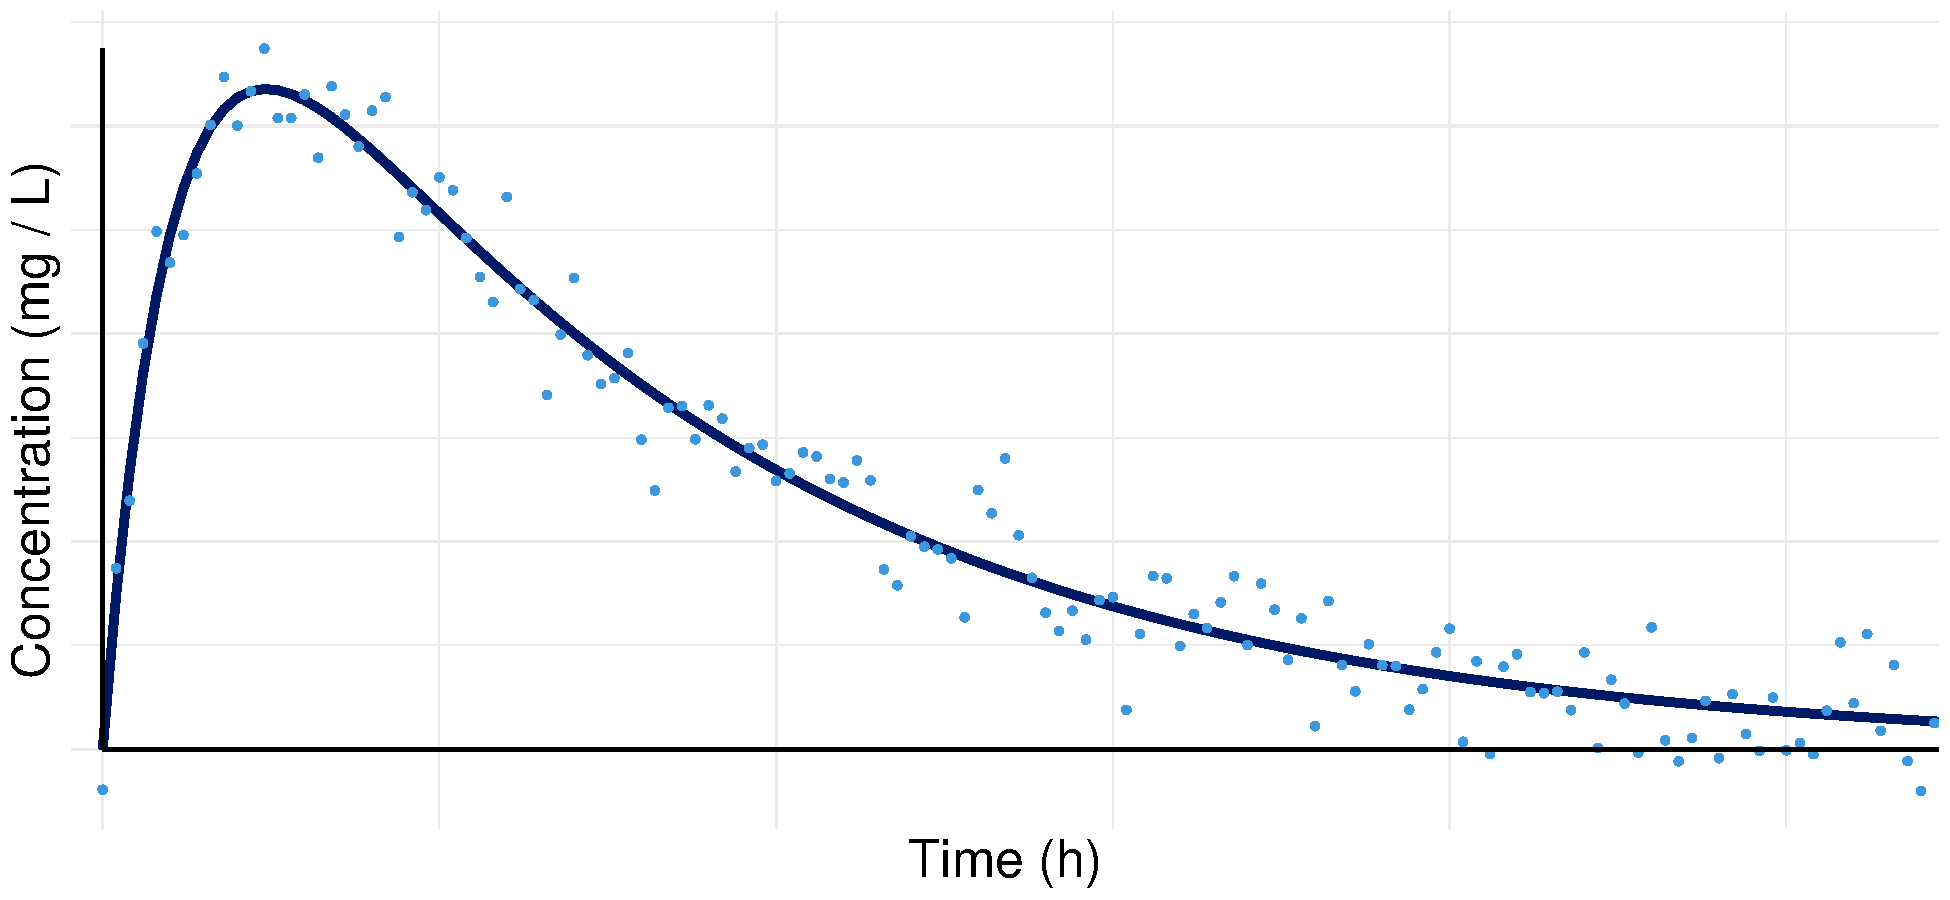
\includegraphics[width=\linewidth]{fig/img/Residual Variance Model/Concentration W. Oral Add.pdf}
%         \caption{Additive error}
%         \label{fig: Residual variance model add}
%     \end{minipage}%
%     \hfill
%     \begin{minipage}{0.45\textwidth}
%         \centering
%         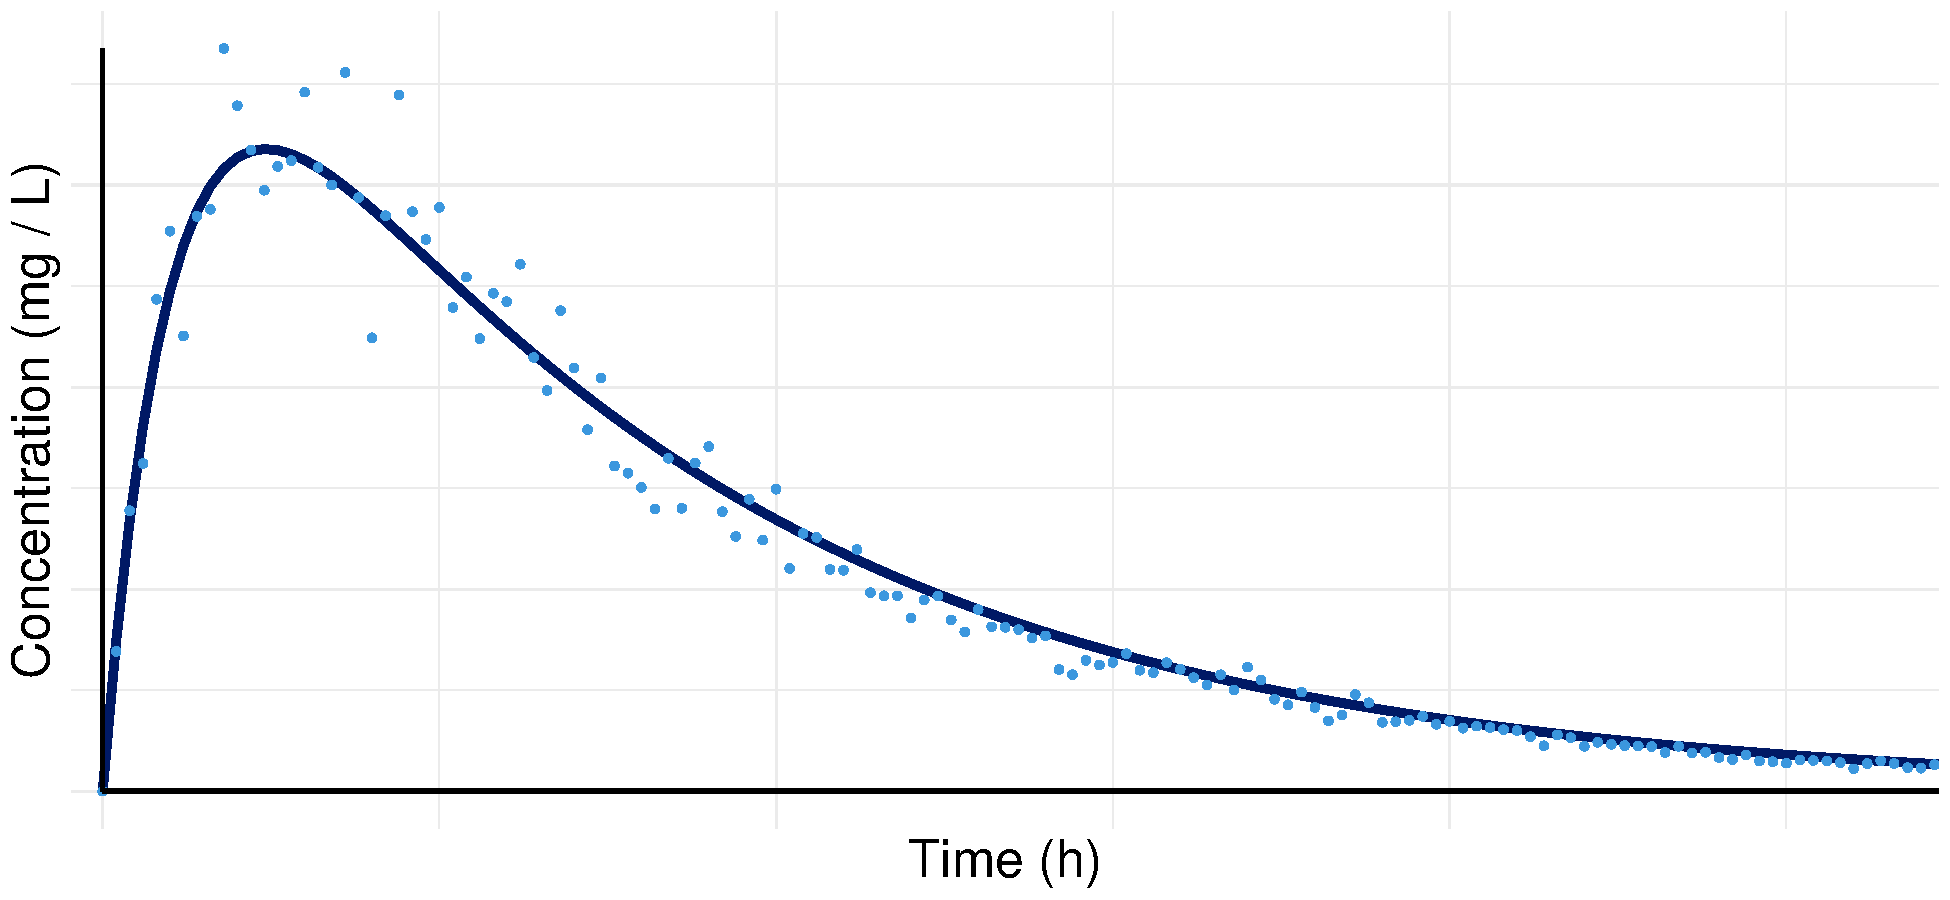
\includegraphics[width=\linewidth]{fig/img/Residual Variance Model/Concentration W. Oral Prop.pdf}
%         \caption{Proportional error}
%         \label{fig: Residual variance model prop}
%     \end{minipage}
%     \vfill

%     \begin{minipage}{0.45\textwidth}
%         \centering
%         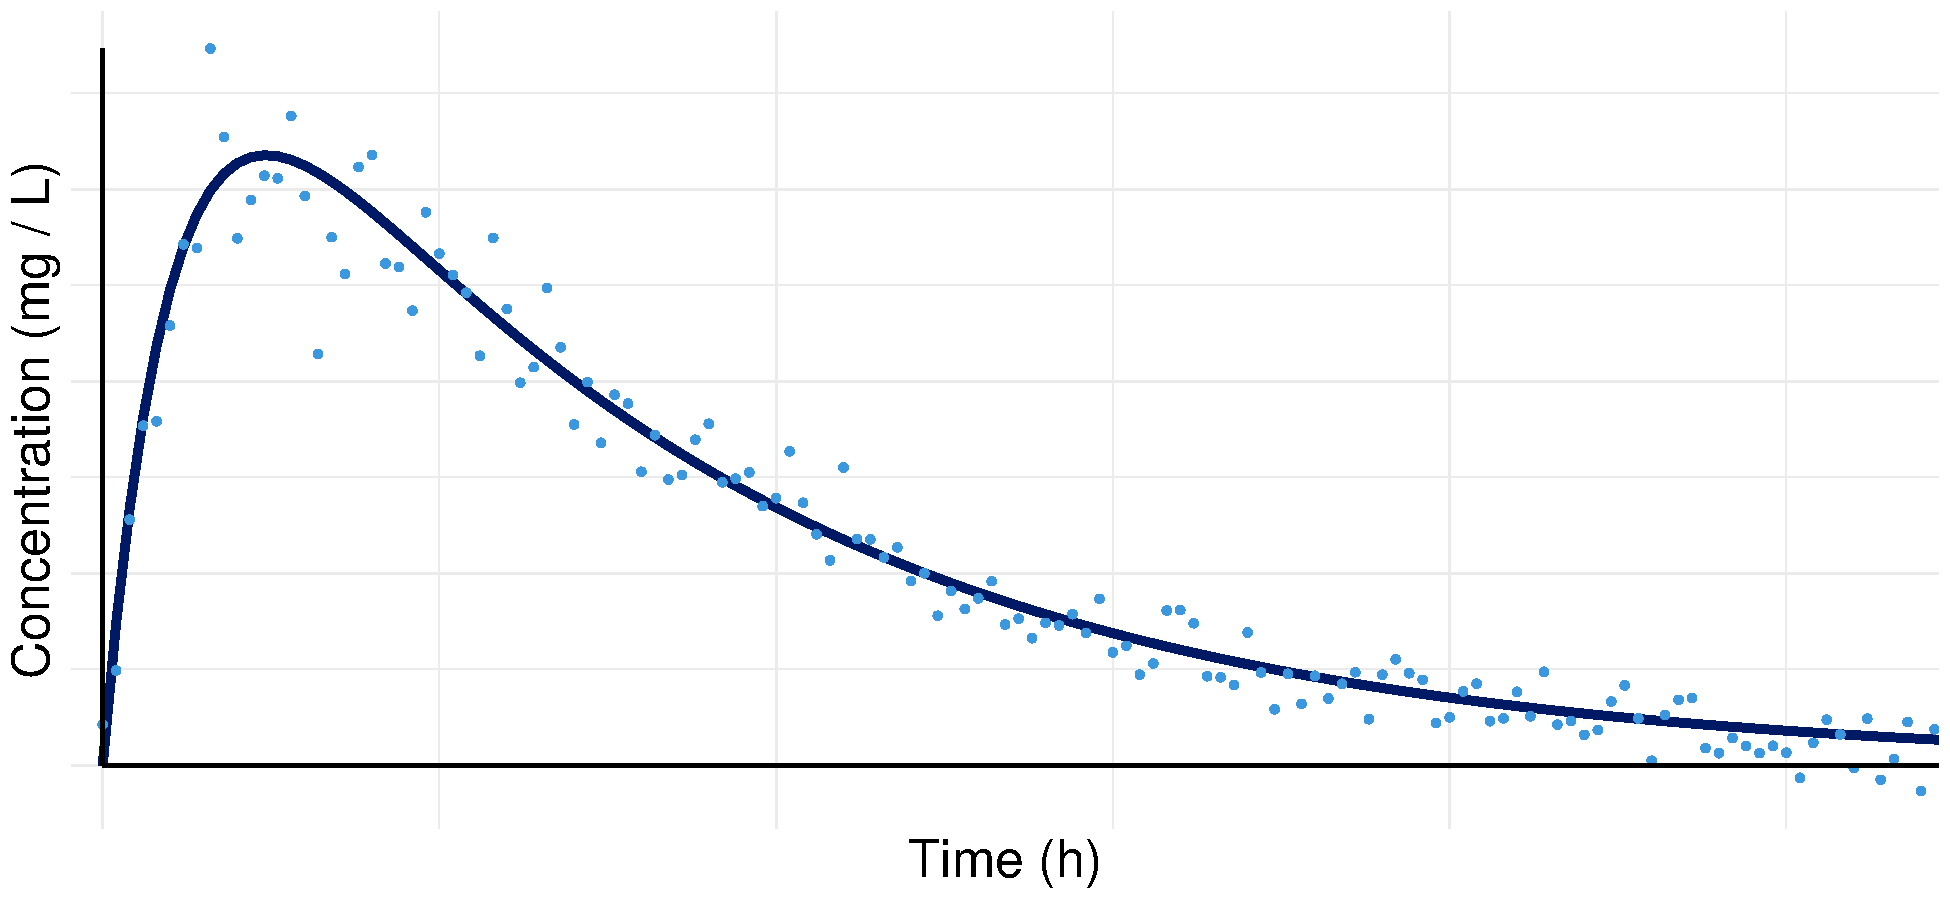
\includegraphics[width=\linewidth]{fig/img/Residual Variance Model/Concentration W. Oral Add Prop.pdf}
%         \caption{Combined additive and proportional error}
%         \label{fig: Residual variance model add prop}
%     \end{minipage}
%     \caption{Simulated concentrations from a single dose one-compartment model with EV administration, each with different residual variance structures.}
%     \label{fig: Residual variance model}
% \end{figure}
% To determine which residual variance model is most suitable, likelihood ratio tests and goodness of fit plots of each model are evaluated. \\













